%%%%%%%%%%%%%%%%%%%%%%%%%%%%% Thesis.tex %%%%%%%%%%%%%%%%%%%%%%%%%%%%%%%
%                                                                      %
%  ---------- Master of Science Dissertation template ----------       %
%                                                                      %
%  Template for the Master Thesis according to the regulations         %
%  published by the Academic Board (Direcção Académica) at IST.        %
%                                                                      %
%  For up-to-date guide, please refer to the official website          %
%  http://academica.tecnico.ulisboa.pt/alunos/dissertacao-de-mestrado/ %
%                                                                      %
%       Andre C. Marta                                                 %
%       Area Cientifica de Mecanica Aplicada e Aeroespacial            %
%       Departamento de Engenharia Mecanica                            %
%       Instituto Superior Tecnico                                     %
%       Av. Rovisco Pais                                               %
%       1049-001 Lisboa                                                %
%       Portugal                                                       %
%       Tel: +351 21 841 9469                                          %
%                        3469 (extension)                              %
%       Email: andre.marta@tecnico.ulisboa.pt                          %
%                                                                      %
%  Created:       Jan 20, 2011                                         %
%  Last Modified: Feb 19, 2018                                         %
%                                                                      %
%%%%%%%%%%%%%%%%%%%%%%%%%%%%%%%%%%%%%%%%%%%%%%%%%%%%%%%%%%%%%%%%%%%%%%%%
%  Revision history                                                    %
%  v1 - 2011/01/24 - original template                                 %
%  v2 - 2012/10/30 - new IST image and glossary support                %
%  v3 - 2013/12/10 - update according to 2012/13 official guide        %
%  v4 - 2014/02/28 - new default for bibliography style                %
%  v5 - 2014/05/07 - update according to 2013/14 official guide        %
%  v6 - 2015/07/02 - cover page format fixed,                          %
%                    contents page numbering fixed,                    %
%                    better language support,                          %
%                    enhanced examples of tables,                      %
%                    new option for appendix page numbering format,    %
%                    custom bibliography style                         %
%  v7 - 2018/02/19 - multiple citations compressed                     %
%%%%%%%%%%%%%%%%%%%%%%%%%%%%%%%%%%%%%%%%%%%%%%%%%%%%%%%%%%%%%%%%%%%%%%%%
%                                                                      %
% To generate the PDF file, type "make" at the terminal prompt.        %
%                                                                      %
% The IST template LaTeX package was created by the author             %
% and it can be downloaded from:                                       %
% https://fenix.ist.utl.pt/homepage/ist31052/                          %
%                                                                      %
% The external packages can be downloaded from                         %
% the Comprehensive TeX Archive Network at http://www.ctan.org/        %
%                                                                      %
% List of LaTex symbols:                                               %
% http://www.ctan.org/tex-archive/info/symbols/comprehensive/          %
%                                                                      %
% Help with LaTex can be found at                                      %
% http://www.giss.nasa.gov/tools/latex/ltx-2.html                      %
% http://en.wikibooks.org/wiki/LaTeX                                   %
%%%%%%%%%%%%%%%%%%%%%%%%%%%%%%%%%%%%%%%%%%%%%%%%%%%%%%%%%%%%%%%%%%%%%%%%

%%%%%%%%%%%%%%%%%%%%%%%%%%%%%%%%%%%%%%%%%%%%%%%%%%%%%%%%%%%%%%%%%%%%%%%%
%     Preamble                                                         %
%%%%%%%%%%%%%%%%%%%%%%%%%%%%%%%%%%%%%%%%%%%%%%%%%%%%%%%%%%%%%%%%%%%%%%%%

% ----------------------------------------------------------------------
%  Set the document class
% ----------------------------------------------------------------------
\documentclass[10pt,a4paper,twoside]{report}

% ----------------------------------------------------------------------
% Define external packages, language, margins, fonts and new commands
% ----------------------------------------------------------------------
%%%%%%%%%%%%%%%%%%%%%%%%%%%%%%%%%%%%%%%%%%%%%%%%%%%%%%%%%%%%%%%%%%%%%%%%
%                                                                      %
%     File: Thesis_Preamble.tex                                        %
%     Tex Master: Thesis.tex                                           %
%                                                                      %
%     Author: Andre C. Marta                                           %
%     Last modified : 9 Apr 2015                                       %
%                                                                      %
%%%%%%%%%%%%%%%%%%%%%%%%%%%%%%%%%%%%%%%%%%%%%%%%%%%%%%%%%%%%%%%%%%%%%%%%

% ----------------------------------------------------------------------
% Define document language.
% ----------------------------------------------------------------------

% 'inputenc' package
%
% Accept different input encodings.
% http://www.ctan.org/tex-archive/macros/latex/base/
%
% > allows typing non-english text in LaTeX sources.
%
% ******************************* SELECT *******************************
%\usepackage[latin1]{inputenc} % <<<<< Windows
\usepackage[utf8]{inputenc}   % <<<<< Linux
% ******************************* SELECT *******************************


% 'babel' package
%
% Multilingual support for Plain TeX or LaTeX.
% http://www.ctan.org/tex-archive/macros/latex/required/babel/
%
% > sets the variable names according to the language selected
%
% ******************************* SELECT *******************************
%\usepackage[portuguese]{babel} % <<<<< Portuguese
\usepackage[english]{babel} % <<<<< English
% ******************************* SELECT *******************************


% List of LaTeX variable names: \abstractname, \appendixname, \bibname,
%   \chaptername, \contentsname, \listfigurename, \listtablename, ...)
% http://www.tex.ac.uk/cgi-bin/texfaq2html?label=fixnam
%
% Changing the words babel uses (uncomment and redefine as necessary...)
%
\newcommand{\acknowledgments}{@undefined} % new LaTeX variable name
%
% > English
%
\addto\captionsenglish{\renewcommand{\acknowledgments}{Acknowledgments}}
%\addto\captionsenglish{\renewcommand{\contentsname}{Contents}}
%\addto\captionsenglish{\renewcommand{\listtablename}{List of Tables}}
%\addto\captionsenglish{\renewcommand{\listfigurename}{List of Figures}}
%\addto\captionsenglish{\renewcommand{\nomname}{Nomenclature}}
%\addto\captionsenglish{\renewcommand{\glossaryname}{Glossary}}
\addto\captionsenglish{\renewcommand{\acronymname}{List of Acronyms}}
%\addto\captionsenglish{\renewcommand{\bibname}{References}} % Bibliography
%\addto\captionsenglish{\renewcommand{\appendixname}{Appendix}}

% > Portuguese
%
\addto\captionsportuguese{\renewcommand{\acknowledgments}{Agradecimentos}}
%\addto\captionsportuguese{\renewcommand{\contentsname}{Conte\'{u}do}}
%\addto\captionsportuguese{\renewcommand{\listtablename}{Lista de Figuras}}
%\addto\captionsportuguese{\renewcommand{\listfigurename}{Lista de Tabelas}}
\addto\captionsportuguese{\renewcommand{\nomname}{Lista de S\'{i}mbolos}} % Nomenclatura
%\addto\captionsportuguese{\renewcommand{\glossary}{Gloss\'{a}rio}}
%\addto\captionsportuguese{\renewcommand{\acronymname}{Lista de Abrevia\c{c}\~{o}es}}
%\addto\captionsportuguese{\renewcommand{\bibname}{Refer\^{e}ncias}} % Bibliografia
%\addto\captionsportuguese{\renewcommand{\appendixname}{Anexo}} % Apendice


% ----------------------------------------------------------------------
% Define cover fields in both english and portuguese.
% ----------------------------------------------------------------------
%
\newcommand{\coverThesis}{@undefined} % new LaTeX variable name
\newcommand{\coverSupervisors}{@undefined} % new LaTeX variable name
\newcommand{\coverExaminationCommittee}{@undefined} % new LaTeX variable name
\newcommand{\coverChairperson}{@undefined} % new LaTeX variable name
\newcommand{\coverSupervisor}{@undefined} % new LaTeX variable name
\newcommand{\coverMemberCommittee}{@undefined} % new LaTeX variable name
% > English
\addto\captionsenglish{\renewcommand{\coverThesis}{Thesis to obtain the Master of Science Degree in}}
\addto\captionsenglish{\renewcommand{\coverSupervisors}{Supervisor(s)}}
\addto\captionsenglish{\renewcommand{\coverExaminationCommittee}{Examination Committee}}
\addto\captionsenglish{\renewcommand{\coverChairperson}{Chairperson}}
\addto\captionsenglish{\renewcommand{\coverSupervisor}{Supervisor}}
\addto\captionsenglish{\renewcommand{\coverMemberCommittee}{Member of the Committee}}
% > Portuguese
\addto\captionsportuguese{\renewcommand{\coverThesis}{Disserta\c{c}\~{a}o para obten\c{c}\~{a}o do Grau de Mestre em}}
\addto\captionsportuguese{\renewcommand{\coverSupervisors}{Orientador(es)}}
\addto\captionsportuguese{\renewcommand{\coverExaminationCommittee}{J\'{u}ri}}
\addto\captionsportuguese{\renewcommand{\coverChairperson}{Presidente}}
\addto\captionsportuguese{\renewcommand{\coverSupervisor}{Orientador}}
\addto\captionsportuguese{\renewcommand{\coverMemberCommittee}{Vogal}}


% ----------------------------------------------------------------------
% Define default and cover page fonts.
% ----------------------------------------------------------------------

% Use Arial font as default
%
\renewcommand{\rmdefault}{phv}
\renewcommand{\sfdefault}{phv}

% Define cover page fonts
%
%         encoding     family       series      shape
%  \usefont{T1}     {phv}=helvetica  {b}=bold    {n}=normal
%                   {ptm}=times      {m}=normal  {sl}=slanted
%                                                {it}=italic
% see more examples at
% http://julien.coron.free.fr/languages/latex/fonts/
%
\def\FontLn{% 16 pt normal
  \usefont{T1}{phv}{m}{n}\fontsize{16pt}{16pt}\selectfont}
\def\FontLb{% 16 pt bold
  \usefont{T1}{phv}{b}{n}\fontsize{16pt}{16pt}\selectfont}
\def\FontMn{% 14 pt normal
  \usefont{T1}{phv}{m}{n}\fontsize{14pt}{14pt}\selectfont}
\def\FontMb{% 14 pt bold
  \usefont{T1}{phv}{b}{n}\fontsize{14pt}{14pt}\selectfont}
\def\FontSn{% 12 pt normal
  \usefont{T1}{phv}{m}{n}\fontsize{12pt}{12pt}\selectfont}


% ----------------------------------------------------------------------
% Define page margins and line spacing.
% ----------------------------------------------------------------------

% 'geometry' package
%
% Flexible and complete interface to document dimensions.
% http://www.ctan.org/tex-archive/macros/latex/contrib/geometry/
%
% > set the page margins (2.5cm minimum in every side, as per IST rules)
%
\usepackage{geometry}	
\geometry{verbose,tmargin=2.5cm,bmargin=2.5cm,lmargin=2.5cm,rmargin=2.5cm}

% 'setspace' package
%
% Set space between lines.
% http://www.ctan.org/tex-archive/macros/latex/contrib/setspace/
%
% > allow setting line spacing (line spacing of 1.5, as per IST rules)
%
\usepackage{setspace}
\renewcommand{\baselinestretch}{1.5}


% ----------------------------------------------------------------------
% Include external packages.
% Note that not all of these packages may be available on all system
% installations. If necessary, include the .sty files locally in
% the <jobname>.tex file directory.
% ----------------------------------------------------------------------

% 'graphicx' package
%
% Enhanced support for graphics.
% http://www.ctan.org/tex-archive/macros/latex/required/graphics/
%
% > extends arguments of the \includegraphics command
%
\usepackage{graphicx}


% 'color' package
%
% Colour control for LaTeX documents.
% http://www.ctan.org/tex-archive/macros/latex/required/graphics/
%
% > defines color macros: \color{<color name>}
%
%\usepackage{color}


% 'amsmath' package
%
% Mathematical enhancements for LaTeX.
% http://www.ctan.org/tex-archive/macros/latex/required/amslatex/
%
% > American Mathematical Society plain Tex macros
%
\usepackage{amsmath}  % AMS mathematical facilities for LaTeX.
\usepackage{amsthm}   % Typesetting theorems (AMS style).
\usepackage{amsfonts} % 


% 'wrapfig' package
%
% Produces figures which text can flow around.
% http://www.ctan.org/tex-archive/macros/latex/contrib/wrapfig/
%
% > wrap figures/tables in text (i.e., Di Vinci style)
%
% \usepackage{wrapfig}


% 'subfigure' package
%
% Deprecated: Figures divided into subfigures.
% http://www.ctan.org/tex-archive/obsolete/macros/latex/contrib/subfigure/
%
% > subcaptions for subfigures
%
\usepackage{subfigure}


% 'subfigmat' package
%
% Automates layout when using the subfigure package.
% http://www.ctan.org/tex-archive/macros/latex/contrib/subfigmat/
%
% > matrices of similar subfigures
%
\usepackage{subfigmat}


% 'url' package
%
% Verbatim with URL-sensitive line breaks.
% http://www.ctan.org/tex-archive/macros/latex/contrib/url/
%
% > URLs in BibTex
%
% \usepackage{url}


% 'varioref' package
%
% Intelligent page references.
% http://www.ctan.org/tex-archive/macros/latex/required/tools/
%
% > smart page, figure, table and equation referencing
%
%\usepackage{varioref}


% 'dcolumn' package
%
% Align on the decimal point of numbers in tabular columns.
% http://www.ctan.org/tex-archive/macros/latex/required/tools/
%
% > decimal-aligned tabular math columns
%
\usepackage{dcolumn}
\newcolumntype{d}{D{.}{.}{-1}} % column aligned by the point separator '.'
\newcolumntype{e}{D{E}{E}{-1}} % column aligned by the exponent 'E'


% 'verbatim' package
%
% Reimplementation of and extensions to LaTeX verbatim.
% http://www.ctan.org/tex-archive/macros/latex/required/tools/
%
% > provides the verbatim environment (\begin{verbatim},\end{verbatim})
%   and a comment environment (\begin{comment},  \end{comment})
%
% \usepackage{verbatim}


% 'moreverb' package
%
% Extended verbatim.
% http://www.ctan.org/tex-archive/macros/latex/contrib/moreverb/
%
% > supports tab expansion and line numbering
%
% \usepackage{moreverb}



% 'nomencl' package
%
% Produce lists of symbols as in nomenclature.
% http://www.ctan.org/tex-archive/macros/latex/contrib/nomencl/
%
% The nomencl package makes use of the MakeIndex program
% in order to produce the nomenclature list.
%
% Nomenclature
% 1) On running the file through LATEX, the command \makenomenclature
%    in the preamble instructs it to create/open the nomenclature file
%    <jobname>.nlo corresponding to the LATEX file <jobname>.tex and
%    writes the information from the \nomenclature commands to this file.
% 2) The next step is to invoke MakeIndex in order to produce the
%    <jobname>.nls file. This can be achieved by making use of the
%    command: makeindex <jobname>.nlo -s nomencl.ist -o <jobname>.nls
% 3) The last step is to invoke LATEX on the <jobname>.tex file once
%    more. There, the \printnomenclature in the document will input the
%    <jobname>.nls file and process it according to the given options.
%
% http://www-h.eng.cam.ac.uk/help/tpl/textprocessing/nomencl.pdf
%
% Nomenclature (produces *.nlo *.nls files)
\usepackage{nomencl}
\makenomenclature
%
% Group variables according to their symbol type
%
\RequirePackage{ifthen} 
\ifthenelse{\equal{\languagename}{english}}%
    { % English
    \renewcommand{\nomgroup}[1]{%
      \ifthenelse{\equal{#1}{R}}{%
        \item[\textbf{Roman symbols}]}{%
        \ifthenelse{\equal{#1}{G}}{%
          \item[\textbf{Greek symbols}]}{%
          \ifthenelse{\equal{#1}{S}}{%
            \item[\textbf{Subscripts}]}{%
            \ifthenelse{\equal{#1}{T}}{%
              \item[\textbf{Superscripts}]}{}}}}}%
    }{% Portuguese
    \renewcommand{\nomgroup}[1]{%
      \ifthenelse{\equal{#1}{R}}{%
        \item[\textbf{Simbolos romanos}]}{%
        \ifthenelse{\equal{#1}{G}}{%
          \item[\textbf{Simbolos gregos}]}{%
          \ifthenelse{\equal{#1}{S}}{%
            \item[\textbf{Subscritos}]}{%
            \ifthenelse{\equal{#1}{T}}{%
              \item[\textbf{Sobrescritos}]}{}}}}}%
    }%


% 'glossary' package
%
% Create a glossary.
% http://www.ctan.org/tex-archive/macros/latex/contrib/glossary/
%
% Glossary (produces *.glo *.ist files)
\usepackage[number=none]{glossary}
% (remove blank line between groups)
\setglossary{gloskip={}}
% (redefine glossary style file)
%\renewcommand{\istfilename}{myGlossaryStyle.ist}
\makeglossary


% 'rotating' package
%
% Rotation tools, including rotated full-page floats.
% http://www.ctan.org/tex-archive/macros/latex/contrib/rotating/
%
% > show wide figures and tables in landscape format:
%   use \begin{sidewaystable} and \begin{sidewaysfigure}
%   instead of 'table' and 'figure', respectively.
%
\usepackage{rotating}


% 'hyperref' package
%
% Extensive support for hypertext in LaTeX.
% http://www.ctan.org/tex-archive/macros/latex/contrib/hyperref/
%
% > Extends the functionality of all the LATEX cross-referencing
%   commands (including the table of contents, bibliographies etc) to
%   produce \special commands which a driver can turn into hypertext
%   links; Also provides new commands to allow the user to write adhoc
%   hypertext links, including those to external documents and URLs.
%
\usepackage[pdftex]{hyperref} % enhance documents that are to be
                              % output as HTML and PDF
\hypersetup{colorlinks,       % color text of links and anchors,
                              % eliminates borders around links
%            linkcolor=red,    % color for normal internal links
            linkcolor=black,  % color for normal internal links
            anchorcolor=black,% color for anchor text
%            citecolor=green,  % color for bibliographical citations
            citecolor=black,  % color for bibliographical citations
%            filecolor=magenta,% color for URLs which open local files
            filecolor=black,  % color for URLs which open local files
%            menucolor=red,    % color for Acrobat menu items
            menucolor=black,  % color for Acrobat menu items
%            pagecolor=red,    % color for links to other pages
            pagecolor=black,  % color for links to other pages
%            urlcolor=cyan,    % color for linked URLs
            urlcolor=black,   % color for linked URLs
	          bookmarks=true,         % create PDF bookmarks
	          bookmarksopen=false,    % don't expand bookmarks
	          bookmarksnumbered=true, % number bookmarks
	          pdftitle={Thesis},
            pdfauthor={Andre C. Marta},
            pdfsubject={Thesis Title},
            pdfkeywords={Thesis Keywords},
            pdfstartview=FitV,
            pdfdisplaydoctitle=true}


% 'hypcap' package
%
% Adjusting the anchors of captions.
% http://www.ctan.org/tex-archive/macros/latex/contrib/oberdiek/
%
% > fixes the problem with hyperref, that links to floats points
%   below the caption and not at the beginning of the float.
%
\usepackage[figure,table]{hypcap}


% 'natbib' package
%
% Flexible bibliography support.
% http://www.ctan.org/tex-archive/macros/latex/contrib/natbib/
%
% > produce author-year style citations
%
% \citet  and \citep  for textual and parenthetical citations, respectively
% \citet* and \citep* that print the full author list, and not just the abbreviated one
% \citealt is the same as \citet but without parentheses. Similarly, \citealp is \citep without parentheses
% \citeauthor
% \citeyear
% \citeyearpar
%
%% natbib options can be provided when package is loaded \usepackage[options]{natbib}
%%
%% Following options are valid:
%%
%%   round  -  round parentheses are used (default)
%%   square -  square brackets are used   [option]
%%   curly  -  curly braces are used      {option}
%%   angle  -  angle brackets are used    <option>
%%   semicolon  -  multiple citations separated by semi-colon (default)
%%   colon  - same as semicolon, an earlier confusion
%%   comma  -  separated by comma
%%   authoryear - for author–year citations (default)
%%   numbers-  selects numerical citations
%%   super  -  numerical citations as superscripts, as in Nature
%%   sort   -  sorts multiple citations according to order in ref. list
%%   sort&compress   -  like sort, but also compresses numerical citations
%%   compress - compresses without sorting
%%
% ******************************* SELECT *******************************
%\usepackage{natbib}          % <<<<< References in alphabetical list Correia, Silva, ...
\usepackage[numbers,sort&compress]{natbib} % <<<<< References in numbered list [1],[2],...
% ******************************* SELECT *******************************


% 'notoccite' package
%
% Prevent trouble from citations in table of contents, etc.
% http://ctan.org/pkg/notoccite
%
% > If you have \cite com­mands in \sec­tion-like com­mands, or in \cap­tion,
%   the ci­ta­tion will also ap­pear in the ta­ble of con­tents, or list of what­ever.
%   If you are also us­ing an un­srt-like bib­li­og­ra­phy style, these ci­ta­tions will
%   come at the very start of the bib­li­og­ra­phy, which is con­fus­ing. This pack­age
%   sup­presses the ef­fect.
%
\usepackage{notoccite}


% 'multirow' package
%
% Create tabular cells spanning multiple rows
% http://www.ctan.org/pkg/multirow
%
\usepackage{multirow}


% 'booktabs' package
%
% Publication quality tables in LaTeX
% http://www.ctan.org/pkg/booktabs
%
% > en­hance the qual­ity of ta­bles in LaTeX, pro­vid­ing ex­tra com­mands.
%
% \renewcommand{\arraystretch}{<ratio>} % space between rows
%
\usepackage{booktabs}
%\newcommand{\ra}[1]{\renewcommand{\arraystretch}{#1}}


% 'pdfpages' package
%
% Include PDF documents in LaTeX
% http://www.ctan.org/pkg/pdfpages
%
% > in­clu­sion of ex­ter­nal multi-page PDF doc­u­ments in LaTeX doc­u­ments.
%   Pages may be freely se­lected and sim­i­lar to psnup it is pos­si­ble to put
%   sev­eral log­i­cal pages onto each sheet of pa­per.
%
% \includepdf{filename.pdf}
% \includepdf[pages={4-9},nup=2x3,landscape=true]{filename.pdf}
%
\usepackage{pdfpages}


% ----------------------------------------------------------------------
% Define new commands to assure consistent treatment throughout document
% ----------------------------------------------------------------------

\newcommand{\ud}{\mathrm{d}}                % total derivative
\newcommand{\degree}{\ensuremath{^\circ\,}} % degrees

% Abbreviations

\newcommand{\mcol}{\multicolumn}            % table format

\newcommand{\eqnref}[1]{(\ref{#1})}
\newcommand{\class}[1]{\texttt{#1}}
\newcommand{\package}[1]{\texttt{#1}}
\newcommand{\file}[1]{\texttt{#1}}
\newcommand{\BibTeX}{\textsc{Bib}\TeX}

% Typefaces ( example: {\bf Bold text here} )
%
% > pre-defined
%   \bf % bold face
%   \it % italic
%   \tt % typewriter
%
% > newly defined
\newcommand{\tr}[1]{{\ensuremath{\textrm{#1}}}}   % text roman
\newcommand{\tb}[1]{{\ensuremath{\textbf{#1}}}}   % text bold face
\newcommand{\ti}[1]{{\ensuremath{\textit{#1}}}}   % text italic
\newcommand{\mc}[1]{{\ensuremath{\mathcal{#1}}}}  % math calygraphy
\newcommand{\mco}[1]{{\ensuremath{\mathcalold{#1}}}}% math old calygraphy
\newcommand{\mr}[1]{{\ensuremath{\mathrm{#1}}}}   % math roman
\newcommand{\mb}[1]{{\ensuremath{\mathbf{#1}}}}   % math bold face
\newcommand{\bs}[1]{\ensuremath{\boldsymbol{#1}}} % math symbol
\def\bm#1{\mathchoice                             % math bold
  {\mbox{\boldmath$\displaystyle#1$}}%
  {\mbox{\boldmath$#1$}}%
  {\mbox{\boldmath$\scriptstyle#1$}}%
  {\mbox{\boldmath$\scriptscriptstyle#1$}}}
\newcommand{\boldcal}[1]{{\ensuremath{\boldsymbol{\mathcal{#1}}}}}% math bold calygraphy



\usepackage[acronym,nomain,nonumberlist, section=chapter]{glossaries}
\makeglossaries




\newacronym{gpu}{GPU}{Graphical Processing Unit}
\newacronym{gpgpu}{GPGPU}{General Purpose Graphical Processing Unit}
\newacronym{cpu}{CPU}{Central Processing Unit}
\newacronym{hsa}{HSA}{Heterogeneous System Architecture}
\newacronym{api}{API}{Application Protocol Interface}
\newacronym{simt}{SIMT}{Single Instruction Multiple Threads}
\newacronym{roc}{ROC}{Radeon Open Computing platform}
\newacronym{risc}{RISC}{Reduced Instruction Set Computer}


\newacronym{cmos}{CMOS}{Complementary metal-oxide-semiconductor}
\newacronym{pvt}{PVT}{Process, Voltage and Temperature}
\newacronym{bti}{BTI}{Bias temperature instability}
\newacronym{hci}{HCI}{Hot Carrier Injection}
\newacronym{dvfs}{DVFS}{Dynamic Voltage and Frequency Scaling}
\newacronym{afvs}{AFVS}{Adaptive Frequency and Voltage Scaling}
\newacronym{sm}{SM}{Streaming Multiprocessor}
\newacronym{cu}{CU}{Computing Unit}
\newacronym{ncu}{NCU}{Next Compute Unit}
\newacronym{dram}{DRAM}{Dynamic Random-Access Memory}
\newacronym{apsa}{ApSA}{Application-aware Scalable Architecture}
\newacronym{edp}{EDP}{Energy Delay Product}
\newacronym{alu}{ALU}{Arithmetic and Logic Unit}
\newacronym{mac}{MAC}{Multiply and Accumulate}
\newacronym{sfu}{SFU}{Special Function Unit}


\newacronym{dl}{DL}{Deep Learning}
\newacronym{dnn}{DNN}{Deep Neural Network}
\newacronym{cnn}{CNN}{Convolutional Neural Network}
\newacronym{rnn}{RNN}{Recurrent Neural Network}
\newacronym{upt}{UPT}{Unsupervised Pre-trained Network}
\newacronym{gan}{GAN}{Generative Adversarial Network}
\newacronym{sgd}{SGD}{ Stochastic Gradient Descent}
 % file "Thesis_Acronyms.tex"
\glsaddall

\usepackage{indentfirst}

\usepackage{amsmath,amssymb,amsfonts}
\usepackage{algorithm, algorithmic}
\usepackage{listings}
\usepackage{rotating}
\usepackage{tikz}
\patchcmd{\subfigmatrix}{\hfill}{\hspace{0.8cm}}{}{} % file "Thesis_Preamble.tex"

%%%%%%%%%%%%%%%%%%%%%%%%%%%%%%%%%%%%%%%%%%%%%%%%%%%%%%%%%%%%%%%%%%%%%%%%
%     Begin Document                                                   %
%%%%%%%%%%%%%%%%%%%%%%%%%%%%%%%%%%%%%%%%%%%%%%%%%%%%%%%%%%%%%%%%%%%%%%%%
\begin{document}

% Set plain page style (no headers, footer with centered page number)
\pagestyle{plain}

% Set roman numbering (i,ii,...) before the start of chapters
\pagenumbering{roman}

% ----------------------------------------------------------------------
%  Cover page
% ----------------------------------------------------------------------
%%%%%%%%%%%%%%%%%%%%%%%%%%%%%%%%%%%%%%%%%%%%%%%%%%%%%%%%%%%%%%%%%%%%%%%%
%                                                                      %
%     File: Thesis_FrontCover.tex                                      %
%     Tex Master: Thesis.tex                                           %
%                                                                      %
%     Author: Andre C. Marta                                           %
%     Last modified :  2 Jul 2015                                      %
%                                                                      %
%%%%%%%%%%%%%%%%%%%%%%%%%%%%%%%%%%%%%%%%%%%%%%%%%%%%%%%%%%%%%%%%%%%%%%%%

\thispagestyle {empty}

% IST Logo - Signature A
% parameters: bb=llx lly urx ury (bounding box), width=h_length, height=v_length, angle=angle, scale=factor, clip=true/false, draft=true/false. 

\includegraphics[bb=9.5cm 11cm 0cm 0cm,scale=0.29]{IST_A_CMYK_POS}

\begin{center}
%
% Figure (Image or plot)
\vspace{2.5cm}
% height = 50 mm
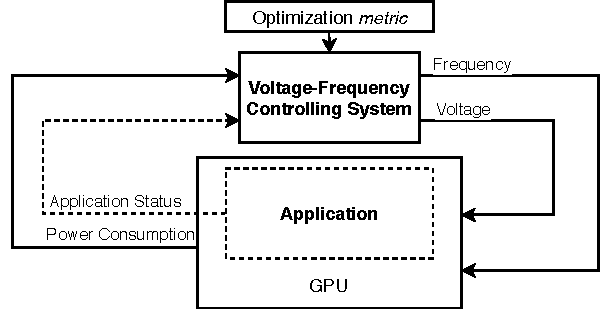
\includegraphics[height=40mm]{Figures/Cover/front_cover.pdf}

% Title, author and degree
\vspace{1.0cm}
{\FontLb Exploiting non-conventional DVFS on GPUs: \\application to Deep Learning} \\ 
%\vspace{0.2cm}
%{\FontMn Subtitle (optional)} \\
%\vspace{1.9cm}
\vspace{2.6cm}
{\FontMb Francisco Soares Mendes} \\ 
\vspace{2.0cm}
{\FontSn \coverThesis} \\
\vspace{0.3cm}
{\FontLb Electrical and Computer Engineering} \\ 
\vspace{1.0cm}
{\FontSn %
\begin{tabular}{ll}
 \coverSupervisors: & Doutor Nuno Filipe Valentim Roma \\
                    & Doutor Pedro Filipe Zeferino Tomás
\end{tabular} } \\
\vspace{1.0cm}
{\FontMb \coverExaminationCommittee} \\
\vspace{0.3cm}
{\FontSn %
\begin{tabular}{c}
\coverChairperson:     Doutora Teresa Maria Sá Ferreira Vazão Vasques         \\
\coverSupervisor:      Doutor Nuno Filipe Valentim Roma \\ 
\coverMemberCommittee: Doutor Luís Miguel Teixeira D'Avila Pinto da Silveira
\end{tabular} } \\
\vspace{1.5cm}
{\FontMb October 2020} \\ % <<<<< EDIT DATE (corresponds to date of oral examination)
%
\end{center}

 % file "Thesis_FrontCover.tex"
\cleardoublepage

% ----------------------------------------------------------------------
% Dedication page (optional)
% ----------------------------------------------------------------------
% %%%%%%%%%%%%%%%%%%%%%%%%%%%%%%%%%%%%%%%%%%%%%%%%%%%%%%%%%%%%%%%%%%%%%%%%
%                                                                      %
%     File: Thesis_Dedication.tex                                      %
%     Tex Master: Thesis.tex                                           %
%                                                                      %
%     Author: Andre C. Marta                                           %
%     Last modified :  2 Jul 2015                                      %
%                                                                      %
%%%%%%%%%%%%%%%%%%%%%%%%%%%%%%%%%%%%%%%%%%%%%%%%%%%%%%%%%%%%%%%%%%%%%%%%

\null\vskip5cm%
\begin{flushright}
     Dedicated to someone special...
\end{flushright}
\vfill\newpage

 % file "Thesis_Dedication.tex"
% \cleardoublepage

% ----------------------------------------------------------------------
%  Acknowledgments (optional)
% ----------------------------------------------------------------------
%%%%%%%%%%%%%%%%%%%%%%%%%%%%%%%%%%%%%%%%%%%%%%%%%%%%%%%%%%%%%%%%%%%%%%%%
%                                                                      %
%     File: Thesis_Acknowledgments.tex                                 %
%     Tex Master: Thesis.tex                                           %
%                                                                      %
%     Author: Andre C. Marta                                           %
%     Last modified :  2 Jul 2015                                      %
%                                                                      %
%%%%%%%%%%%%%%%%%%%%%%%%%%%%%%%%%%%%%%%%%%%%%%%%%%%%%%%%%%%%%%%%%%%%%%%%

\section*{\acknowledgments}

% Add entry in the table of contents as section
\addcontentsline{toc}{section}{\acknowledgments}

A few words about the university, financial support, research advisor, dissertation readers, faculty or other professors, lab mates, other friends and family...

 % file "Thesis_Acknowledgements.tex"
\cleardoublepage

% ----------------------------------------------------------------------
%  Abstract (both in English and Portuguese)
% ----------------------------------------------------------------------
%%%%%%%%%%%%%%%%%%%%%%%%%%%%%%%%%%%%%%%%%%%%%%%%%%%%%%%%%%%%%%%%%%%%%%%%
%                                                                      %
%     File: Thesis_Resumo.tex                                          %
%     Tex Master: Thesis.tex                                           %
%                                                                      %
%     Author: Andre C. Marta                                           %
%     Last modified :  2 Jul 2015                                      %
%                                                                      %
%%%%%%%%%%%%%%%%%%%%%%%%%%%%%%%%%%%%%%%%%%%%%%%%%%%%%%%%%%%%%%%%%%%%%%%%

\section*{Resumo}

% Add entry in the table of contents as section
\addcontentsline{toc}{section}{Resumo}

Atualmente, as unidades de processamento gráfico (do inglês GPUs) são os principais dispositivos computacionais usados para acelerar aplicações de cariz paralelo. Contudo, esse imenso desempenho acarreta um alto consumo energético. Diversas soluções podem ser seguidas para aumentar a eficiência energética desses dispositivos. Porém, o escalonamento de tensão-frequência (T-F) tem sido a solução que obtém melhores resultados, permitindo melhorar as métricas de eficiência energética de forma automática e independente do tipo de aplicações a ser executadas. 

As implementações atuais de escalonamento dinâmico de tensão e frequência (do inglês DVFS) em GPUs são unidimensionais, ajustando a frequência dentro dos pares de tensão-frequência padrão. No entanto, este ajuste é insuficiente, pois não garante o par T-F mais adequado à aplicação a ser executada. Esta dissertação apresenta uma metodologia para caraterizar o impacto do DVFS não convencional em GPUs, capaz de colmatar o carácter unidimensional das implementações actuais. A abordagem proposta cria um espaço de parametrização que determina a faixa de tensão permitida para cada frequência. A mesma foi testada em duas GPUs da AMD com os resultados a mostrarem que ambas são capazes de operar em segurança com até menos 20\% do valor padrão de tensão.
Este espaço de parametrização é então usado pelo mecanismo de otimização T-F desenvolvido para selecionar a configuração de maior eficiência energética. Quando aplicado a aplicações de Aprendizagem Profunda e, especificamente, Redes Neurais Convolucionais, o mecanismo desenvolvido demonstra ser capaz de melhorar a eficiência energética da GPU em até 44\% sem qualquer deterioração medida da precisão do modelo.

\vfill

\textbf{\Large Palavras-chave:} Unidade de Processamento Gráfico, Escalonamento Dinâmico de Tensão e Frequência, Redução da Tensão, Mecanismo de Optimização, Aprendizagem Profunda, Redes Neuronais Profundas.
   % file "Thesis_Resumo.tex"
\cleardoublepage

%%%%%%%%%%%%%%%%%%%%%%%%%%%%%%%%%%%%%%%%%%%%%%%%%%%%%%%%%%%%%%%%%%%%%%%%
%                                                                      %
%     File: Thesis_Abstract.tex                                        %
%     Tex Master: Thesis.tex                                           %
%                                                                      %
%     Author: Andre C. Marta                                           %
%     Last modified :  2 Jul 2015                                      %
%                                                                      %
%%%%%%%%%%%%%%%%%%%%%%%%%%%%%%%%%%%%%%%%%%%%%%%%%%%%%%%%%%%%%%%%%%%%%%%%

\section*{Abstract}

\addcontentsline{toc}{section}{Abstract}

Graphics Processing Units (GPUs) are the primary computational devices used to accelerate highly parallel applications. However, this immense performance comes at the cost of high energy consumption. Several solutions can be followed to increase the energy-efficiency of these devices. Though, Voltage-Frequency (V-F) scaling has been the one that achieves better results by allowing to improve this metric automatically and independently of the workload. 

However, current implementations of Dynamic Voltage and Frequency Scaling (DVFS) on GPUs are still one-dimensional, by simply adjusting frequency while relying on default voltage settings. To overcome this, this dissertation introduces a methodology to fully characterize the impact of non-conventional DVFS in GPUs. The proposed approach creates a Usable Execution Space (UES) that determines the voltage range allowed by each frequency, showing that two out-of-the-shelf AMD GPUs are able to be safely undervolted by more than 20\%. The UES is then used by the devised V-F optimization mechanism to select the most energy-efficiency configuration. When applied to Deep Learning applications and, specifically, Convolutional Neural Networks (CNNs), the mechanism can improve the GPU energy efficiency by up to 44\% without any measured deterioration of the model accuracy.

\vfill

\textbf{\Large Keywords:} Graphics Processing Unit, Dynamic Voltage and Frequency Scaling, Undervoltage, Optimization Mechanism, Deep Learning, Deep Neural Networks.

 % file "Thesis_Abstract.tex"
\cleardoublepage

% ----------------------------------------------------------------------
%  Table of contents, list of tables, list of figures and nomenclature
% ----------------------------------------------------------------------

% Table of contents
%
\tableofcontents
\cleardoublepage 

% List of tables
%
% Add entry in the table of contents as section
\phantomsection
\addcontentsline{toc}{section}{\listtablename}
% Generate list
\listoftables
\cleardoublepage 

% List of figures
%
% Add entry in the table of contents as section
\phantomsection
\addcontentsline{toc}{section}{\listfigurename}
% Generate list
\listoffigures
\cleardoublepage 

% Nomenclature
%
% entries of acronyms list
\phantomsection
\addcontentsline{toc}{section}{List of Acronyms}
\printglossary[type=\acronymtype,title=List of Acronyms]
\cleardoublepage




% Set arabic numbering (1,2,...) after preface
%
\setcounter{page}{1}
\pagenumbering{arabic}

% ----------------------------------------------------------------------
%  Chapters
% ----------------------------------------------------------------------

%%%%%%%%%%%%%%%%%%%%%%%%%%%%%%%%%%%%%%%%%%%%%%%%%%%%%%%%%%%%%%%%%%%%%%%%
%                                                                      %
%     File: Thesis_Introduction.tex                                    %
%     Tex Master: Thesis.tex                                           %
%                                                                      %
%     Author: Francisco Mendes                                           %
%     Last modified :  31 Jul 2020                                      %
%                                                                      %
%%%%%%%%%%%%%%%%%%%%%%%%%%%%%%%%%%%%%%%%%%%%%%%%%%%%%%%%%%%%%%%%%%%%%%%%

\chapter{Introduction}
\label{chapter:introduction}

In the last few years, Deep Neural Networks (\acrshort{dnn}s) have had a significant impact in industry and society by allowing for important breakthroughs in many application domains, such as computer vision, speech recognition, natural language processing, drug discovery, genomics, etc \cite{shrestha_review_2019}.

However, \acrshort{dnn}s are usually characterized by significant computational burdens, particularly when considering the training of very deep and complex networks, dealing with high dimensional data, such as images and videos. For such purpose, researchers (and data scientists, in general) often rely on accelerators, such as Graphical Processing Units (\acrshort{gpu}s), to cope with the associated computational burden and reduce the training time. \acrshort{gpu}s differ from conventional processors by including thousands of computing cores (Compute Units - \acrshort{cu}s) and a large bandwidth memory module. As a result, they are able to execute the same instruction over massive amounts of data. Due to their versatility and compute power, \acrshort{gpu}s are now commonly deployed on most supercomputers, data centers, and other computational infrastructures related to artificial intelligence algorithms' development.



Additionally, several software frameworks, algorithms and techniques have been proposed to manage and optimize the execution of \acrshort{dnn} on \acrshort{gpu} (e.g., the work of Mittal~\cite{mittal_survey_2019}). However, most optimization techniques neglect the training phase's energy impact, usually resulting in considerable costs. 

To overcome this problem, researchers have also explored other solutions that allow mitigating the energy impact of neural network training. One particular and common approach relies on the use of low-precision arithmetic (e.g., demonstrated by Nabavinejad~ \cite{nabavinejad_coordinated_2019}), eventually trading network accuracy with increased processing performance and lower energy consumption.

Researchers have also looked at alternative approaches, such as exploiting Dynamic Voltage and Frequency Scaling (\acrshort{dvfs}) on both the inference and training phases. In fact, by carefully selecting the used voltage-frequency (V-F) levels, significant energy savings can be obtained, although depending on the considered \acrshort{dnn} architecture and computing  device~\cite{tang_impact_2019}. This is achieved through a careful balance between the different GPU components' performance and power consumption (particularly the core and global memory) to minimize stalls in the compute cores. In fact, not only can \acrshort{dvfs} be used to decrease the power consumption, but it can also boost the system performance~\cite{tang_impact_2019}, by increasing the voltage and frequency levels (as long as the GPU total power envelope and thermal limits are not surpassed).

Nevertheless, most state-of-the-art works only consider tightly coupled V-F levels, often predefined by \acrshort{gpu} manufacturers and neglecting the voltage margin that is usually introduced to guarantee fail-safe designs, as well as its variation with the kernel instruction sequence and the corresponding use of specific \acrshort{gpu} components. Supported on this observation, this work tries to increase the energy-efficiency of \acrshort{gpu}s by understanding and characterizing their behavior when subject to non-conventional V-F scaling. 
It also tries to go one step further by creating an optimization mechanism that automatically selects the V-F pair that better suits the running application as well as the specific characteristics of the computing device.


%%%%%%%%%%%%%%%%%%%%%%%%%%%%%%%%%%%%%%%%%%%%%%%%%%%%%%%%%%%%%%%%%%%%%%%%
\section{Objectives}
\label{section:objectives}

To uncover the use of non-conventional V-F scaling, this thesis focuses on the following objectives:

\begin{itemize}
\item Access the viability of using non-conventional V-F pairs on regular \acrshort{gpu}s.
\item Characterize the behaviour of the \acrshort{gpu} architecture to non-conventional V-F pairs.
\item Develop an automatic non-conventional V-F controlling and optimization mechanism that improves the \textit{performance}, \textit{energy consumption} or \textit{energy-efficiency} of \acrshort{gpu}s.
\item Safely apply non-conventional V-F scaling on Deep Learning applications, characterizing the behaviour of training procedure.
\end{itemize}


%%%%%%%%%%%%%%%%%%%%%%%%%%%%%%%%%%%%%%%%%%%%%%%%%%%%%%%%%%%%%%%%%%%%%%%%
\section{Main Contributions}
\label{section:main_contri}


\textcolor{red}{FALAR DO QUE FOI FEITO}

The scientific contributions of this work have been published for communication in the following conference:

\begin{itemize}
    \item F. Mendes, P. Tómas and N. Roma, "Exploiting non-conventional DVFS on GPUs: application to Deep Learning", IEEE 32nd International Symposium on Computer Architecture and High Performance Computing, 2020.
\end{itemize}


%%%%%%%%%%%%%%%%%%%%%%%%%%%%%%%%%%%%%%%%%%%%%%%%%%%%%%%%%%%%%%%%%%%%%%%%
\section{Dissertation Outline}
\label{section:outline}
\textcolor{red}{ACABAR DE DESCREVER CADA CAPITULO}
This dissertation is organized in 4 chapters with the following outline:
\begin{itemize}
    \item Chapter 2 - Background: This chapter presents a summary of the current state-of-the art related with the subject in study.
    \item Chapter 3 - GPU architectural characterization to decoupled V-F:
    \item Chapter 4 - V-F Optimization Mechanism:
    \item Chapter 5 - Application to Deep Learning:
    \item Chapter 6 - Conclusions:
\end{itemize}

 % file "Thesis_Introduction.tex"
\cleardoublepage

%%%%%%%%%%%%%%%%%%%%%%%%%%%%%%%%%%%%%%%%%%%%%%%%%%%%%%%%%%%%%%%%%%%%%%%%
%                                                                      %
%     File: Thesis_Background.tex                                      %
%     Tex Master: Thesis.tex                                           %
%                                                                      %
%     Author: Francisco Mendes                                         %
%     Last modified :  31 Jul 2020                                     %
%                                                                      %
%%%%%%%%%%%%%%%%%%%%%%%%%%%%%%%%%%%%%%%%%%%%%%%%%%%%%%%%%%%%%%%%%%%%%%%%

\chapter{Background}
\label{chapter:background}

This chapter provides an overview of modern \acrshort{gpu} architecture and respective programming models that allow the extensive use of these devices to execute more computationally intensive applications, followed by an analysis of techniques to improve the energy efficiency of the same. 

The following sections present a bottom-up sequence of background and related work that supports this thesis — starting by the physical analysis of the digital circuits and the effects of V-F scaling and temperature on them. It continues by presenting the most common procedure to improve \acrshort{gpu}s energy efficiency (\acrshort{dvfs}) and finishes by exploring the techniques that will allow for further improvements to these device based on a complete decoupling between the applied voltage supply and operating frequency. 

The relevance of the presented work emerges from the reduced number of studies on the effects of decoupled voltage scaling on \acrshort{gpu}s, one of the objectives of this dissertation. The main reason is probably mainly due to lack of support for independently controlling these parameters on NVIDIA \acrshort{gpu}s (until recently, the dominant player on the market \cite{noauthor_jon_2018, mujtaba_amd_2019}) that is now allowed by the novel AMD software stack used on this work.






%%%%%%%%%%%%%%%%%%%%%%%%%%%%%%%%%%%%%%%%%%%%%%%%%%%%%%%%%%%%%%%%%%%%%%%%
\section{General Purpose Computing on GPUs}
\label{section:gpp_gpu}

A \acrshort{gpu} is a highly parallel programmable processor, that favours the execution of the same instruction on multiple data elements, belonging to the category of \textit{Single Instruction Multiple Threads} - \acrshort{simt} processors. When referring to \acrshort{gpu}s, it is still common to be talking about their graphics capabilities. However, more and more programs are taking advantage of their highly parallel architecture to accelerate general purpose applications, leading to the connotation of this device as a \acrshort{gpgpu} - General Purpose Graphical Processing Unit.

The development and deployment of \acrshort{gpgpu} applications are only possible with the creation and adoption of standardized programming models and APIs that allow for hardware abstraction. This section provides a general overview of the \acrshort{gpu} architecture, followed by the presentation of the most common and used software tools available for \acrshort{gpgpu} programming.




\subsection{General Overview of a GPU Architecture}
The architecture of a modern \acrshort{gpu}, depicted in figure~\ref{fig:Vega10arch}, can be roughly divided into computation and memory components. The computation part is usually composed of the vertex shader, the rendering engine, and the \acrshort{risc} processors. The vertex shader and rendering engine are included on the graphics pipeline and are not generally used on \acrshort{gpgpu} applications. The \acrshort{risc} processors are responsible for the \acrshort{gpu} programmable calculations and depending on the manufacturer, they are denoted as streaming multiprocessors (\acrshort{sm}) in NVIDIA \acrshort{gpu}s~\cite{nvidia_cuda_2008} or computing units (\acrshort{cu}) in AMD \acrshort{gpu}s~\cite{amd_amd_2008}.  

\begin{figure}[htb]
  \begin{subfigmatrix}{2}
    \subfigure[Chip block diagram, example with 4 Compute Engines (\acrshort{risc} multi-processors), each with 16 \acrshort{ncu} (Compute Units)]{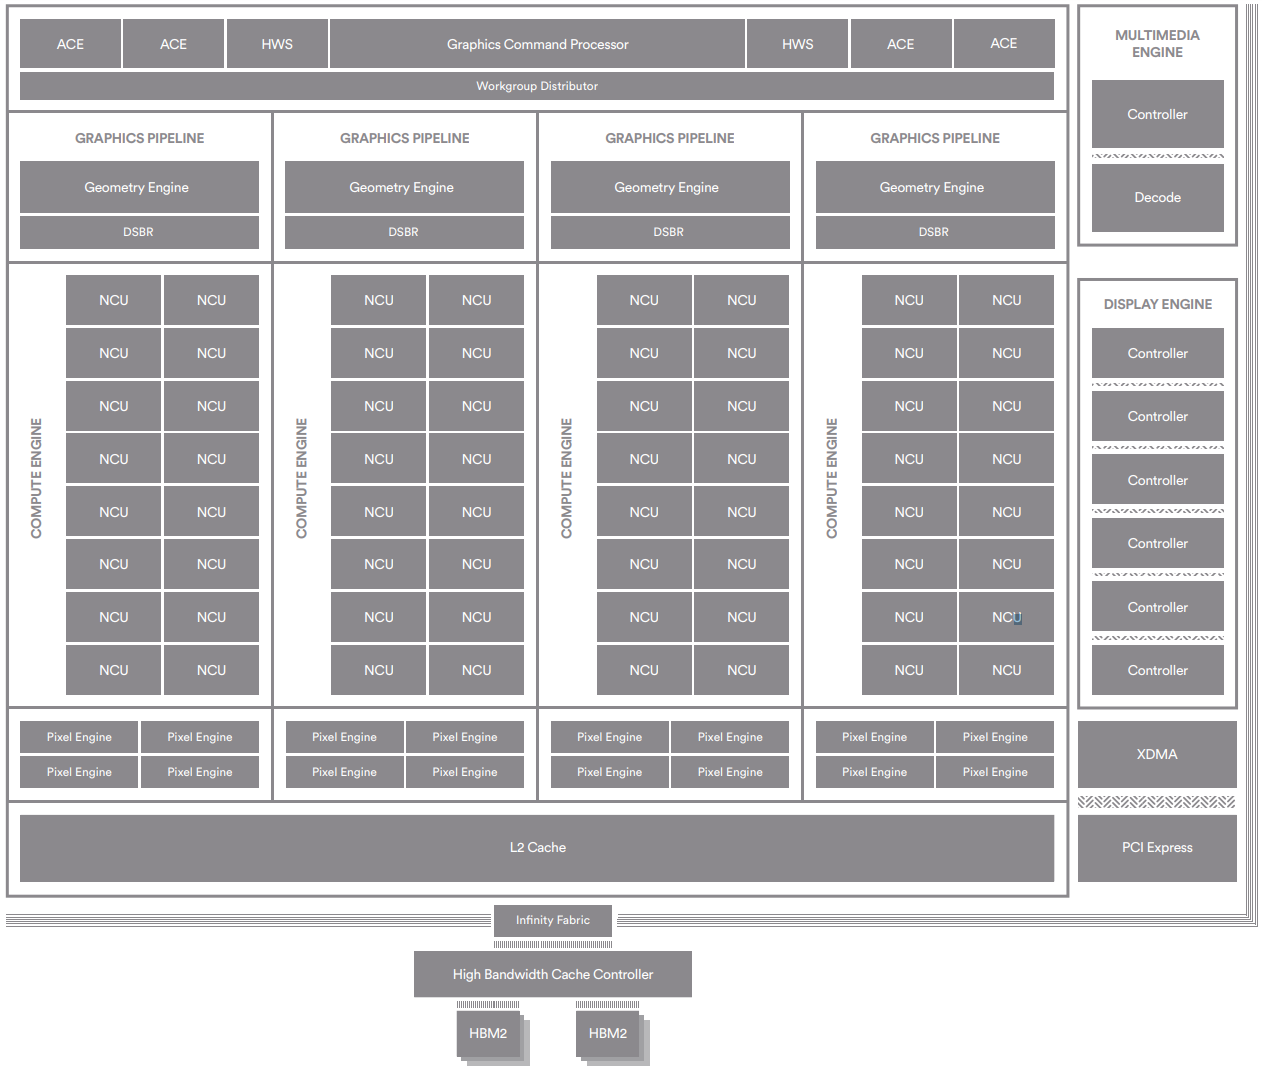
\includegraphics[width=0.7\linewidth]{Figures/Background/Vega10_microarchitecture.png}}
    \subfigure[NCU]{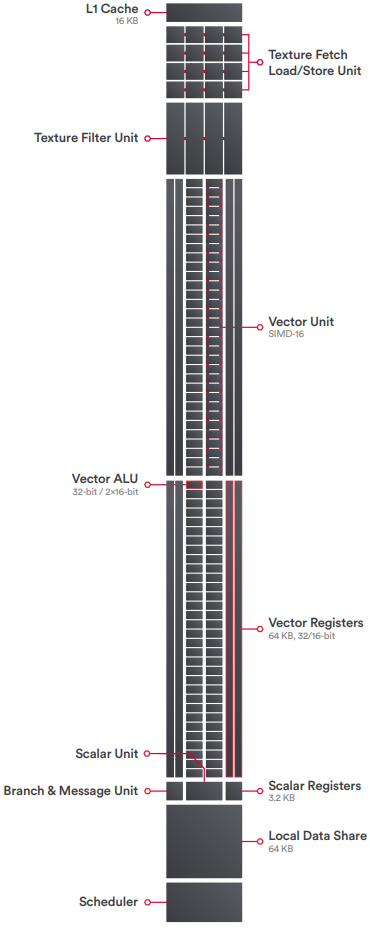
\includegraphics[width=0.24\linewidth]{Figures/Background/NCU.png}}
  \end{subfigmatrix}
  \caption{AMD's Graphics Core Next logical organization.}
  \label{fig:Vega10arch}
\end{figure}


As it was referred before, one of the significant benefits of \acrshort{gpu}s is, the ability to concurrently execute multiple threads. To accomplish for that, each \acrshort{sm} or \acrshort{cu} is made up of hundreds of execution units. However, to manipulate such number of threads, it is necessary to have a significantly large and fast memory system, not only to save the context of each thread, but also to provide low-overhead context switching between the different sets of threads being executed. In that sense, modern \acrshort{gpu} architectures include a large register file on each \acrshort{sm}/\acrshort{cu}. For reference, in the AMD GNC architecture, each \acrshort{cu} has 49,152 (32-bit) registers~\cite{jing_energy-efficient_2013}.

In terms of memory, both the AMD and the NVIDIA \acrshort{gpu}s present a 3 level hierarchy system: a global memory, accessible by all \acrshort{sm}/\acrshort{cu} (generally referred to as video memory); a shared memory associated to each \acrshort{sm} or \acrshort{cu}, accessible by the threads running on that \acrshort{sm} or \acrshort{cu}; and a set of read-only caches for constants and textures, specific to each execution unit.

A \acrshort{gpu} device from AMD will be used to conduct the experimental part of this dissertation. For that reason, the terminology used by AMD will be adopted herein. However, the presented work is independent of the hardware and terminology itself, and could equally be applied to NVIDIA \acrshort{gpu}s.

\subsection{GPU programming model}

The development of CUDA~\cite{nvidia_cuda_2017} (by NVIDIA) and OpenCL~\cite{noauthor_opencl_2013} (by Khronos Group) were the driving force to using \acrshort{gpu}s in general programming. CUDA and OpenCL are both parallel computing platforms and application programming interfaces (\acrshort{api}) that allow developers to create \acrshort{gpu}-accelerated applications, splitting the computations between the \acrshort{cpu} and \acrshort{gpu}. The first versions of these frameworks treated the \acrshort{gpu} as an accelerating slave device, providing a set of directives that allow the \acrshort{cpu} (master device) to transfer data, synchronize and control the \acrshort{gpu}.  Though, to take full advantage of the \acrshort{gpu} architecture and create a true heterogeneous system, the \acrshort{cpu} and \acrshort{gpu} have to collaborate more efficiently. The creation of the Heterogeneous System Architecture (\acrshort{hsa}) \cite{hwu_heterogeneous_2015} framework acts on improving this problem by acting as a low-level intermediary \acrshort{api} to provide improved coordination and communication for heterogeneous computing systems.  More recently, AMD introduced the Radeon Open Computing platform (\acrshort{roc}) \cite{noauthor_radeonopencompute/rocm_2019}. Like CUDA and OpenCL, \acrshort{roc} provides a set of tools that allow developers to create heterogeneous applications. Being a newer software stack, already built on the notions and added benefits of \acrshort{hsa} runtime \acrshort{api}, ROC allows the use of a wider set of programming frameworks like OpenCL, HC++, and HIP.

This programming model is rather similar across the different platforms, with developers traditionally programming the \acrshort{gpu}s using general-purpose languages like C, C++ and Fortran. More recently, the manufacturers are also starting to provide direct access to the \acrshort{gpu} through higher-level languages like Python\footnote{https://developer.nvidia.com/how-to-cuda-python}, allowing for an easier development and adoption of \acrshort{gpu}s as accelerating devices.

Overall, when executing a program on \acrshort{gpu}s, using either of the previously mentioned platforms, a Kernel is invoked on the \acrshort{gpu}, that will execute across several parallel threads. Following this work split, the frameworks expose three levels of abstraction: \textit{threads}, \textit{thread blocks} and  \textit{block grid}. The number of \textit{threads} to be executed can be explicitly defined by the programmer, or implicitly set by the compiler. The \textit{threads} are grouped in \textit{thread blocks} containing an amount of \textit{threads}, and the \textit{thread blocks} are in turn arranged in a \textit{block grid}. When the Kernel is executed, the scheduler maps each \textit{thread block} onto a \acrshort{cu}. Due to this mapping, \textit{threads} within a \textit{thread block} are able to communicate over the \acrshort{cu} shared memory and their execution is synchronized through programable directives.

During the execution of each \textit{thread}, an identifier presents the location of the running \textit{thread} within the \textit{thread blocks} - \texttt{ThreadIdx} and within the \textit{block grid} - \texttt{BlockIdx}. The \textit{thread block} size can be obtained with the \texttt{BlockSize} directive. 

%%%%%%%%%%%%%%%%%%%%%%%%%%%%%%%%%%%%%%%%%%%%%%%%%%%%%%%%%%%%%%%%%%%%%%%%
\section{CMOS Circuit Characterization}
\label{section:CMOS}

For the last 40 years, \acrshort{cmos} (Complementary metal-oxide-semiconductor) has been the most used technology in the creation of digital circuits and processors in general [REF]. 

There are two defined logic levels in digital circuits: logic level $0$ and $1$, each represented by an analog voltage range. To ensure its operations, the circuit requires a DC voltage value $V_{DD}$. The logic gates are excited through an input voltage $V_{i}$ and an output voltage $V_o$, corresponding to the logic level resulting from their logic function (see Figure~\ref{fig:cmos}). As it is illustrated in Figure~\ref{fig:cmos_noise_margin}, the voltage range at the input of the logic gates is correctly interpreted if it falls inside a given range. Logic level $0$ corresponds to the interval between $GND$ ($0V$) to $V_{IL}$, while logic level $1$ corresponds to the interval between $V_{IH}$ to $V_{DD}$. In turn, the output is considered $0$ if it goes from $GND$ ($0V$) to $V_{OL}$ and logic level $1$ from $V_{OH}$ to $V_{DD}$. The limits of the input and output logic levels depend on the intrinsic characteristics of the transistors, such as their dimensions and transconductance values. In addition to the transistors characteristics and operating voltage, any digital circuit is also characterized by their frequency of operation.

\begin{figure}[htb]
    \centering
    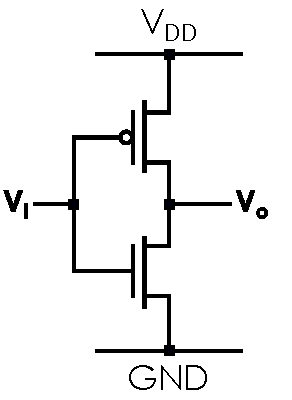
\includegraphics[width=30mm]{Figures/Background/cmos_inverter.pdf}
    \caption{CMOS inverter.}
    \label{fig:cmos}
\end{figure}

\begin{figure}[htb]
    \centering
    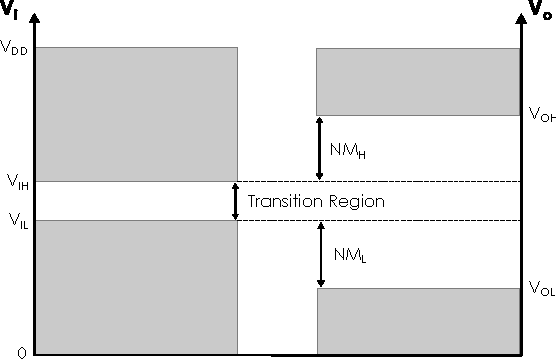
\includegraphics[width=85mm]{Figures/Background/voltage_margin.pdf}
    \caption{Noise margin definitions: $NM_L=V_{IL}-V_{OL}$ and $NM_H=V_{OH}-V_{IH}$.}
    \label{fig:cmos_noise_margin}
\end{figure}

The remaining of this section provides an introduction to the effects of voltage and frequency scaling on the transistor and circuit level operation.

% Moore's law predicted the doubling of the transistors counts roughly every two years. The increase in the number of devices per chip directly translates to the observed performance increase over the last 60 years. However, in the last ten years, the industry is experiencing a slowdown. The shrinking of transistors is harder and harder and the amount of power created by today's chips is limits the transistor count (for the same node size). In this regard, it is indispensable that any digital circuit and, processors in particular, are develop taking into account the underlaying fabrication technology characteristics in order to find new ways of tackling this issues.

% The fundamental solution followed nowadays acts on varying the frequency and voltage values of the CMOS circuit accordingly to what is happening on the device. However, to take fully advantage of these parameters, it is critical to understand the impact of these variations on CMOS circuits.



\subsection{Propagation delay and circuit critical path}

The propagation delay of a logic gate (e.g., inverter) corresponds to the time interval (calculated at $50\%$ of low/high transition) between the application of an input signal and corresponding output switching, as illustrated in Figure~\ref{fig:tp}. Considering both transitions low to high and high to low, the logic gate propagation time ($tp$) corresponds to the average value of the two propagation delays, as defined in Equation~\ref{eq:tp_avg}.

\begin{figure}[htb]
    \centering
    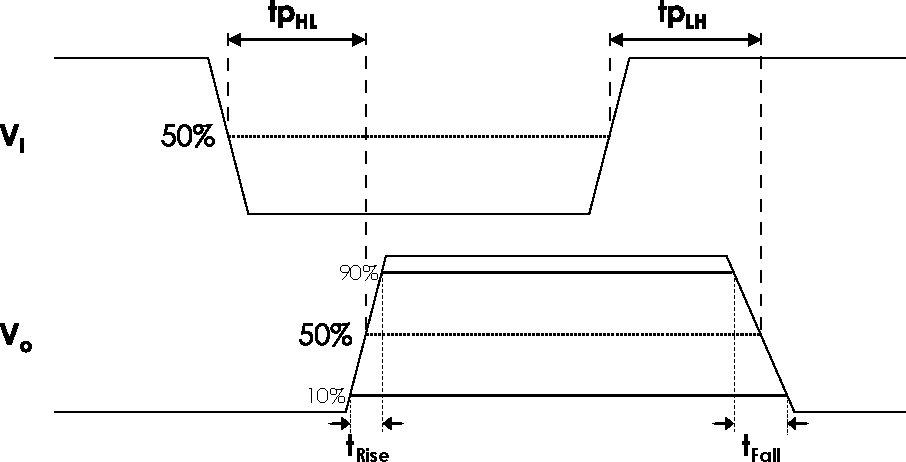
\includegraphics[width=80mm]{Figures/Background/propagation_delay.pdf}
    \caption{Logic gate propagation delay: $tp_{HL}$ - propagation delay high to low; $tp_{LH}$ - propagation delay low to high.}
    \label{fig:tp}
\end{figure}

\begin{equation}
    tp = tp_{avg} = \frac{tp_{HL}+tp_{LH}}{2}
    \label{eq:tp_avg}
\end{equation}

This metric is related to the time that the logic gate takes to switch its output logic level ($t_{Fall}$ for the high to low transition and $t_{Rise}$ for the low to high transition). This transition can be modeled as a first-order RC circuit (see Figure~\ref{fig:rc_circuit}) with the transient response following Equation~\ref{eq:firtst_order}, where $\tau$ corresponds to the time constant. This time constant reflects the intrinsic characteristics of the transistors that make up the logic gate, being $\tau=RC$, where $R$ represents the average output resistance of the transistor when it is turned 'ON' and $C$ the output capacitance that the logic gate is driving.


\begin{figure}[htb]
    \centering
    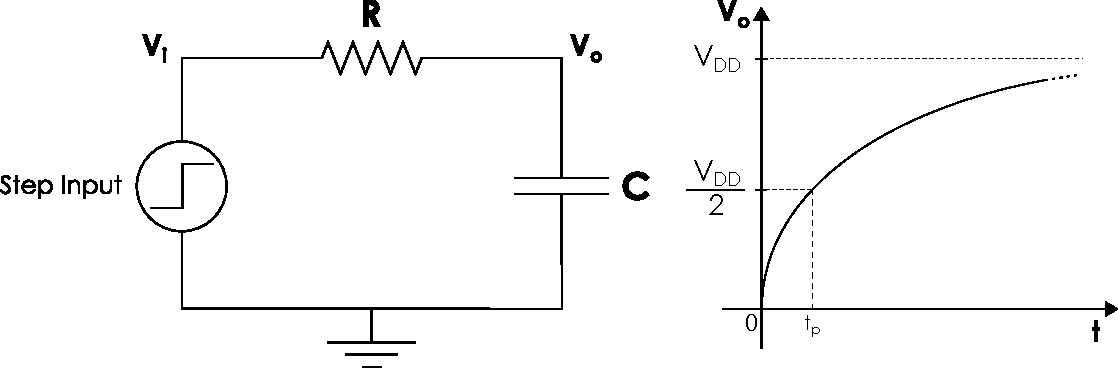
\includegraphics[width=105mm]{Figures/Background/rc_circuit.pdf}
    \caption{First order RC circuit and its corresponding temporal response to step input.}
    \label{fig:rc_circuit}
\end{figure}

\begin{equation}
    V_o=V_{DD} \cdot (1-e^{-t/\tau})
    \label{eq:firtst_order}
\end{equation}

By solving Equation~\ref{eq:firtst_order} for $V_o=\frac{V_{DD}}{2}$, it is observed that the propagation delay is a function of the supplied voltage, of $R$ and $C$, as depicted in Equation~\ref{eq:tp}.


\begin{equation}
    t_p=-ln\left(1-\frac{V_{DD}}{2 \cdot V_{DD}}\right)\cdot\tau=-ln(0.5)\cdot\tau=ln(2)\cdot\tau
    \label{eq:tp}
\end{equation}


From all the logic paths (sequence of logic gates) that connect any two registers, the one which presents the largest sum of the propagation delay limits the overall maximum frequency that the \acrshort{cmos} circuit can operate, establishing itself as the critical path of the circuit (see Figure~\ref{fig:critical_path}). However, in the particular case of a microprocessor circuit, depending on the operation (instruction) being performed (and so, of the used architectural component), the circuit's critical path can change.

\begin{figure}[htb]
    \centering
    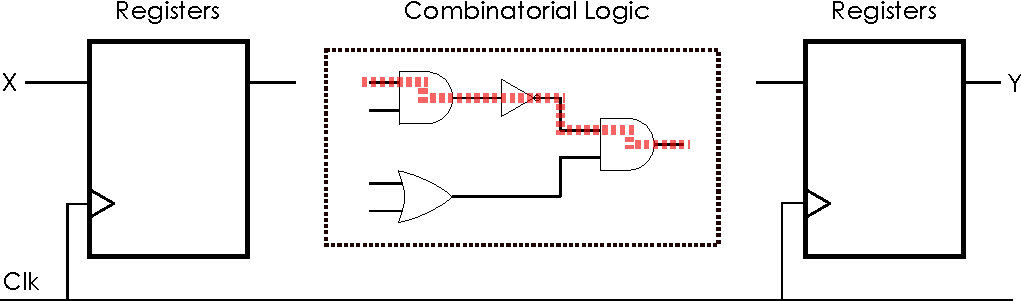
\includegraphics[width=130mm]{Figures/Background/comb_logic.pdf}
    \caption{Critical path between two registers (red dashed line).}
    \label{fig:critical_path}
\end{figure}

In this way, when scaling the circuit's operating frequency, it is only possible to increase it until it matches the inverse of the critical path propagation delay. When raising the frequency ahead of this value, the critical path is violated, meaning that when the next clock cycle starts, the output of the combinatorial logic may not be the correct one.

% When manufacturers set the digital circuit's operating frequency, they never go up to the maximum possible frequency, leaving a safe operating margin. This margin exists to guarantee correct and safe operation under process, voltage and temperature (\acrshort{pvt}) variation.



\subsection{Voltage guardband, PVT Variation and Aging}

After the release of the digital circuit, silicon vendors often deal with variations of their devices' specifications. On the design stage of the circuit, these variations need to be correctly predicted and accounted for, guaranteeing the correct operation of the circuit throughout time and range of conditions that the circuit will be exposed to.

Process, voltage and temperature (\acrshort{pvt}) variation and aging impact the circuit in different manners and the solution for all is to put in place a voltage guardband, as defined in Figure~\ref{fig:voltage_guardband}. This voltage guardband increases the circuit nominal voltage from the best-case operating voltage selected from the transistors and gates' intrinsic characteristics.
In Equation~\ref{eq:tp}, the propagation delay is now obtained by considering the ratio between the best-case operating voltage\footnote{(Threshold voltage) and the considered supply voltage}. Hence, when the silicon vendor opts to put in place a voltage guardband, increasing the supplied voltage (overvoltage), the propagation delay will follow Equation~\ref{eq:tp_v_scaling}, where $V_{Threshold}$ depends on the transistors (and so, it does not depend on the supply voltage value) and $V_{Supply \: Voltage}$ is the supplier controlled parameter. Figure~\ref{fig:voltage_scaling} illustrates the logic gate step response for over and undervoltage. Increasing the supply voltage will make the transistors switch faster, while decreasing it, reduces the switching pace.



\begin{equation}
    t_p=-ln \left( 1-\frac{V_{Threshold}}{V_{Supply \: Voltage}}\right)\cdot\tau=ln\left(\frac{2V_{Supply \: Voltage}}{2V_{Supply \: Voltage}-V_{Threshold}}\right)\cdot\tau
    \label{eq:tp_v_scaling}
\end{equation}

\begin{figure}[!htb]
    \centering
  \begin{subfigmatrix}{2}
    \subfigure[Voltage guardband definition.]{
    \centering
    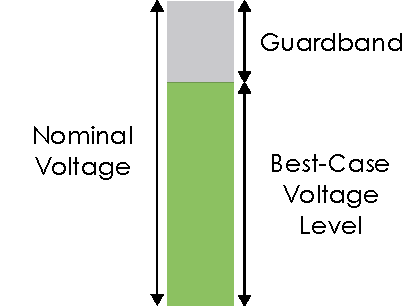
\includegraphics[height=4cm]{Figures/Background/voltage_guardband_bar.pdf}
    \label{fig:voltage_guardband}}
    \subfigure[First order circuit step response when changing the supply voltage ($V_{sv}$).]{
    \centering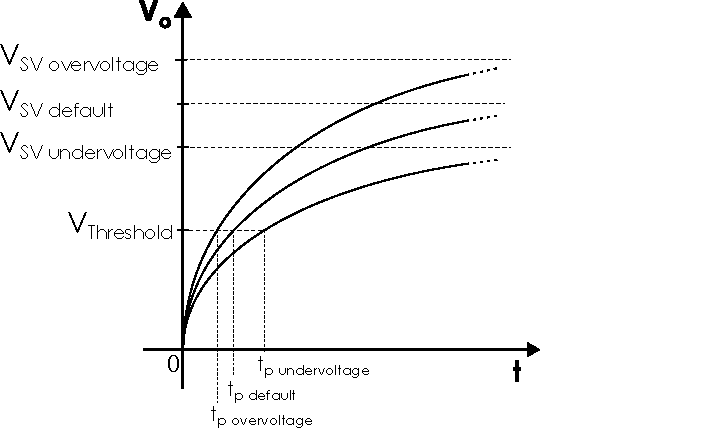
\includegraphics[height=7cm]{Figures/Background/v_scaling.pdf}
    
    \label{fig:voltage_scaling}}
  \end{subfigmatrix}
  \caption{Voltage guardband ensures reliability by making the transistors switching faster.}
\end{figure}




\subsubsection{Process variation and aging}

Process variation and aging impact the circuit in different ways. Process variation is related to the modern fabrication process of silicon. It results from imperfections in the lithography and dopant diffusion, affecting the transistors' dimensions (for example, length and oxide thickness). This dimensionality change between the transistors can occur either intra-die, when devices from the same die present different features depending on their locations, and inter-die, meaning that devices from one die can present different traits from devices from another batch of dies. The process variation affects the speed of transistors and the overall circuit characteristics, by varying the device voltage threshold and speed \cite{schemmert_threshold-voltage_1974, thomas_core_2016}. Such variations are inherent to the fabrication process. Even though silicon manufacturers try to reduce this impact, such variation will always occur as a \textit{static} variation after the release of the chip to the market.

Aging of the \acrshort{cmos} circuits is a result of ongoing chip temperature variation and supply voltage change. The continuous variation of these two factors induces \textit{Bias Temperature Instability} (\acrshort{bti}) and  \textit{Hot Carrier Injection} (\acrshort{hci}). \acrshort{bti} causes threshold voltage shifts over long periods due to the presence of voltage stress at the transistors' gate. On the other side, \acrshort{hci} is caused by the acceleration of carriers (electrons/holes) under lateral electric fields in the channel of MOS devices. The acceleration can get up to the point where the carriers gain enough energy and momentum to cause damage, degrading mobilities and again, changing the threshold voltages~\cite{sapatnekar_what_nodate}.

The occurrence of these phenomenons raises the possibility of the circuit diverge from its original specifications. Hence, a circuit that is dimensioned without any headroom (not sufficiently large voltage guardband) may not be able to cope with such a process variation - producing a not working circuit; or stopping to work overtime due to aging.



\subsubsection{Voltage variation}

As it was previously observed, running the circuit at an increased voltage compared to the required voltage at the target frequency for typical workloads results in a faster circuit. This increment in performance allows for inserting an extra timing margin in each clock cycle, as described in Figure~\ref{fig:timming_guardband}. 

\begin{figure}[!htb]
  \begin{subfigmatrix}{2}
    \subfigure[Static Margin]{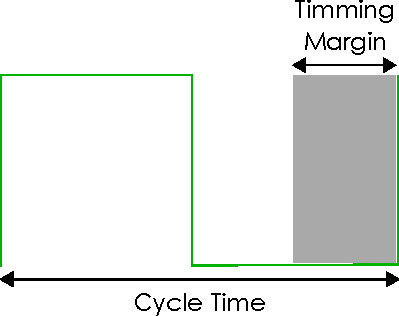
\includegraphics[height=4.5cm]{Figures/Background/static_margin.pdf}}
    \subfigure[Reduced Voltage Margin]{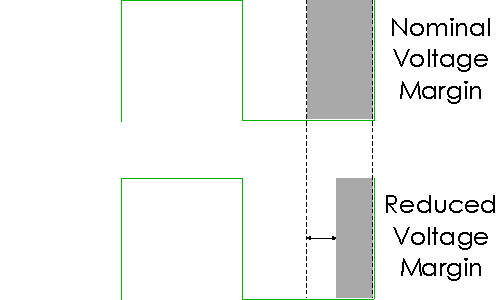
\includegraphics[height=4.5cm]{Figures/Background/reduced_voltage_margin.pdf}}
  \end{subfigmatrix}
  \caption{Voltage guardband ensures operation reliability by effectively inserting some extra timing margin.}
  \label{fig:timming_guardband}
\end{figure}

This timing margin is of extreme importance to cope with voltage noise, the leading cause of voltage variation during the circuit execution. Voltage noise is mainly induced by $di/dt$ droop. This phenomenon makes the actual measured voltage that is  applied to the circuit components (as formulated in Equation \ref{eq:Vactual}), depend on the rate of change of the current being drawn. 

\begin{equation}
    \label{eq:Vactual}
    V_{actual} = V_{DD}-L*\frac{di}{dt}
\end{equation}

The runtime workload intensity variation induces the $di/dt$ droop due to the rapid and significant change in current demand from the various circuit functional blocks~\cite{thomas_core_2016}. Thus, in the case of processors, the workload type can directly impact voltage noise. As a result, a program that induces a bigger $di/dt$ droop will need to have a bigger voltage guardband.

\subsubsection{Temperature variation}

Temperature variation occurs both due to changes on the environmental temperature, and due to changes in the temperature that is dissipated as heat by the transistors on the circuit. The temperature affects the transistors by changing the carriers' mobility ($ \mu [\frac{cm^2}{V\cdot s}]$), and threshold voltage ($V_t$)\cite{wolpert_temperature_2012}.

The carriers' mobility $ \mu $ describes the drift velocity of a particle in an applied electric field, thus the transistor's capability to drive electric current. Usually, the carrier mobility of MOS transistors presents a very complex temperature dependence. However, in general, the mobility is said to decrease with temperature increase. 

In the case of threshold voltage, its rate of change also follows the same principle of the carriers mobility. However, it usually has a more straightforward dependency of decreasing linearly with temperature increase.

The work of Freijado \textit{et al.}~\cite{freijedo_modeling_2012} presents a model that tries to encompass all these variations and test the impact that temperature has on the propagation delay. The designed model predicts that the propagation delay increases linearly with the temperature increase, which would imply that the size of the voltage guardband reduces when the temperature increases. 

\subsection{Power Consumption}
\label{sec:power_consumption}
On a \acrshort{cmos} circuit, the total consumed power is decomposed into the dynamic and static parts

\begin{equation}
    P_{CMOS} = P_{dynamic} + P_{static}.
    \label{eq:power}
\end{equation}

The dynamic power relates to the power that is consumed by the transistors flipping stages (inverting the logic values), and corresponds to the power of charging and discharging the internal net capacitances. This value is proportional to the frequency that this change occurs. Equation~\ref{eq:dynpower} represents the general formulation of the dynamic power, where $a$ represents the device utilization factor, $C$ the total capacitance of the circuit, $V$ the circuit supply voltage, and $f$ the frequency of operation~\cite{gonzalez_supply_1997}.

\begin{equation}
    P_{dynamic} = aCV^2f
    \label{eq:dynpower}
\end{equation}

On the other hand, the static part of the power consumption comprehends three components: $P_{leakage}$, $P_{short-circuit}$ and $P_{DC}$~\cite{mei_survey_2016}. The leakage power is independent of the transistors flip, and it represents the flow of electrons between the transistors' source, drain, and gate, known as leakage current. The short-circuit power comes from the instantaneous short-circuit connection between the supply voltage and the ground when the transistor flips. Finally, the Direct Current (DC) power corresponds to the power needed for powering the circuit. Equation \ref{eq:cmosstatic} represents the expression with all static power consumption components.

\begin{equation}
    P_{static} = P_{leakage} + P_{short-circuit} + P_{DC}
    \label{eq:cmosstatic}
\end{equation}

Usually, the dynamic power dominates the total power consumption of a circuit. However, with the current tendency to reduce the manufacturing size of transistors, the static power is becoming a more significant part \cite{s._hong_modeling_2012,hong_integrated_2010}. Nevertheless, as a common reference, and due to the usually dominant weight of the dynamic power on the total power consumption, the power used by a \acrshort{cmos} circuit usually changes linearly with the clock frequency and quadratically with the supplied voltage.


%%%%%%%%%%%%%%%%%%%%%%%%%%%%%%%%%%%%%%%%%%%%%%%%%%%%%%%%%%%%%%%%%%%%%%%%
\section{Dynamic Voltage and Frequency Scaling}
\label{section:DVFS}

The widespread use of \acrshort{gpu}s in both supercomputers and personal computing machines comes at the cost of a significant increase in power consumption. While a typical modern CPU consumes about 50 to 100W, it is common to see \acrshort{gpu}s consuming between 200 and 300W of power. With these figures, the use of energy efficiency techniques to try to reduce power consumption becomes a vital issue.

As stated in Section~\ref{sec:power_consumption}, the power consumption of a \acrshort{cmos} circuit increases linearly with the operating frequency and quadratically with the supplied voltage. Thus, a direct manner of reducing this figure is by directly acting on these two parameters. 
Dynamic Voltage and Frequency Scaling (\acrshort{dvfs}) is a power management technique which performs "on the fly" control of frequency and voltage. \acrshort{dvfs} allows for an energy efficiency improvement by matching the \acrshort{gpu} utilization to voltage and frequency settings. When the \acrshort{gpu} is idle, the frequency is lowered, and when it is active, the frequency is increased. As presented in the previous section, the frequency scaling also implies a change in voltage to accommodate the critical path timing constraints' fulfillment. 

In general, the applied voltage level $V$ is a function of the current operating frequency $f$, in the form of $V(f)$. Therefore, by intelligently controlling the clock frequency, the required voltage level for stable operation of the circuit can also be reduced, leading to further power savings.

In general, modern \acrshort{gpu} boards have independent control over two pairs of frequency and voltage. Each pair (or domain) acts on a distinct part of the \acrshort{gpu}, intending to maximize the performance or reduce the power consumption. The first domain concerns the \acrshort{gpu} core, acting on all \acrshort{sm}/\acrshort{cu}s, the cache, and the interconnection fabric. The second affects the \acrshort{dram} chips that compose the video memory. 

The clock frequency is an independently controlled variable, and its change directly reflects on the performed achieved by the \acrshort{gpu}. An increase in the clock frequency of the core results in an improvement of the \acrshort{sm}/\acrshort{cu} execution speed, while the same change in the memory frequency will increase the \acrshort{dram} I/O throughput \cite{mei_survey_2016}. The voltage level of each domain is dependent on the clock frequency being computed based on tests performed by the manufacturer to ensure the correct operation of the circuit, independently of the workload.

The two major \acrshort{gpu} silicon vendors, AMD and NVIDIA, have on their products the concept of performance levels. A performance level is a pair of frequency and voltage that can be applied to the \acrshort{gpu} \acrshort{dvfs} domains. These vary from low power and performance levels to high performance and high power ones. The idea of having multiple performance levels is to be able to always be at the best point of operation. In the case of the first \acrshort{gpu} (AMD Vega 10 Frontier Edition) that is going to be used in the experimental phase of the dissertation, the \acrshort{gpu} core has eight performance levels, while the memory has only four. Table \ref{tab:gpulevels} shows the reference values for frequency and voltage for each of the core and memory performance levels. 
The increase of frequency observed at the higher performance levels is, as expected, accompanied by the increased voltage to accommodate the frequency boost.


\begin{table}[!htb]
\renewcommand{\arraystretch}{1.2} % more space between rows
\centering
\begin{tabular}{ccclccc}
\multicolumn{3}{c}{\textbf{Core}}                                         & \multicolumn{1}{c}{\textbf{}} & \multicolumn{3}{c}{\textbf{Memory}}                                             \\
\textbf{Level} & \textbf{Frequency {[}MHz{]}} & \textbf{Voltage {[}mV{]}} &                               & \textbf{Level}       & \textbf{Frequency {[}MHz{]}} & \textbf{Voltage {[}mV{]}} \\ \cline{1-3} \cline{5-7} 
0              & 852                          & 800                       &                               & 0                    & 167                          & 800                       \\
1              & 991                          & 900                       &                               & 1                    & 500                          & 900                       \\
2              & 1138                         & 950                       &                               & 2                    & 800                          & 950                       \\
3              & 1269                         & 1000                      &                               & 3                    & 945                          & 1000                      \\ \cline{5-7} 
4              & 1348                         & 1050                      &                               & \multicolumn{1}{l}{} & \multicolumn{1}{l}{}         & \multicolumn{1}{l}{}      \\
5              & 1440                         & 1100                      &                               & \multicolumn{1}{l}{} & \multicolumn{1}{l}{}         & \multicolumn{1}{l}{}      \\
6              & 1528                         & 1150                      &                               & \multicolumn{1}{l}{} & \multicolumn{1}{l}{}         & \multicolumn{1}{l}{}      \\
7              & 1600                         & 1200                      &                               & \multicolumn{1}{l}{} & \multicolumn{1}{l}{}         & \multicolumn{1}{l}{}      \\ \cline{1-3}
\end{tabular}
\caption{GPU Core and Memory Levels of Frequency and Voltage - AMD Vega 10 Frontier Edition}
\label{tab:gpulevels}
\end{table}


Newer \acrshort{gpu} \acrshort{dvfs} systems, like the one used on the second \acrshort{gpu} under test (AMD Radeon 5700 XT) improve the number of performance levels by allowing for a continuous used of all frequency values within the valid range (versus discretizing the domain into a set number of performance levels). In this case, there are three user-defined frequency-voltage pairs on which a quadratic regression is computed  (see Figure~\ref{fig:voltage_curve}), creating a $f(V)$ function that for every frequency, gives the correspondent voltage value.

\begin{figure}[htb]
  \centering
  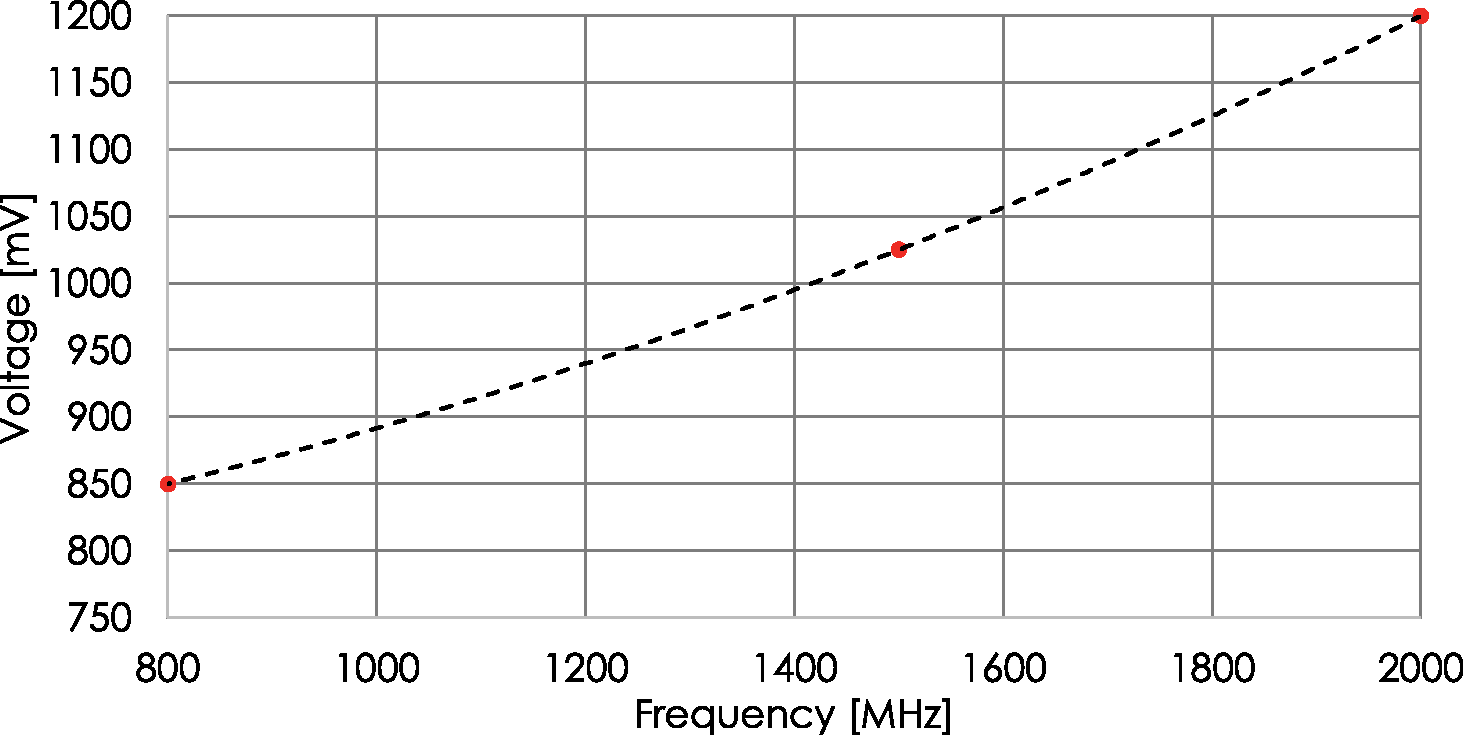
\includegraphics[width=0.75\textwidth]{Figures/Background/voltage_frequency_curve.pdf}
  \caption{GPU Core voltage frequency curve, red dots indicate the default user-defined voltage frequency pair - AMD Radeon 5700 XT.}
  \label{fig:voltage_curve}
\end{figure}

\subsection{Control Mechanism}

The correct choice of the most appropriate performance level for each \acrshort{gpu} \acrshort{dvfs} domain when executing a given application is one of the topics with more research from both manufacturers and researchers. The correct design of the \acrshort{dvfs} controller has a significant impact on the \acrshort{gpu}'s performance and energy efficiency.

The first implementations of \acrshort{gpu} \acrshort{dvfs} controllers took direct inspiration from the \acrshort{cpu} \acrshort{dvfs} and can be largely classified into interval-based, inter-task, and intra-task \acrshort{dvfs} algorithms~\cite{boyer_improving_2013}. 

\subsubsection{Interval-based}

Interval-based algorithms rely on the periodical measurement of the device's utilization, setting the next frequency and voltage based on the average measurement of utilization. The utilization $U_{i}$ reflects the percentage of working time, $w_{i}$, spent by the \acrshort{gpu} over the last time frame $TF_{i}$ and can be formulated using equation \ref{eq:utilization}.

\begin{equation}
    U_i=\frac{w_i}{TF_i}
    \label{eq:utilization}
\end{equation}

By applying arithmetic, geometric, weighted average, or a more complex algorithm, over the last $n$ $U_{i}$ measurements,  the next utilization $U_{i+1}$ is predicted. If the predicted value surpasses pre-determined upper or lower thresholds, the frequency is adjusted up or down accordingly \cite{seongki_gpgpu-perf:_2015}. 
A \textit{governor} is a set of parameters (such as frequency and voltage tables), thresholds and a utilization prediction algorithm that controls how the interval-based \acrshort{dvfs} works. By choosing a different \textit{governor}, the \acrshort{dvfs} system can react differently to the same workload. Figure \ref{fig:DVFSprocedure} schematizes the periodic procedure executed by the \acrshort{dvfs} system~\cite{seongki_gpgpu-perf:_2015}. 

\begin{figure}[htb]
  \centering
  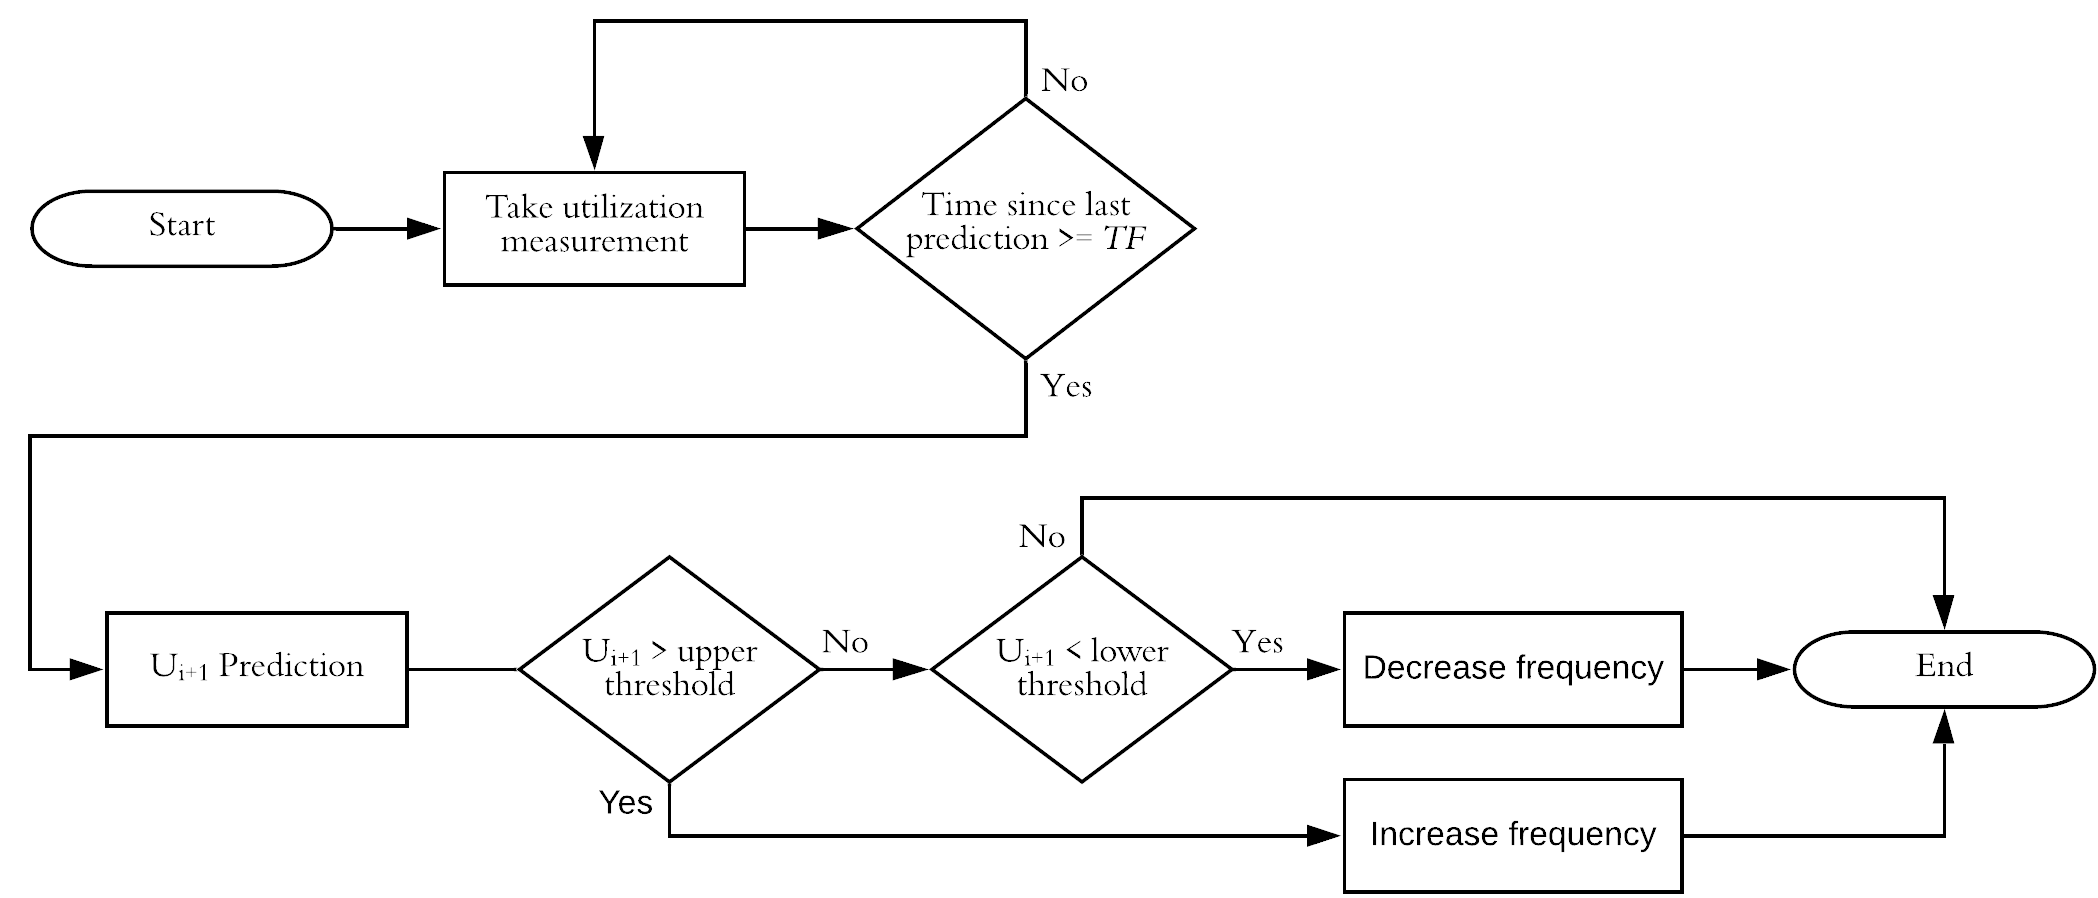
\includegraphics[width=\textwidth]{Figures/Background/DVFSprogram.png}
  \caption{Interval-based DVFS procedure.}
  \label{fig:DVFSprocedure}
\end{figure}

\subsubsection{Task-based}

Task-based \acrshort{dvfs} algorithms analyze the program source code, and past runs profiling results to determine the optimal frequency/voltage for each task. This type of algorithm is composed of an intra-task and an inter-task analysis \cite{noauthor_time_nodate}. The intra-task part decomposes the process execution into the on-chip computation and off-chip access latencies. Based on the results,  the optimal \acrshort{gpu} core and memory frequencies are determined accordingly to the ratio between the two types of execution. Inter-task mechanisms utilize the intra-task results, assigning a signature to each type of task/process. By analyzing, in run-time, the \acrshort{gpu} components' utilization, and using a lookup table that stores the signatures, the optimal frequency/voltage is selected for the sequence of tasks to be executed.

\bigskip
In general, the challenges of creating a better \acrshort{gpu} \acrshort{dvfs} relates to three factors. \acrshort{gpu} power management is minimal, lack of accurate quantitative \acrshort{gpu} \acrshort{dvfs} performance and power estimation tools, and the \acrshort{gpu} architecture design is still evolving rapidly, which makes the strategies applied to one architecture design have different outcomes on the next iteration of it \cite{mei_survey_2016}. The observed results show that strategies like scaling up the processor frequency, race-to-idle  \cite{hoffmann_racing_2013} or "racing" \cite{kim_racing_2015}, when a task is launched in the pursuit of finishing it as fast as possible and return to an idle state, prof to increase the energy efficiency of CPUs. However, that assumption not always results in the same outcome for \acrshort{gpu}s \cite{kim_racing_2015}. 

\subsubsection{AMD/NVIDIA DVFS Mechanism Example}

The \acrshort{gpu} \acrshort{dvfs} control mechanism used nowadays by both AMD and NVIDIA, schematized on figure \ref{fig:DVFSmechanism}, is primarily an interval-based one. The most recent AMD \acrshort{gpu} \acrshort{dvfs} mechanism is called Adaptive Frequency and Voltage Scaling (\acrshort{afvs}) \cite{amd_polaris_2017}. \acrshort{afvs} takes into account the voltage levels across the different parts of the \acrshort{gpu}, the die temperature, the desired frequency and the total power consumption. The controller's objective is to maintain the total power consumption within the required power and temperature envelope. Upon launching a new task and within a set power target, the \acrshort{gpu} tries to achieve the highest possible frequency (highest performance level). For that frequency configuration, it also adjusts the voltage level to the one required to correct functioning. With the highest performance level, power and temperature will increase, when one of these parameters achieves the limit, the \acrshort{gpu} decreases to a lower performance level to maintain itself within the power and temperature target. 

\begin{figure}[htb]
  \centering
  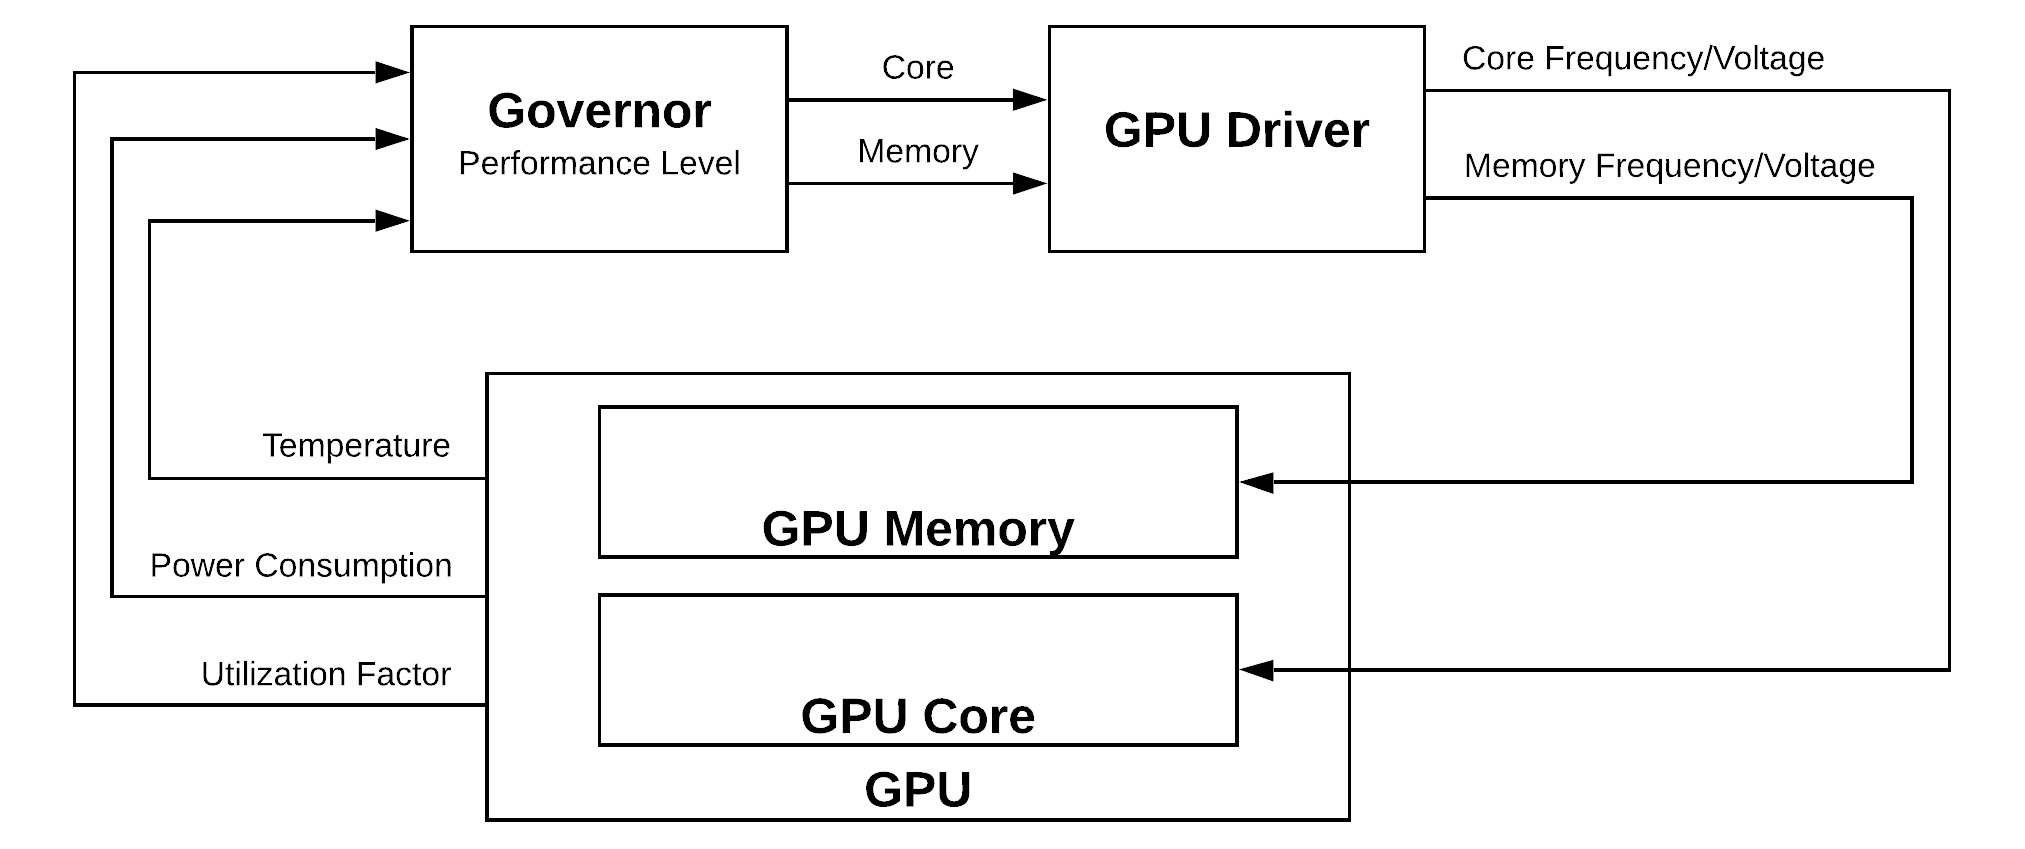
\includegraphics[width=0.8\textwidth]{Figures/Background/DVFS.png}
  \caption{AMD/NVIDIA DVFS control mechanism.}
  \label{fig:DVFSmechanism}
\end{figure}

The major drawback of current \acrshort{gpu} \acrshort{dvfs} implementations is not taking into account the type of task that the \acrshort{gpu} is solving. The dominant control mechanism still considers the \acrshort{gpu} as a black box and controls its \acrshort{dvfs} settings by only looking at outside parameters. Even though such a black-box approach enables significant improvements in current hardware, it lacks the optimization of the frequency/voltage to the type of workload. For instance, a given application can be compute-bound or memory-bound, depending on if the time that it takes to perform the task is limited by the processor performance or the memory bandwidth and latency. This binary classification of applications also depends on the frequency of the core and memory. The same application can be compute-bounded at a low core frequency but be memory-bounded at a higher one \cite{guerreiro_dvfs-aware_2019} (the bottleneck switches from the processing elements to the memory). In the case of a compute-bounded application, the limitation can be imposed by different components of the processor architecture, depending on the type of data (integer or floats) and the intended precision (size of the operands). If one compares the computation with the same type of operands, but with different precision (for instance, 16 vs. 32 bits), even though the \acrshort{gpu} uses the same arithmetic unit, the critical path for 32 bits operands is of increased length. That is the maximum delay between the input and the operations output increases with the operands' precision. 
Since no information about the application is provided to the \acrshort{dvfs} controller, no adaptation of the V-F settings can be employed.
Considering that the manufacturers do not tune their devices to the minimum voltage level (to accommodate for manufacturing imprecisions and to leave a safe guardband), the operating voltage of the circuits can be significantly reduced, leading to significant power savings. 

Overall, the minimum operating voltage of each performance level is set at a high enough level to ensure the correct functioning of the \acrshort{gpu}, independent of the type of computations/workload. Nevertheless, it is possible to fine-tune the voltage and frequency better if the type of task being executed is known at run-time. A significant limitation of the voltage frequency control system is the time it takes to change and stabilize the intended V-F pair. On the case on the AMD Vega 10 Frontier Edition, the mechanism takes approximately 200-500 ms to change between performance levels.

\subsection{GPU DVFS Characterization}

Since the \acrshort{gpu} is such a widely used computation platform, to improve its performance and energy efficiency, it is significant to characterize and analyze the \acrshort{dvfs} effects, mainly in what concerns the impact of the different parameters on different workload scenarios. 

A complete \acrshort{gpu} \acrshort{dvfs} characterization is explored in the literature using two methodologies. The first refers to experimental studies, where researchers use real \acrshort{gpu}s to perform voltage and frequency scaling. Due to past dominance of NVIDIA over AMD \cite{noauthor_jon_2018, mujtaba_amd_2019} and the fact that this manufacturer only offers limited support for independent voltage scaling tools, the majority of the work act solely on frequency scaling. The second approach uses simulators, like GPGPU-Sim \cite{noauthor_gpgpu-sim/gpgpu-sim_distribution_2019} and GPUWattch \cite{noauthor_gpu_2011, leng_gpuwattch:_2013},  to simulate various scaling approaches like \acrshort{gpu} core number scaling and per-core \acrshort{dvfs} \cite{mei_survey_2016}. The benefit of using simulators over real hardware comes on the increased flexibility, enabling the experimentation of scenarios not supported by the frequency/voltage scaling tools provided by the manufacturers. In both methodologies, the studies act on the impact on performance, energy consumption and overall energy efficiency.

The following subsections present a brief overview of some of these works.


\subsubsection{Experimental Approach}

Jiao \textit{et al.} \cite{jiao_power_2010} scaled the \acrshort{gpu} core and memory frequency of an NVIDIA Tesla GTX 280 using three types of workload: a compute-bounded dense matrix multiplication application; a memory bounded application that performs dense matrix transpose; and a mixed workload, Fast Fourier Transform (FFT) computation. The experimental study showed that for the same core-memory frequency settings, the three applications showed different performance and energy efficiency curves. While a compute bounded application showed to be insensitive to memory scaling, the memory bounded application takes advantage of high memory frequency and low core frequency. At last, the mixed workload FFT application profits from both high core and memory frequency. In general, it was shown that energy efficiency could be determined by the instructions per cycle (IPC) metric and by the global ratio of memory transactions by computation transactions.

Ge \textit{et al.} \cite{ge_effects_2013} explored dense matrix multiplication kernel executions in more detail using an NVIDIA Kepler K20c \acrshort{gpu}.  The work revealed that for this type of kernel (compute-bounded), the \acrshort{gpu}'s power and achievable performance is linear to the \acrshort{gpu} core frequency and that the total power consumption had no relation to frequency scaling. In all the used application tests, the energy efficiency has a linear relation with the \acrshort{gpu} frequency, with the highest energy efficiency achieved when the highest clock frequency was employed.

Abe \textit{et al.} \cite{abe_power_2012} introduced a global scaling procedure that combines the \acrshort{gpu} core and memory frequency with the CPU frequency to minimize energy consumption. The first experiment tried to optimize the computation of dense matrix multiplication with differing matrix sizes. Using this global scheme on a small matrix leads to a 28\% energy saving while using low \acrshort{gpu} memory frequency and high \acrshort{gpu} core frequency. The same procedure was then enlarged to a more diverse set of 33 benchmarks where all the possible combinations of a low, medium, and high \acrshort{gpu} core and memory frequency were tested to find the optimal working settings. It was found that energy consumption can be reduced as much as 75\% with a performance loss of 30\% when the best settings were used. 

Mei \textit{et al.} \cite{mei_measurement_2013} conducted a more general experimentation using 37 \acrshort{gpu} benchmarks. In this work, it was possible to observe that the effect of \acrshort{gpu} \acrshort{dvfs} depends on application characteristics. In all situations, the fine-tuning of \acrshort{dvfs} per application (finding the lowest voltage level for the desired running frequency) conveyed an energy-saving of 20\%, on average, with only a 4\% performance loss. More recently, Mei  \textit{et al.}, expanded the previous work to analyze the relation between energy consumption and dynamic frequency scaling settings \cite{mei_survey_2016}. For the  Rodinia benchmark \cite{che_rodinia:_2009}, it was found that some benchmarks increase the energy consumption linearly with frequency scaling while others are insensitive to the change of this parameter. In the particular case of \acrshort{gpu} memory frequency scaling, the work revealed that underclocking this component can result in a 30\% energy decrease if the running application is not memory bounded. For the case of applications whose performance depends on the memory, decreasing its frequency can lead up to 54\% energy increased, due to the increased execution time. The tested set of applications showed that overclocking the memory results in diminishing execution time with reduced overall energy consumption (the memory energy consumption increase overshadows the small reduction in computation time). 

Overall, the relation between the \acrshort{dvfs} settings and the energy consumption depends heavily on the application type. A simple linear model (normally used by the \acrshort{gpu} manufacturers) for \acrshort{dvfs} settings is inadequate to achieve the best performance or energy consumption/efficiency.

\subsubsection{Simulation}

As it was previously referred, the characterization of \acrshort{gpu} \acrshort{dvfs} with simulation approaches is done by using software tools like GPGPU-Sim \cite{noauthor_gpgpu-sim/gpgpu-sim_distribution_2019} and GPUWattch \cite{noauthor_gpu_2011} \cite{leng_gpuwattch:_2013}. GPGPU-Sim is an architecture simulator of a \acrshort{gpu} architecture running CUDA and OpenCL workloads. GPUWattch is an energy model that predicts energy consumption based on the number of computations and memory access that GPGPU-Sim simulates. Together, both programs can be used to model current and novel \acrshort{gpu} architectures and \acrshort{dvfs} controllers accurately.

Leng \textit{et al.} \cite{leng_gpuwattch:_2013}, the developers of GPUWattch, simulated the execution of compute and memory-bounded kernels in three scenarios: no \acrshort{dvfs} and using a custom off-chip and on-chip \acrshort{dvfs}. The custom \acrshort{dvfs} algorithms monitor the average number of stall cycles caused by memory operations. When the number increases, the controller switches to a slower performance state, whereas the number of stall cycles reduces, the controller places the \acrshort{gpu} in a higher performance level. The difference between the on-chip and off-chip \acrshort{dvfs} techniques is the time that it takes to respond to the number of stall cycles. While the on-chip can switch the performance level in 500 cycles, the off-chip takes 10000 cycles. The experiments show that using the off-chip \acrshort{dvfs} versus no \acrshort{dvfs} results in 13.2\% of energy savings (on average) while using the on-chip \acrshort{dvfs} yield a 14.4\% energy saving.

Cha \textit{et al.} \cite{cha_core-level_2018} used GPGPU-Sim to create a \acrshort{gpu} core space-multitasking simulator, where per-kernel dynamic frequency scaling (acting on the computing unit level) settings can be applied in concurrent kernel execution. They used Rodinia suite \cite{che_rodinia:_2009}, Parboil suite \cite{stratton_parboil:_nodate}, and Polybench suite \cite{noauthor_polybench/c_nodate} of benchmarks and combine the execution of different kernels, creating pairs of two compute-bounded (Com + Com) kernels, one compute-bounded plus one memory-bounded kernel (Com + Mem) and two memory-bounded kernels (Mem + Mem). The work evaluated the performance of the \acrshort{gpu} by measuring the number of executed instructions per second. It was shown that for Com + Com concurrent kernel execution, the performance is linear to the per-kernel \acrshort{dvfs} setting. An increase of 20\% on the \acrshort{dvfs} of both kernels results in a 20.4\% performance increase, while a 20\% decrease results in a 19.3\% decrease in performance. For Mem + Mem concurrent kernel execution, the performance did not change significantly with the changes on the \acrshort{dvfs}. The more interesting case is where mixed (Com + Mem) type kernels are concurrently executing. In this case, the per-kernels \acrshort{dvfs} can overclock the CU of the Com kernel while underclocking the ones running the Mem kernel. In this setup, the highest performance is achieved for the Com kernel, and the energy (even though it was not the objective of the work) is minimized.

\subsection{DVFS Optimization}
\label{section:DVFS_opt}

As induced by the works presented in the previous section, by correlating the \acrshort{dvfs} parameters with the application characteristics, it is possible to improve the performance and reduce the energy consumption of \acrshort{gpu} accelerated programs. Under this assumption, the investigation on new \acrshort{dvfs} mechanisms currently acts on two fronts: enabling finer-grained \acrshort{dvfs} control, with the creation of more clock/voltage domains within each \acrshort{gpu} component; and on the creation of novel \acrshort{dvfs} control mechanisms, searching how can more sophisticated and aware \acrshort{dvfs} systems better control the voltage and frequency depending on the workload type. This section provides an overview of state of the art on both development fronts. However, the second is of increased relevance to the context of the present dissertation.

\subsubsection{Increased number of DVFS domains}


Sethia \textit{et al.} \cite{sethia_equalizer:_2014} designed \textit{Equalizer}, a low overhead hardware runtime system, able to dynamically perform the monitorization and management of \acrshort{gpu} resources and kernel requirements. This mechanism is placed in the instruction decoder pipeline attached to the kernel scheduler (scoreboard control mechanism that indicates which kernel should be run and where). By controlling the on-chip concurrency and core and memory frequency, they can create two running modes based on four counter utilization values (number of active and waiting threads, and number of ALU and memory instructions). In energy mode, it achieves 15\% savings in energy, while in performance mode, it can increase the performance by 22\%.

In the work of Cha \textit{et al.} \cite{cha_core-level_2018} presented earlier, it is discussed how the application of \acrshort{dvfs} at the CU level improves the performance and the energy consumption of the \acrshort{gpu}. Using the GPGPUSim \acrshort{gpu} simulator, they created a multi clock generator able to provide a fast, base and slow clock to each of the CU at demand.  By reserving a register on each CU, the compiler will write with the information regarding the most appropriate clock frequency. Each CU will inform the multi clock generator of which of the three clocks should be active. This approach showed the benefits of creating further specialized clock zones, enabling a finer grain of control over frequency and voltage. In the experimental work conducted by Cha, the finer-grained \acrshort{dvfs} system was able to accelerate the compute-bounded kernels while still providing the more energy efficiency frequency for the memory-bounded ones.

\subsubsection{Optimal frequency search and optimization}

Thomas \textit{et al.} \cite{thomas_application_2018} proposed Application-aware Scalable Architecture (\acrshort{apsa}) for GPGPU applications. \acrshort{apsa} is a three-stage runtime hardware profiling and scheduler mechanism able to adjust the working of the \acrshort{gpu}s core depending on the application's category under execution. In the first and second stages (profiling and decision-making), ApSA classifies applications as of type-I or type-II. An application is classified as type-I if it requires more processing cores to increase the performance and type-II if it needs more performance of the memory system to run faster. Accordingly to this classification, on stage three (action), the ApSA mechanism will make the application run on all available CU if it is type-I. If it is of type-II, the proposed mechanism only indicates that half of the available threads should run the application. At the same time, the frequency controller scales down the core and scales up the memory frequency, increasing \acrshort{gpu}'s energy efficiency. By running the ApSA mechanism, a profiling overhead of 1.6\% for type-I applications and 1.15\% for type-II is introduced. Nevertheless, a reduction of 20.08\% of power is achieved by using the ApSA mechanism.




Akiki \textit{et al.} \cite{akiki_energy-aware_2018} proposes a run-time gradient descent (GD) optimal frequency search algorithm. This mechanism relies on multiple executions of the target application. In each iteration, an exploration of the optimal frequency is made. By indicating a given target metric (such as performance or energy-delay product - EDP), it is possible to validate if the new frequency is better than the earlier one. By running this procedure alongside a set of benchmarks, with EDP selected as the target metric, it was achieved a reduction of 15\% on energy consumption.

Huang \textit{et al.} \cite{huang_gpu_2019} introduced an novel proportional-integral-derivative neural network (PIDNN) frequency controller. This controller uses gradient descent to find the most appropriate frequency to be applied to the \acrshort{gpu} core, memory and interconnect network to reduce energy consumption. The designed neural network has as input the current frequency of each \acrshort{gpu} component, the number of kernels to be dispatched, the interconnect message queue size, and the number of caches misses. The hidden layers of the neural network represent the proportional-integral-derivative controllers, and the output layer corresponds to the new frequency to be set on the core, memory and interconnect. After the model is trained (and depending on the \acrshort{gpu} model), the novel \acrshort{dvfs} controller can reduce energy consumption between 4.39\% and 18.67\% on the tested benchmarks.




%%%%%%%%%%%%%%%%%%%%%%%%%%%%%%%%%%%%%%%%%%%%%%%%%%%%%%%%%%%%%%%%%%%%%%%%
\subsection{Decoupled V-F - Non-conventional DVFS optimization}
\label{section:decoupled}

The presented state of the art on \acrshort{dvfs} exploration and characterization methodologies explored the benefits of using (mainly) frequency scaling to optimize the performance and reduce the power consumption on \acrshort{gpu}s. However, the significant frequency and voltage guardbands used by manufacturers to ensure the correct operation of the devices across all possible working conditions, appear to be an extra beneficial space waiting to be explored.  More recent studies have been exploring outside of the default V-F pairs. In this case, instead of just optimizing the frequency and relying on the default voltage values to perform \acrshort{dvfs}, the studies also explore voltage scaling beyond the conventional \acrshort{dvfs} limits by trying to optimize both parameters for the running application. 

This approach can enable a more significant energy efficiency degree of optimization by allowing the \acrshort{gpu} to be run at higher frequencies with reduced energy consumption. 
The studies presented in the section show that working in this unexplored space can be profitable when certain conditions are present. Due to the voltage reduction, the voltage guardband will be decreased. This voltage reduction makes the transistors slower, causing the \acrshort{gpu} to be more prone to \acrshort{pvt} variations.

\subsubsection{Voltage guardband size estimation}

To beneficially use voltage scaling outside conventional \acrshort{dvfs} limits, it is necessary to understand how the size of the voltage guards and the minimum operating voltage - $V_{min}$, relate to the different types of applications.
The work of Leng \textit{et al.}~\cite{leng_safe_2015} analyzes the voltage guardband of different applications and creates a statistical analysis procedure to predict the $V_{min}$ (the best case voltage level, Figure~\ref{fig:voltage_guardband}) depending on the collected performance counters. For the voltage guardband analysis, Leng \textit{et al.} used 57 representative programs run on four different \acrshort{gpu}s of two different architectures. The testing procedure consists of running each program 1000 times. After which a $12mV$ undervoltage is performed on the \acrshort{gpu} core if every run is successful, repeating the procedure until a fault occurs. The faults can be of two types: runtime error, such as segmentation fault, silent data corruption or OS crash, and incorrect output (the results of the undervolt run being different from the run with default voltage). 

Leng tested the influence of process variation by running the benchmarks on multiple \acrshort{gpu}s of the same model, achieving a maximum variability of 0.07V for the same benchmarks. The measured differences for process variation have a relatively low and uniform impact across all tested programs. This result indicates that this factor does not have a sufficiently high impact to be the leading root cause determining the $V_{min}$ and guardband size.

By running the benchmarks mentioned above at two distinct temperatures (40ºC and 70ºC), Leng tested the influence of temperature on $V_{min}$. The temperature change only caused a voltage guardband size variation of $0.02V$ among the two temperatures, concluding that there is no practical effect of temperature variation between these two temperatures.

The measured differences for process and temperature variation have a relatively low and uniform impact across all tested programs. This result seems to indicate that these two factors do not have a sufficiently high impact to be the leading root cause determining the $V_{min}$ and guardband size.
The variability of aging was not possible to measure directly. However, it is plausible to assume that this effect should produce a similar contribution to process and temperature variation \cite{leng_safe_2015}.

Overall, since the process and temperature variation and device aging do not have a substantial impact on the variability of $V_{min}$, by themselves, voltage noise appears to be the leading cause of this variation.

Following the work of Leng, Papadimitriou \textit{et. al}~\cite{papadimitriou_exceeding_2020} modeled the \acrshort{gpu} voltage guardband in more detail using \textit{GPUVolt}~\cite{leng_gpuvolt_2014}. This modeling framework simulates the voltage noise behavior by calculating the time domain response of the power (voltage) delivery. Using \textit{GPUVolt} in combination with \textit{GPUWattch} to compute the power consumption, the author was able to determine that voltage droops can be originated due to inner and inter-core interference. In the single-core analysis, each component was evaluated to check their contribution to the voltage droop. Results point out that the register file within each \acrshort{sm}/\acrshort{cu} is responsible for up to $70\%$ of the occurrence of droops due to their high power consumption and high access rate. The inter-core interference exists due to the increased silicon area to accommodate the high core count of modern \acrshort{gpu}s. The high core count can induce multiple high power consumption zones separated by inactive cores, inducing both fast-occurring first-order droops localized at small clusters of neighboring cores and the slow-occurring chip-wide second-order droops. Going a step further, Papadimitriou relates the occurrence of these two phenomena with the type of running code. Inner-core voltage droops are mostly related to implicit synchronization mechanisms associated with \acrshort{simt} like cache miss and thread block launch, while inter-core are mostly related to the launch of entirely new kernels.

Works, such as of Leng \textit{et al.} \cite{leng_safe_2015} and Nakhaeea  \textit{et al.} \cite{nakhaee_lifetime_2018} propose methods to determine the $V_{min}$ parameter with different objectives. While Leng aspires to reduce energy consumption, Nakhaeea expects to improve the lifetime of processors. These two examples are only a few of the possible benefits that the exploration of the voltage scaling brings. To model $V_{min}$, Leng used performance counters measurements to train an ANN that predicts the amount of possible undervolt. The root means square error (RMSE) between the model prediction and the measured result is 0.5\%, with the maximum over and underprediction error of 3\% and 2\%, respectively. The trained ANN can correctly model the variation of $V_{min}$ with the type of workload.

In general, a good model of the minimum operating voltage should be able to not only correctly predict  $V_{min}$ across a significant large set of applications, but also minimize the under and overprediction of this value. Overpredicting $V_{min}$ will most likely lead to the occurrence of program faults while underpredicting the voltage may result in not adequately exploring the possible voltage values.

\subsubsection{GPU undervoltage behaviour}

The study of Tan \textit{et al.} \cite{tan_combating_2016} explored the effects of using low supply voltage on the \acrshort{gpu} register file. They supported this research by demonstrating that this component is one of the most affected and one of the first provoking program faults when not enough voltage is provided. Under this premise, Tan tested the minimum required voltage that guarantees that a write and a subsequent read of a register produces the same result. Due to process variation, this value can significantly differ from register to register. With this information, the author created an architectural solution that can analyze, for the runtime voltage level, which registers can be used and, by taking advantage of \textit{dead-registers} (registers that contain useless data) the solution can forward the data from a faulty register to a working one.

The presented memory problem that emerges on the register file when decreasing the supply voltage is parallel to the increased probability of a clock cycle ending without the critical path's fulfillment. In such situations, the processing elements of the \acrshort{gpu} can misbehave and produce faulty computational results.


In general, it is necessary to estimate $V_{min}$ to predict the size of the voltage guardband for the running application, and to understand the degree of computational errors that can emerge to take advantage of non-conventional V-F pairs.

\section{Undervoltage and Imprecision tolerant applications}
\label{sec:under_int_app}
A new relevant category of applications named as \textit{Imprecision Tolerant applications} is introduced in this section. For these types of applications, computation errors can be propagated to subsequent logic stages with the expectation that the algorithm itself can recover from it~\cite{nakhaee_lifetime_2018}. Hardware designers can exploit these capabilities to reduce power consumption in two ways: designing hardware with lower precision encoding (reduced number of bits, like Google's TPU), minimizing the amount of combinatorial logic or running traditional hardware (\acrshort{gpu}s) in setups that in the effort of reducing power consumption, may introduce a degree of imprecision.

A typical application that is taking, nowadays, significant advantages of \acrshort{gpu} acceleration is Deep Learning (\acrshort{dl}). One of the most important characteristics of this type of algorithms is their imprecision tolerance. The computation of a \acrshort{dl} application is an iterative and convergence process, and by the natural adaption of the neural networks learning parameters in runtime, the occurrence of small computation errors do not affect the end prediction of the algorithm \cite{jiao_assessment_2017}.

Tang \textit{et al.} \cite{tang_impact_2019} studied the impact of \acrshort{dvfs} parameters on the energy and performance of \acrshort{dl} applications. Even though the considered \acrshort{dvfs} exploration only used the default range of frequency and voltage scaling, it was possible to either improve the performance by up to 33\% or reduce the energy consumption by 23.1\%. However, this work applied the same pair of frequency and voltage throughout the complete training or inference session. Moreover, the authors point out that the different layers that compose a neural network can have different voltage and frequency optimizations points. Furthermore, by using the inherent resilience of neural networks, it is expected that even better working parameters outside of the conventional \acrshort{dvfs} range can be found. 

\section{Summary} % file "Thesis_Background.tex"
\cleardoublepage

%%%%%%%%%%%%%%%%%%%%%%%%%%%%%%%%%%%%%%%%%%%%%%%%%%%%%%%%%%%%%%%%%%%%%%%%
%                                                                      %
%     File: Thesis_Implementation.tex                                  %
%     Tex Master: Thesis.tex                                           %
%                                                                      %
%     Author: Andre C. Marta                                           %
%     Last modified :  2 Jul 2015                                      %
%                                                                      %
%%%%%%%%%%%%%%%%%%%%%%%%%%%%%%%%%%%%%%%%%%%%%%%%%%%%%%%%%%%%%%%%%%%%%%%%

\chapter{GPU architectural characterization to decoupled V-F}
\label{chapter:gpu_char}
The objective of this thesis is to provide a methodology to uncover the use of non-conventional V~-~F pairs on regularly deployed \acrshort{gpu}s to improve their energy efficiency.
This chapter introduces the methodology used to assess non-default voltage values' usability and benefits on top of the traditional device frequency scaling. 

The developed methodology allows for:
\begin{itemize}
    \item The determination of which \acrshort{gpu} components establish the voltage guardband size;
    \item Establishing the source of the occurrence of wrong application output (computational error or memory corruption);
    \item The determination of which and how performing non-conventional V-F scaling on both \acrshort{dvfs} domains affects the performance, power and energy consumption, and energy efficiency of \acrshort{gpu}s;
\end{itemize}

Following Figure~\ref{fig:gpu_char}, the chapter introduces in Section~\ref{sec:char_meth}, a set of benchmarks that stress each individual \acrshort{gpu} \acrshort{dvfs} domain and component to find $V_{min}$, the frequency-dependent minimum operating voltage that (still) leads to correct GPU operation. Section~\ref{sec:ex_setup} presents the experimental setup and testing procedure on an AMD Vega 10 Frontier Edition \acrshort{gpu}. The establishment of a usable voltage range across the frequency spectrum, Section~\ref{sec:limiting_components}, allows for creating a voltage frequency exploration and usable space (top right chart of Figure~\ref{fig:gpu_char}). The chapter finishes with Section~\ref{sec:gpu_behaviour} (bottom right chart of Figure~\ref{fig:gpu_char}),  evaluating the performance, energy consumption and Energy Delay Product (\acrshort{edp}), a figure of merit correlated with the digital circuit energy efficiency for the given benchmarks when subject to non-conventional V-F scaling.

\begin{figure}[htb]
  \centering
  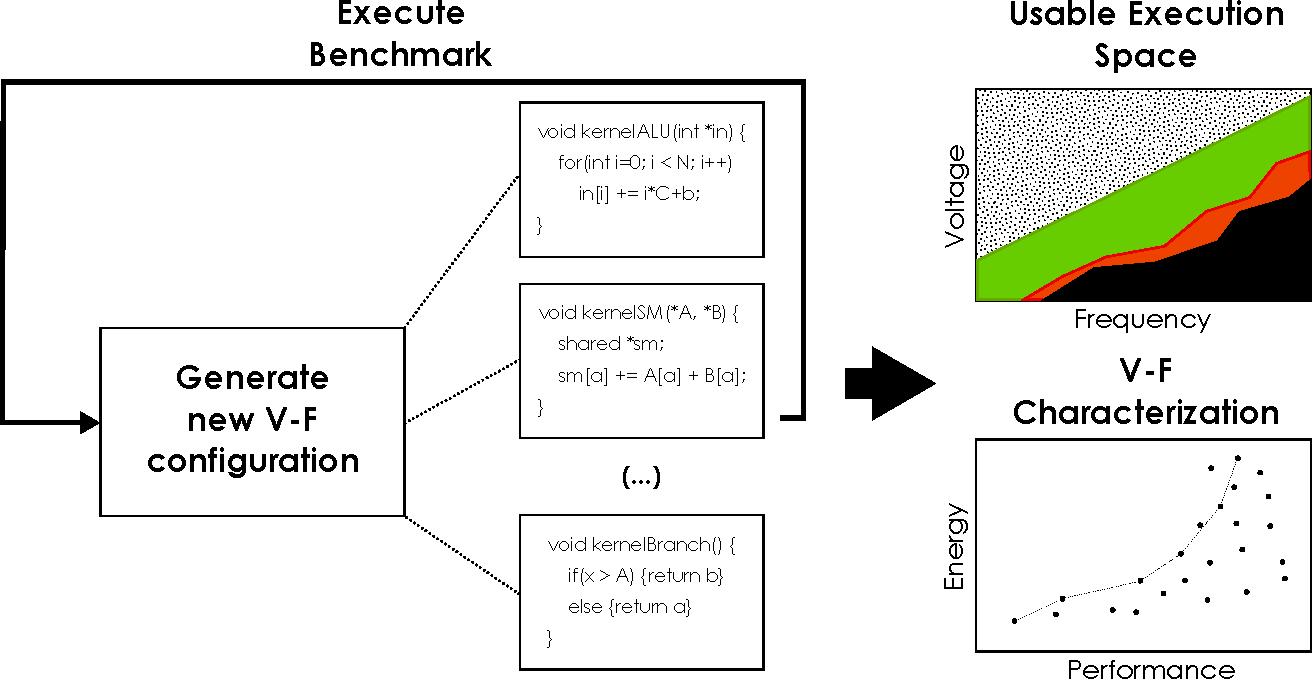
\includegraphics[width=0.8\textwidth]{Figures/GPU_characterization/gpu_char.pdf}
  \caption{.}
  \label{fig:gpu_char}
\end{figure}

Since the delay of a \acrshort{cmos} circuit is inversely proportional to the supply voltage $V_{DD}$ (and so, \acrshort{edp} is directly proportional to $V_{DD}$), computing the \acrshort{edp} brings the additional benefit of directly analyzing the effect of voltage change in the energy efficiency of the device.


\section{Characterization Benchmarks}
\label{sec:char_meth}

The devised set of benchmarks,  presented in Table~\ref{tab:benchmarks} and available as open-source\footnote{https://github.com/TheEmbbededCoder/GPU-Characterization}, individually characterize the different components of the \acrshort{gpu} architecture when subjected to the two \acrshort{dvfs} domains: \textit{core} and \textit{global memory}. The tested architectural components are \acrshort{dram}, Shared Memory, Cache L2 and \acrshort{alu}. In more detail, the \acrshort{dram} experiment covers the reading and writing operations, and the prolonged effects of undervoltage on memory retention, while the \acrshort{alu} tests include the Multiply and Accumulate (MAC) and non-linear operations, as well as the impact of branches. Overall, the developed benchmarks were crafted not only with the intention of stressing the individual components but doing so in a way that helps to answer the questions presented at the beginning of this chapter. Additionally, a coarser and more representative kernel that stresses multiple architecture elements in many \acrshort{gpgpu} applications - the reduction - is also evaluated.


\begin{table}[htb]
    \caption{Devised set of kernels to characterize GPU to Non-Conventional DVFS}
    \vspace{-5pt}
    \begin{center}
        \resizebox{\textwidth}{!}{%
        \begin{tabular}{lll}
            \hline
            \textbf{Micro-kernels}        & \textbf{Data Type} & \textbf{Objective} \\ \hline
            DRAM                                    & FP32, INT32                     & Minimum Read \& Write voltage, bit-flip, data-corruption                     \\[0.2em]
            &  & Effect of memory to compute bounded kernel on Core DVFS                     \\[0.5em]
            Cache L2                                & INT32                           & Minimum Read \& Write voltage, data-corruption                   \\[0.5em]
            Shared Memory                           & INT32                           & Minimum Read \& Write voltage, data-corruption                    \\[0.5em]
            ALU                                     & FP64/32/16, INT64/32/16/8       & Computation errors due to timing violations                   \\[0.5em]
            SFU                                     & FP64/32/16                      & Computation errors due to timing violations                   \\[0.5em]
            Branch                                  &                                 & Minimum voltage for correct schedualing operation                   \\[0.5em] %\hline
            %\textbf{App. kernels}   & \textbf{Data Type}              & \textbf{Objective} \\ \hline
            Mix (reduction)                               & FP64/32/16                      & Evaluates the simultaneous impact of stressing multiple GPU components                   \\\hline
        \end{tabular}%
        }
    \end{center}
    \label{tab:benchmarks}
\end{table}

On the listed benchmarks, the placeholder \texttt{DATA\_TYPE} is used to represent the different tested data types. The keyword is, following Table~\ref{tab:benchmarks}, equivalent to a standard integer and half, single and double precision data types depending on the benchmark. 
The objective is to assess the effect of changing the type of operands and computation precision on the critical path.

To guarantee that no compiler optimizations are performed on the tested variables, the keyword \texttt{volatile} is used.


\subsubsection{DRAM}

The benchmark on Listing~\ref{lst:DRAMbench} was designed (and validated through \acrshort{gpu} counters) to determine the impact of V-F scaling on a user-controlled memory to compute bounded kernel on both \acrshort{gpu} \acrshort{dvfs} domains. 

In the presented kernel, each thread is responsible for accessing the global memory and retrieving two values. The accesses are sequential between threads to guarantee maximum memory throughput and no accessing hazards
% (such as coalescing)
. These two values are summed and placed on an output vector. The constant $C$ determines the distance between accesses, and its value is sufficiently large to guarantee that the new data to be fetched is not present on the local caches.
For each data fetch, the defined \texttt{OPS} value controls the number of arithmetic operations to be performed before the data is written back on the \acrshort{dram}. A lower \texttt{OPS} value decreases the time between memory access, resulting in a more memory intensive kernel, that depending on the global memory, can become memory-bounded. On the other side, a higher \texttt{OPS} value results in the memory access to be more spaced in time, leading to a less memory intensive kernel and, eventually, even a compute bounded kernel.

The \acrshort{dram} \acrshort{dvfs} domain is responsible for controlling the voltage and frequency of the global \acrshort{gpu} memory. This \acrshort{dvfs} domain affects the memory throughput both on the reading and writing operations. With the characterization of this \acrshort{dvfs} domain, it is possible to judge the height of the global memory on the overall power and energy consumption and the impact of \acrshort{dram} performance when executing a more memory-bounded kernel. On the other hand, by assessing \acrshort{gpu} performance and energy consumption, with the same kernel, while acting on the core \acrshort{dvfs} domain, it concedes an understanding of how to best tune the core when the performance bottleneck is not within it.

\begin{figure}[h]
\begin{lstlisting}[language=C, caption=DRAM Benchmark Code, label=lst:DRAMbench, basicstyle=\footnotesize\ttfamily,abovecaptionskip=0pt, captionpos=b]
void  DRAMcode(DATA_TYPE *IN0, DATA_TYPE *IN1, DATA_TYPE *OUT) {
    const int ite = (blockIdx.x * THREADS + threadIdx.x) % MEM_BLOCK;
    volatile register DATA_TYPE r0;
    
    #pragma unroll
    for (int i = 0; i < N; i++) {
        r0= IN0[i * C + ite] + IN1[i * C + ite];
        #pragma unroll
        for(int j = 0; j < OPS; j++)  
            r0 += r0 * r0;
        OUT[threadId] = r0;
    }
}
\end{lstlisting}
\end{figure}

Listing~\ref{lst:DRAMbitflip} renders a benchmark designed to evaluate the occurrence of the phenomenon called \textit{bit-flip} and the preservation of the data in memory when exposed to undervoltage. A \textit{bit-flip} is an unintentional state switch from 0 to 1, or vice versa, of a bit stored on a \acrshort{dram} or other kinds of volatile memories. The phenomenon is usually addressed on space exploration devices. However, the work of Kim~\cite{kim_flipping_2014} exposed the existence of \textit{bit-flipping} on \acrshort{cpu} \acrshort{dram}, induced by the continuous activation of a \acrshort{dram} row that corrupts the data in near-by rows. The work was of such significant importance that the benchmark called \textit{rowhammer}\footnote{https://github.com/google/rowhammer-test} to test this exact problem started to be of severe importance to guarantee data integraty in novel systems. The benchmark on Listing~\ref{lst:DRAMbitflip} is a GPU implementation of \textit{rowhammer} that is going to be used to assess if undervolting the GPU can increase the possibility of such problem.

\begin{figure}[h]
\begin{lstlisting}[language=C, caption=DRAM Bit-Flip Stress Test Code - \textit{rowhammer} inspired  benchmark, label=lst:DRAMbitflip, basicstyle=\footnotesize\ttfamily,abovecaptionskip=0pt, captionpos=b]
void  DRAMstresser(DATA_TYPE *IN, DATA_TYPE *OUT) {
    const int ite = threadIdx.x;
    volatile register DATA_TYPE r0;
    
    // Initiate output memory
    OUT[ite] = IN[ite];
    OUT[ite + THREADS * BLOCKS] = IN[ite + THREADS * BLOCKS];
    
    for (int i = 0; i < N; i++) {
        r0 = IN[ite];
        #pragma unroll
        for(int j = 0; j < OPS; j++)  
            r0 += r0;
            OUT[ite] = r0;
    }
}
\end{lstlisting}
\end{figure}


\subsubsection{Cache}

As previously stated, even though the caches are part of the memory system, they are under the \textit{core} \acrshort{dvfs} domain. The devised benchmark presented on   Listing~\ref{lst:CacheL2bench}, follows a similar stressing pattern to Listing~\ref{lst:DRAMbench}. However, with the addition of the external \texttt{k} loop, the access pattern is repeated, and so, after the first execution, the data will be available on one of the two levels of cache. This kernel is then able to test (results verified with \acrshort{gpu} counters) both the state machine responsible for establishing the communicating between the cache and the \acrshort{dram} and the cache itself.

For the Cache benchmark, the number of issued requests to the cache and the DRAM-cache controller stays the same independently of the \texttt{OPS} value. However, the frequency of those requests is inversely proportional to \texttt{OPS}.

\begin{figure}[h]
\begin{lstlisting}[language=C, caption=CacheL2 Benchmark Code, label=lst:CacheL2bench, basicstyle=\footnotesize\ttfamily,abovecaptionskip=0pt, captionpos=b]
void  CacheL2code(DATA_TYPE *IN, *OUT) {
    const int ite = blockIdx * THREADS + threadIdx;
    volatile DATA_TYPE r0;
    
    for (k=0; k<N; k++) 
        #pragma unroll
        for(j=0; j<COMP_ITE; j++) {
            r0= IN[ite];
            #pragma unroll
            for(m=0; m<OPS; m++)    
                r0 += r0;
            OUT[ite] = r0;
        }
}
\end{lstlisting}
\end{figure}

\subsubsection{Shared Memory}

The benchmark that tests the Shared Memory is presented on the Listing~\ref{lst:SMcode}. This component is shared between threads in the same \acrshort{cu}/\acrshort{sm} and is used to perform communication between the different threads. As so, the developed benchmark performs uses the component to move data around. Similarly to the \acrshort{dram} and cache kernels, the variable \texttt{OPS} controls the time distance between memory requests, allowing for testing on the Shared Memory behaves with more or less stress on it. To guarantee correct and repeatable operations, the synchronization directive \texttt{\_\_syncthreads()} is used to synchronize all the threads that use the same shared memory.

\begin{figure}[h]
\begin{lstlisting}[language=C, caption=Shared Memory Benchmark code, label=lst:SMcode, basicstyle=\footnotesize\ttfamily, abovecaptionskip=0pt, captionpos=b]
void  SharedMemorycode(DATA_TYPE *IN, DATA_TYPE *OUT) {
    __shared__ DATA_TYPE shared[THREADS];
    const int ite = blockIdx * THREADS + threadIdx;
    
    int t = threadIdx.x;
    int tr = THREADS - t - 1;
    
    volatile register DATA_TYPE r0 = IN[ite];
    
    
    for (int i = 0; i < N; i += UNROLL_ITE) {
        #pragma unroll
        for(int j = 0; j < UNROLL_ITE; j++)  
            shared[t] = r0;
            __syncthreads();
            for(int k = 0; k < OPS; k++) 
                r0 += r0;
            r0 = shared[tr];
            __syncthreads();
    }
    
    OUT[ite] = r0;
}
\end{lstlisting}
\end{figure}

\subsubsection{MAC}

The arithmetic and logic unit (\acrshort{alu}) is responsible for performing all the \acrshort{gpu} computations.  As a component that performs such a different number of operations, a set of benchmarks was devised to stress this component in different ways. Overall, the focus of testing this component is to understand the degree of computational errors that may occur when overly undervoltage is applied, these resulting from timing violations across the critical path. Of significant importance when investigating the timing faults on the critical path is to test the influence of dependencies in the code, as these may influence how the warps scheduler orders the threads for execution on the \acrshort{cu}/\acrshort{sm}s. The benchmarks that test the \acrshort{alu} were designed to use all the available threads on the \acrshort{gpu}.

In Listing~\ref{lst:MACbench}, a greater emphasis was devoted to the \acrshort{mac} operation due to its prevalence in the Deep Learning (DL) domain. To test the influence of dependencies on the application, and so, the way the scheduler handles the execution of the different threads, a value between $0$ and $5$ is assigned to the variable \texttt{d} . When $d=0$, no dependencies exist in the code. The setup with $d=1$ represents the worst-case scenario, since introduces Read-after-Write (RaW) dependencies between all operations. This particular dependency setup was emphasized in the presented study, due to the variability of kernels executed by DL workloads. On the other hand, the setup with $d=3$ was considered a general case, where some dependencies still exist in the code, but the scheduler can mask some of them



\begin{figure}[htpb]
    \begin{lstlisting}[language=C, caption=MAC Benchmark Code, label=lst:MACbench, basicstyle=\footnotesize\ttfamily, abovecaptionskip=0pt, captionpos=b]
    void  MACcode(DATA_TYPE *IN, DATA_TYPE *OUT) {
        const int ite = (blockIdx * THREADS + threadIdx) * 4;
        
        volatile DATA_TYPE r0, r1, r2, r3, r4, r5;
        
        r0=IN[ite];  r1=IN[ite+1];  r2=IN[ite+2]; 
        r3=IN[ite+3];  r4=IN[ite];  r5=IN[ite+1];
        
        for(j=0; j<COMP_ITE; j++) {
            r0 += r0 * r{0-d}; r1 += r1 * r{1-d}; 
            r2 += r2 * r{2-d}; r3 += r3 * r{3-d}; 
            r4 += r4 * r{4-d}; r5 += r5 * r{5-d};
        }
        OUT[ite/4] = r0;
    }
    \end{lstlisting}
\end{figure}


\subsubsection{SFU - Non-Linear Operations}
    
Additional to the \acrshort{mac} operation, the \acrshort{alu} also needs to compute non-linear functions like exponential, logarithmic and trigonometric operations. For that it uses the special function unit (\acrshort{sfu}). Listing~\ref{lst:NonLinearbench} tests those operations to find if, when in use, they alter the critical path and so, negatively influence the guardband size.
    
\begin{figure}[htpb]
    \begin{lstlisting}[language=C, caption=Non-linear Operations Benchmark Code, label=lst:NonLinearbench, basicstyle=\footnotesize\ttfamily, abovecaptionskip=0pt, captionpos=b]
    void  NonLinearcode(DATA_TYPE *IN, DATA_TYPE *OUT) {
        const int ite = (blockIdx * THREADS + threadIdx) * 4;
        
        volatile DATA_TYPE r0, r1, r2, r3;
        
        r0=IN[ite];   r1=IN[ite+1];  
        r2=IN[ite+2]; r3=IN[ite+3];  
        
        for(j=0; j < N; j+= UNROLL_ITE) {
            #pragma_unroll
            for(j=0; j < UNROLL_ITE; j++) {
                r0 = exp(r2);   r1 = cos(r3);
                r2 = log(r0);   r3 = sin(r1);
            }
        }
        OUT[ite/4] = r0;
    }
    \end{lstlisting}
\end{figure}

\subsubsection{Branches}

Listing~\ref{lst:Branchesbench} renders a benchmark that tests the influence of the number of branches on a kernel. \acrshort{simt} processors do not favor the existence of branches on code, since it prevents the simultaneous execution of all threads. 
The scheduler's job is to organize the running threads in wavefronts to be simultaneously executed depending on the execution path dictated by the branches on the kernel. An increased number of branches makes the job of the scheduler more difficult. So, the developed benchmark analyses the influence of reducing the voltage on the scheduler operation. On Listing~\ref{lst:Branchesbench}, the \texttt{\#define BRANCHES} sets the desired number of branches to test between 1, 2, 4 and 8.

\begin{figure}[h]
\begin{lstlisting}[language=C, caption=Branches Benchmark Code, label=lst:Branchesbench, basicstyle=\footnotesize\ttfamily,abovecaptionskip=0pt, captionpos=b]
#define BRANCHES VALUE
void  Branchescode(DATA_TYPE *IN, *OUT) {
    const int ite = (blockIdx * THREADS + threadIdx;= % MEM_BLOCK;
    const int branch =  ite % BRANCHES;
    
    volatile register DATA_TYPE r0, r1, r2, r3;
    
    for (int i = 0; i < N; i++) {
        if(branch == 0)   r0 = IN[ite];
        #if BRANCHES >= 4
            else if(branch == 1)   r1 = IN[ite];
            else if(branch == 2)   r2 = IN[ite];
        #elif BRANCHES == 8
            else if(branch == 3)   r3 = IN[ite];
            else if(branch == 4)   r0 = IN[ite];
            else if(branch == 5)   r1 = IN[ite];
            else if(branch == 6)   r2 = IN[ite];
        #elif BRANCHES >= 2
            else {r3 = IN[ite];}
        #endif
        OUT[ite] = r0;
    }
}
\end{lstlisting}
\end{figure}

\subsubsection{Reduction}

The \texttt{reduction} benchmark listed in Listing~\ref{lst:Redbench} performs the reduction of a $N$-sized vector to $N/blockDim$, by performing an element-wise sum. The tested implementation of this operation is considered the one that achieves the highest performance, and so, it is the most widely used. It makes use of the shared memory to enable inter-thread communication and improve performance. Hence, this benchmark stresses all elements of the architecture (DRAM, Cache, shared memory and ALU) and allows to assess a more complex use-case, where a single kernel stresses multiple architectural units.

This kernel's objective is to test if the used component contribution can indicate the observed overall behavior of the kernel, or if there are higher-order interdependencies between the stressed units.

\begin{figure}[htb]
\begin{lstlisting}[language=C, caption=Reduction Kernel Code, label=lst:Redbench, basicstyle=\footnotesize\ttfamily,abovecaptionskip=0pt, captionpos=b]
void Reduction(DATA_TYPE * idata, DATA_TYPE * odata){
    __shared__ DATA_TYPE s[THREADS];
    unsigned int i, k, t = threadIdx;
    unsigned int index = blockIdx * blockDim * N + threadIdx;
    
    // cooperative load from global to shared memory
    s[t] = 0;
    for (i=0; i< 4; i++, index += blockDim.x)
        s[t] += idata[index];
    __syncthreads();
    
    // do reduction in shared memory
    if(t < 64) {
        s[t] += s[t+64]; 
        __syncthreads(); 
    }
    
    if(tid <32){
        s[t] += s[t+32];   s[t] += s[t+16];
        s[t] += s[t+8];    s[t] += s[t+4];
        s[t] += s[t+2];    s[t] += s[t+1];
    }
    
    // write result for this block to global mem
    if(t == 0) odata[blockIdx.x] = s[0];
}
\end{lstlisting}
\end{figure}


%%%%%%%%%%%%%%%%%%%%%%%%%%%%%%%%%%%%%%%%%%%%%%%%%%%%%%%%%%%%%%%%%%%%%%%%
\section{Experimental Setup}

The devised benchmarks were applied to characterize an AMD Vega 10 Frontier Edition \acrshort{gpu}, whose specifications are presented in Table II~\ref{tab:Vega10specs}. 

\begin{table}[htbp]
    \caption{AMD Vega 10 Frontier Edition Specifications.}
    \begin{center}
        % \resizebox{0.48\textwidth}{!}{%
            \begin{tabular}{lr}
                \hline
                {Architecture} & GNC5\\
                {CUs} & 64\\
                {DRAM size} & 16 GB\\
                {Core frequency range [MHz]} & [852 - 1980]\\
                {Core voltage range [mV]} & [900 - 1200]\\
                {DRAM  frequency range [MHz]} & [500 - 1200] \\ 
                {DRAM  voltage range [mV]} & [800 - 1200] \\
                \hline
                \multicolumn{2}{c}{\textbf{Default Frequency-Voltage (F-V) setups}}\\
                \hline
                {\textit{Core} F-V [MHz ; mV]} & [995;900, 1140;950, 1350;1050, \\
                \multicolumn{2}{r}{ 1440;1100, 1530;1150, 1600;1200{]}} \\
                {\textit{DRAM} F-V [MHz ; mV]} & [500;900, 800;950, 950;1000] \\
                \hline
            \end{tabular}%
        % }
    \end{center}
    \label{tab:Vega10specs}
\end{table}

By default, the GPU driver establishes the two sets of Frequency-Voltage (F-V) setups presented in Table~\ref{tab:gpulevels}. However, the \acrshort{gpu} vendor rocm-smi\footnote{github.com/RadeonOpenCompute/ROC-smi} tool allows for independent control over frequency and voltage. The following section presents the capabilities of the software tool and Annex A shows a more comprehensive description and user manual of rocm-smi. Finally, to allow a greater evaluation range, the GPU power cap was changed from the default 220W to 300W (matching the GPU thermal design). This GPU was installed on a machine equipped with an Intel i7 4770K CPU, with 32 GB of main memory. 




\subsection{Voltage and Frequency control API}
The ROCm System Management Interface (rocm-smi) \cite{noauthor_radeonopencompute/roc-smi_2019} is a user-friendly command-line application for manipulating the Radeon Open Compute Kernel (ROCk). Using it makes it possible to know and control the state of the GPU devices present in the system. 

\begin{itemize}
\item \textbf{GPU utilization:} Retrieves the current utilization rates corresponding to the device's major subsystems, one value for the processing core and other for the main device memory. The rate is computed over a specific time interval set on the device driver. The processing core utilization reflects the percentage of time that the GPU core is being used to perform computations. In contrast, the main device memory utilization reflects the percentage of time the memory was being read or written.

\item \textbf{GPU power}: Retrieves the average power used by the device. Similarly to the utilization rate, the average power is computed over a defined time interval, during which a number of power samples are taken.

\item \textbf{Clock rate and voltage level:} Retrieves both the clock frequency and device voltage level. Of significant importance is that the voltage retrieved corresponds to the maximum measured value between the \acrshort{gpu} core and the main device memory voltage. Current versions of AMD \acrshort{gpu}s do not allow for querying the specific voltage value of the different \acrshort{dvfs} domains.

The tool also displays two tables: the first, showing the eight pairs of clock frequency/voltage level of the GPU core and the second, showing four pairs of the same parameters related to the device memory. These two tables correspond to the 8 and 4 performance levels that the device kernel can apply to the GPU core and memory, correspondingly.
\end{itemize}

The rocm-smi interface also allows querying the device temperature, the current fan speed, and the selected performance level.

rocm-smi also provides a mechanism to control and change some of the device parameters:
\begin{itemize}
\item \textbf{Set performance level:} Allows the user to select the desired performance level of the GPU core and device memory, disabling the driver's automatic performance level management system.
\item \textbf{Set clock rate and voltage level:} Set the clock frequency and the voltage level of any of the performance levels of both the GPU core and memory. 
\item \textbf{Reset clock rate and voltage level:} Resets the clock rates and voltage level to the default values.
\end{itemize}

Additionally, the interface allows the user to manually set the fan speed required to guarantee the same temperature level for all executed tests.

The versatility and ability to independently control the clock rate and voltage level of the device, enabled by rocm-smi, was the defining factor for choosing an AMD GPU over the more popular NVIDIA options.


\subsection{Testing procedure}
\label{sec:ex_setup}

The default frequencies of the GPU \textit{Core} and \textit{DRAM} domains, presented in Table~\ref{tab:Vega10specs}, were selected as the starting point for the non-conventional DVFS. For each frequency, the devised experiment started at the maximum voltage ($1200mV$) and a gradual undervoltage of the GPU V-F domain under test was applied with $50mV$ steps. For each step, the benchmarks were executed ten times to obtain the median value of the execution time and energy consumption. 

All the tests were performed using randomly generated inputs to avoid any bias incurred by the considered data values. Integer values were obtained from a normal distribution across their complete 32-bits range, while floating-point operands were generated using a uniform distribution in the interval $[0.1~;~1]$. The choice for limiting floating-point range to an interval with a maximum value inferior to one ensures that operations are never applied to numbers with a significantly different exponent value, thus avoiding rounding errors that would conduct to the discard of the operator with the lowest absolute value.

While performing the undervoltage, the GPU goes through three distinct stages. At the first stage (\textit{working}), the \ac{gpu} works regularly, and no changes are detected in the application output. Then, by continuing the \ac{gpu} voltage reduction, some \textit{computational errors} are introduced and some application outputs change when compared with the default voltage setup. For integer experimentation, a computational error is considered if the output value differs from the default run, for the floating-point operation, the relative error between the default and non-conventional run is computed for each individual result. When the relative difference between the above is bigger than $10^{-4}$, it is said that the result has \textit{computational errors}.
By reducing the GPU voltage beyond this stage, the \ac{gpu} enters into the \textit{crash} state, becoming unusable.

To accurately determine the areas of interest (i.e., when infrequent computation errors occur) and to determine the crash point, the undervoltage step was reduced to $10mV$. Furthermore, when dealing with the \acrshort{DRAM} V-F domain, the \textit{Core} V-F domain was set to default values; for the \textit{Core} V-F domain, the highest frequency and default voltage of the \textit{DRAM} was selected. The GPU power consumption was measured using gpowerSAMPLER\footnote{github.com/hpc-ulisboa/gpowerSAMPLER}~\cite{guerreiro_gpgpu_2018}, at every millisecond. At the end of the execution, the energy is computed as the integral of all the measurements taken. 

%%%%%%%%%%%%%%%%%%%%%%%%%%%%%%%%%%%%%%%%%%%%%%%%%%%%%%%%%%%%%%%%%%%%%%%%
\section{Limiting components to the voltage exploration space}
\label{sec:limiting_components}

The execution of the different benchmarks while controlling the V-F values allowed us to study how much voltage guardband each component has. More specifically, to explore and quantify how far it is possible to decrease the operating voltage from each default frequency level while measuring the impact on the application output and working capabilities of the \acrshort{gpu} device. 


\subsection{DRAM}

Figure~\ref{fig:DRAM_guardband} illustrates the usable voltage range of the DRAM domain. Across the complete, tested frequency range, it is possible to undervolt the memory to $800mV$, independently of the value of \texttt{OPS} (parameter variation between 0 and 50 operations, see Listings~\ref{lst:DRAMbench}).
The conducted experiment shows that no computation error or crashes happen for the default frequencies within the complete voltage range. The kernel runs successfully, with no perceptible change in the output.


\begin{figure}[htb]
  \centering
  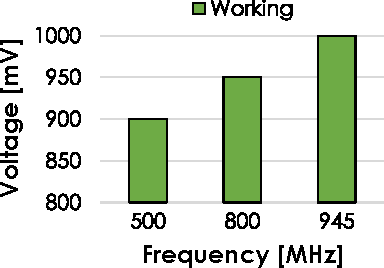
\includegraphics[width=0.35\textwidth]{Figures/GPU_characterization/DRAM_Guardband.pdf}
  \caption{DRAM domain - Usable DRAM voltage for each frequency configuration.}
  \label{fig:DRAM_guardband}
\end{figure}

The result and strong conclusion derived from the previous experience was further verified with the use of the kernel of Listing~\ref{lst:DRAMbitflip}. It is of extreme importance to validate if the use of lower voltage values induces data corruption on two edge cases: extreme use of part of \acrshort{dram} and prolonged data storage. That said, the kernel was executed, and after periods of 1, 2, 5, 10, 30 minutes and 1, 2, 4 and 8 hours, the output data was retrieved and compared to the original set. Again, no perceptible change in the output was detected, further validating the previous result and assessing that the \acrshort{dram} can be successfully used with lower voltage levels. 

\subsection{Cache}

Fig.~\ref{fig:CacheL2_guardband} presents the usable voltage interval for different frequency setups. For frequencies below $1530$MHz, no computation errors or crashes were observed, with the \acrshort{gpu} correctly working at the lowest voltage across all the tested frequencies. Only for frequencies as high as $1530$ and $1600$ MHz performing undervoltage resulted in the program crashing. A critical observation is that no computation errors occur, meaning that this architectural component either works normally or makes the GPU immediately to crash. This phenomenon is of significant importance to determine the root cause of failures, since if it is observed \acrshort{gpu} crash without prior computation errors, this may be the preeminent component causing it.
Furthermore, an increase in \texttt{OPS} allows for a higher amount of undervolt. Since this change only affects the stress over the DRAM-Cache controller (the number of cache accesses and hit-rate maintains the same), it can be concluded that it is the Cache-DRAM controller that limits the undervoltage range and not the memory elements of the cache.


\begin{figure}[htb]
  \centering
  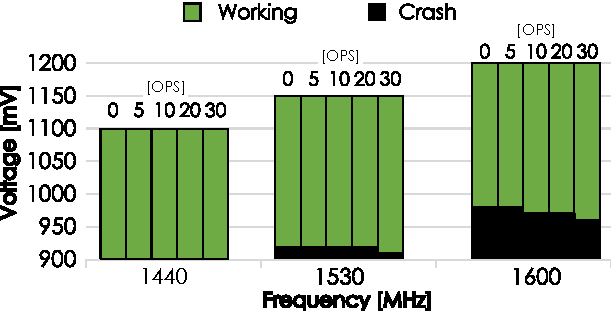
\includegraphics[width=0.5\textwidth]{Figures/GPU_characterization/CacheL2_guardband.pdf}
  \caption{Core domain - Usable CacheL2 voltage for each frequency configuration with varying cache stress ($OPS$ value).}
  \label{fig:CacheL2_guardband}
\end{figure}


\subsection{Shared Memory}

\begin{figure}[htb]
  \centering
  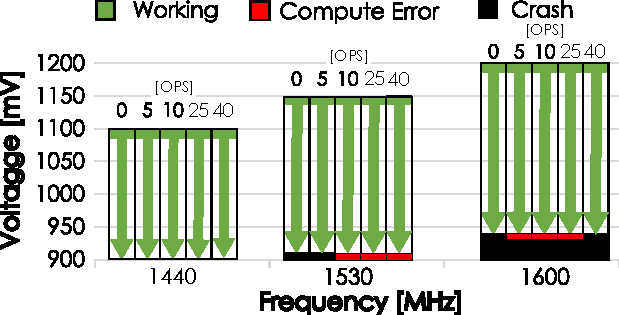
\includegraphics[width=0.5\textwidth]{Figures/GPU_characterization/SharedMemory_guardband.pdf}
  \caption{Core domain - Usable Shared voltage for each frequency configuration with varying shared memory stress ($OPS$ value).}
  \label{fig:CacheL2_guardband}
\end{figure}

\subsection{MAC}

Fig.~\ref{fig:MAC_guardband} represents the usable undervoltage range for the \acrshort{alu} benchmark. The presented benchmark was performed for integer and floating-point data types and with different float precision. In all tests, for frequencies below $1440$~MHz, the benchmark successfully runs for all voltage values. For higher frequencies, it is observed that after a certain amount of undervoltage, computation errors start appearing. The GPU crashes if a further undervoltage level is applied. 
It is also observable that the voltage margin increases with the operating frequency, from around $170$mV for $1440$MHz to around $210$mV for $1600$MHz (values for single-precision floating-point).

The dependencies effect varied from integer to floating-point operation. In the first case, the dependencies on the code do not affect the size of the voltage margin. In the second case, the existence of dependencies in the code reduces the size of the voltage margin. In general, when compared with the setup with no dependencies (\texttt{d=0}), the undervoltage range of the benchmark configuration that represent the general case (\texttt{d=3} - see Listings~\ref{lst:MACbench}) is reduced by $10$mV. 

\begin{figure}[htb]
  \centering
  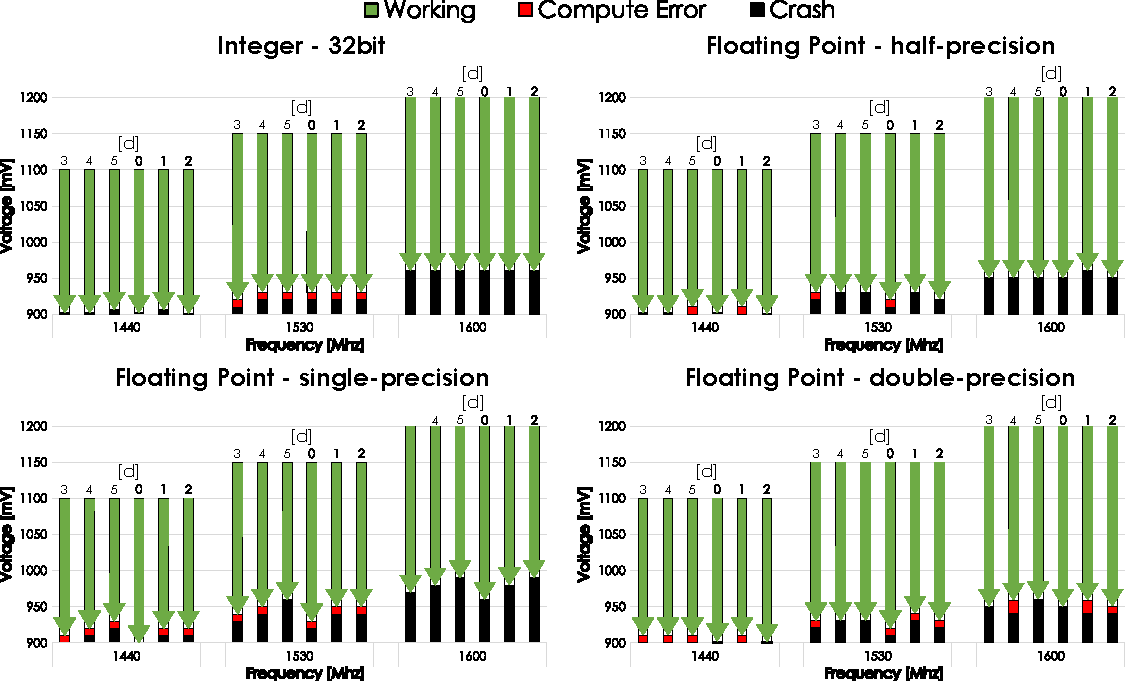
\includegraphics[width=1\textwidth]{Figures/GPU_characterization/MAC_Guardband.pdf}
  \caption{Core domain - Usable ALU-MAC voltage for the different data types and operand's precision.}
  \label{fig:MAC_guardband}
\end{figure}

\subsection{Non-linear Operations}

\begin{figure}[htb]
  \centering
  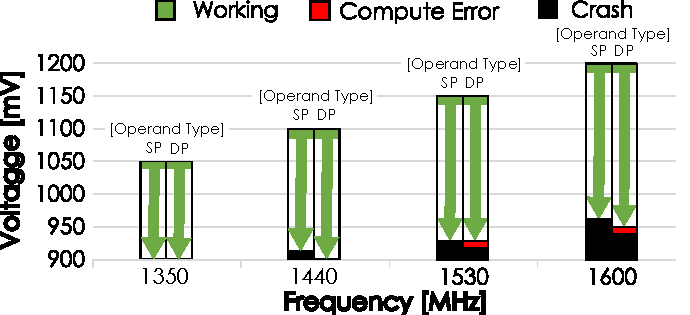
\includegraphics[width=0.6\textwidth]{Figures/GPU_characterization/SFU_guardband.pdf}
  \caption{Core domain - Usable Special Function Unit voltage for each frequency configuration with varying operand type: SP - Single Precision Floating-Point, DP - Double Precision Floating-Point.}
  \label{fig:SFU_guardband}
\end{figure}

\subsection{Branches}

\begin{figure}[htb]
  \centering
  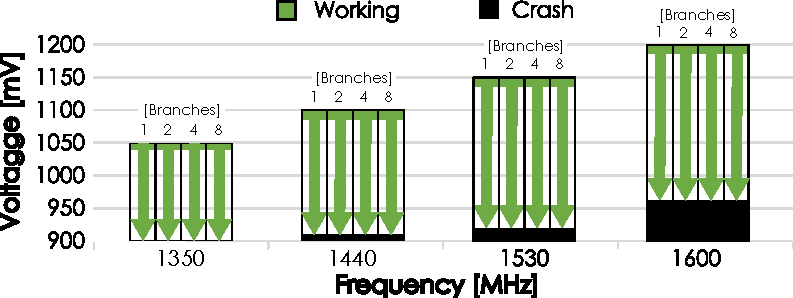
\includegraphics[width=0.7\textwidth]{Figures/GPU_characterization/Branches_guardband.pdf}
  \caption{Core domain - Usable Branches voltage for each frequency configuration with varying number of branches per iteration.}
  \label{fig:Branches_guardband}
\end{figure}

\subsection{Reduction}

\begin{figure}[htb]
  \centering
  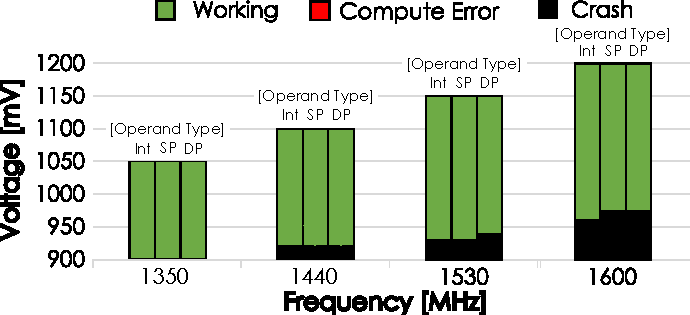
\includegraphics[width=0.6\textwidth]{Figures/GPU_characterization/Reduction_guardband.pdf}
  \caption{Core domain - Usable voltage for Reduction benchmark for each frequency configuration with varying operand type: Int - 32-bit Integer, SP - Single Precision Floating-Point, DP - Double Precision Floating-Point.}
  \label{fig:Reduction_guardband}
\end{figure}


\subsection{General Comments and Remarks}

\begin{figure}[h]
    \centering
        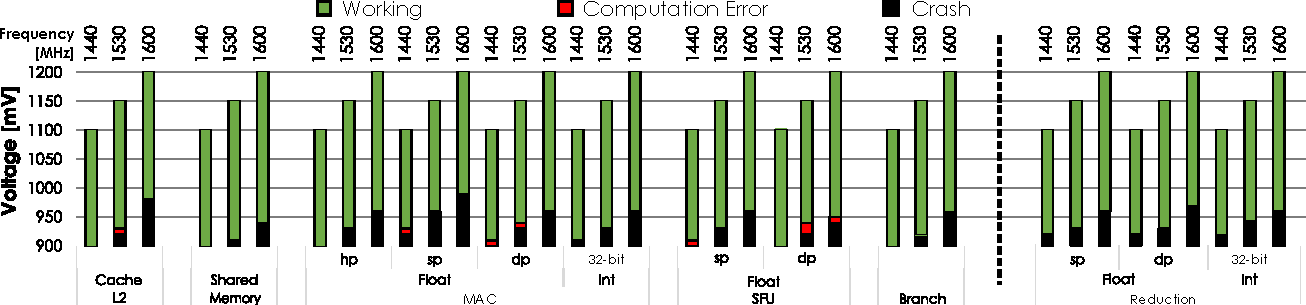
\includegraphics[width=1\textwidth]{Figures/GPU_characterization/Comparison_Guardband.pdf}
        \caption{Comparison of usable GPU core voltage ranges for all the considered architectural components of the GPU.}
    \label{fig:Guardband_comparison}
\end{figure}

%%%%%%%%%%%%%%%%%%%%%%%%%%%%%%%%%%%%%%%%%%%%%%%%%%%%%%%%%%%%%%%%%%%%%%%%
\section{V-F decoupled scaling GPU behaviour}
\label{sec:gpu_behaviour}

\subsection{DRAM}

\begin{figure}[htb]
  \centering
  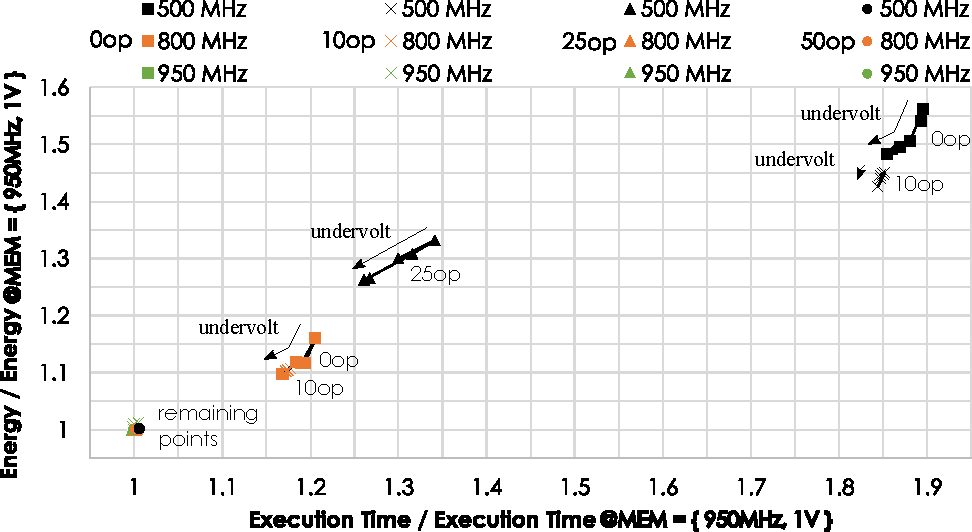
\includegraphics[width=0.8\textwidth]{Figures/GPU_characterization/DRAM_behaviour.pdf}
  \caption{DRAM domain - Normalized energy consumption and execution time.}
  \label{fig:DRAM_behaviour}
\end{figure}
\subsection{Cache}
\subsection{Shared Memory}
\subsection{MAC}
\subsection{Non-linear Operations}
\subsection{Branches}
\subsection{Reduction}
%%%%%%%%%%%%%%%%%%%%%%%%%%%%%%%%%%%%%%%%%%%%%%%%%%%%%%%%%%%%%%%%%%%%%%%%
\section{Summary}


\subsection{Memory V-F Domain}
\label{section:memory}



\subsection{Core V-F Domain}
\label{section:core} % file "Thesis_Implementation.tex"
\cleardoublepage

%%%%%%%%%%%%%%%%%%%%%%%%%%%%%%%%%%%%%%%%%%%%%%%%%%%%%%%%%%%%%%%%%%%%%%%%
%                                                                      %
%     File: Thesis_Results.tex                                         %
%     Tex Master: Thesis.tex                                           %
%                                                                      %
%     Author: Andre C. Marta                                           %
%     Last modified :  2 Jul 2015                                      %
%                                                                      %
%%%%%%%%%%%%%%%%%%%%%%%%%%%%%%%%%%%%%%%%%%%%%%%%%%%%%%%%%%%%%%%%%%%%%%%%

\chapter{Decoupled V-F Optimization Mechanism}
\label{chapter:mech}


The preliminary results that were presented in the previous chapter denote the idea that energy-efficiency (in particular, the \acrshort{edp} metric) of an out-of-the-shelf \acrshort{gpu} can be significantly improved if a specific non-conventional V-F pair is applied on the Core \acrshort{dvfs} domain. 

However, the preliminary experiments that were conducted in the previous chapter, did not include any adaptation of the frequency and voltage scaling in a dynamic way, being one of this dissertation's objectives.
To address this dynamic tunning of frequency and voltage, while using the increased exploration space of the operation conditions (and taking into account that it is necessary to guarantee a safe \acrshort{gpu} operation), two approaches are now envisioned: creating a forecasting model, or creating an online optimization mechanism.

The forecasting model would predict the most appropriate V-F pair based on the application executing code (static analysis of the Assembly code) and performance counters (run-time trace of the application being executed). This option would have the benefit of allowing the complete execution of the target application under the best possible configuration. However, such a forecasting model would also have to take into consideration the \acrshort{gpu} temperature, utilization (the target application being executed by itself or concurrently with others) and more importantly, it would be very tied to a specific \acrshort{gpu} model. Consequently, this option would become rather complex and not easily scalable between different \acrshort{gpu}s.

On the other hand, an online iterative optimization mechanism could target the native code repetition patterns usually observed in \acrshort{gpgpu} applications. For these applications, the best overall configuration is the best V-F pair for each algorithm's step, so by intelligently exploring a V-F configuration in each iteration of the user application, it is possible to find the best V-F pair for the running algorithm.
This approach brings the added advantage of optimizing not only the \acrshort{gpu} pre-execution state, accounting for the aging and all \acrshort{pvt} variations, but it also reacts to the on-execution state, changing the V-F configuration in accordance with device temperature and utilization.



Due to the added benefits of targeting the current \acrshort{gpu} state, the second approach, consisting on the creation of an online V-F optimization mechanism, was followed. 
Accordingly, this chapter is divided into three sections with the following outline: Section~\ref{section:opt} presents a description of the developed optimization mechanism; Section~\ref{sec:implementation} describes the interfaces and other programs that were used to develop the devised mechanism. Finally, Section~\ref{sec:usage} presents a description of the implemented functions and how they should be integrated in the user application.



%%%%%%%%%%%%%%%%%%%%%%%%%%%%%%%%%%%%%%%%%%%%%%%%%%%%%%%%%%%%%%%%%%%%%%%%
\section{Decoupled V-F Optimization Mechanism description}
\label{section:opt}


The envisioned V-F optimization mechanism aims to search and find the optimal V-F configuration to the running \acrshort{gpgpu} application and current \acrshort{gpu} state, optimizing it for \textit{performance}, \textit{energy consumption} or \textit{energy-efficiency} (\acrshort{edp}). As it was described in the previous chapter, this optimal V-F configuration depends on the type of computations being performed, the \acrshort{gpu} temperature, utilization, \acrshort{pvt} variations and aging, and it is obtained by searching over an exploration space based on the set of observations that were obtained from the set of experiments covered on chapter~\ref{chapter:gpu_char}. 

An essential consideration that must be taken into account when designing the optimization mechanism is the time that the regular \acrshort{gpu}s voltage-frequency controllers take to change these parameters. As described in Chapter 2, the controllers equipping out-of-the-shelf devices take between 200 to 500 ms to change and set the new V-F pair, making them unsuitable for continuously adapting to each operation executed on the device. Instead, it is necessary to group a collection of operations (as described, a complete iteration of the user application) and find the most suitable V-F configuration for that set.
In particular, it is necessary to allow a portion of time between the V-F changes in order to guarantee that the control mechanism has time to perform the change and stabilize both the frequency and the voltage before continuing to execute the computation.

As it was previously referred, at the time of this dissertation, only AMD provides the necessary tools to independently control voltage and frequency, being that a requirement that is out of our control when designing this tool. However, if other manufacturers develop command-line applications that provide the same degree of control, this optimization mechanism can easily be ported to accommodate the same.


\subsection{Architecture and Execution Overview}


The devised V-F optimization mechanism follows the block diagram of Figure~\ref{fig:opt_mech}, consisting of a two-phase process. In the first phase, data about the \acrshort{gpu} \acrshort{dvfs} system is gathered and application baseline metrics are taken. In the second phase, the user application algorithm is executed while searching for the best V-F pair. When the best V-F configuration is found, the devised optimization mechanism continues to monitor the user application to guarantee a safe operation, reacting to eventual \acrshort{gpu} state changes (for example, changing temperature).

\begin{figure}[htb]
  \centering
  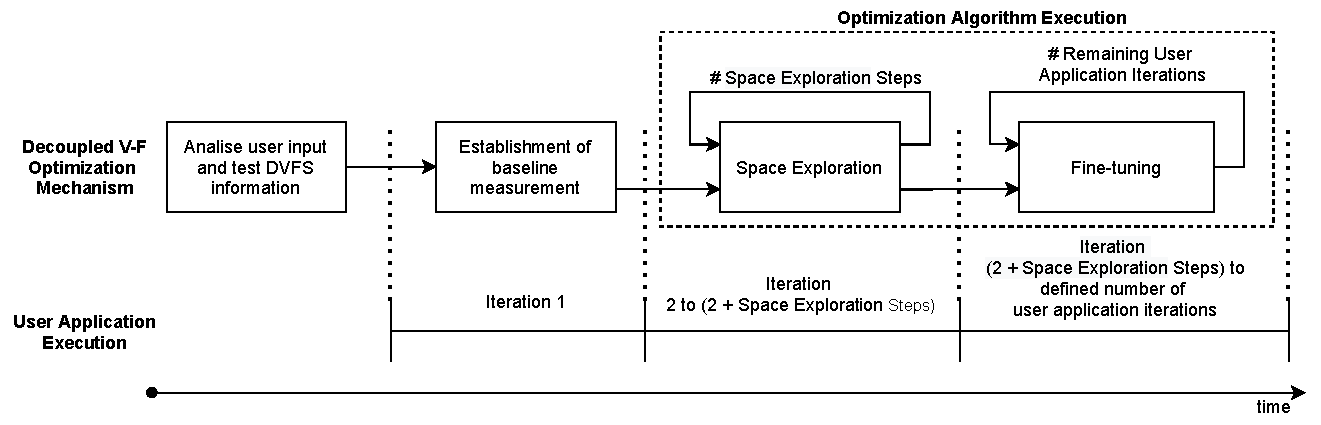
\includegraphics[width=\textwidth]{Figures/Optimization/full_mech6.pdf}
  \caption{V-F Optimization Mechanism Block Diagram.}
  \label{fig:opt_mech}
\end{figure}

On this context, and depending on the considered optimization metric, the best V-F configuration is the one that achieves the highest \textit{performance}, lowest \textit{energy consumption}, or higher \textit{energy efficiency} for the running application. Taking into account the main objective of this dissertation, the chosen and exemplified metric from now on is \textit{energy efficiency}, evaluated using the \acrshort{edp} metric, where 
\begin{equation}
	EDP=energy * computation \: time.
	\label{eq:edp}
\end{equation}

The following sections describe the operation of each stage of the devised optimization algorithm.

\subsubsection{Analysis of user input and test DVFS information}

The proposed procedure starts by receiving the user input that summarizes the characterization results obtained in Chapter 3. The summary includes the tested Core \acrshort{dvfs} frequencies and allowed voltage range for each frequency that guaranteed a correct operation in all tested benchmarks. Figure~\ref{fig:input} shows an example input to the mechanism and their corresponding usable execution space. There, the user should indicate the tested frequencies and corresponding $V_{max}$ and $V_{min}$. After that, information about the current \acrshort{gpu} device \acrshort{dvfs} system is gathered and compared to the user input, guaranteeing the validity of the proposed usable execution space, which will be explored by the optimization mechanism.


\begin{figure}[!htb]
    \begin{center}
        \begin{minipage}[t]{.5\textwidth}
            \vspace{0pt}
            \centering
            \resizebox{\textwidth}{!}{%
            \begin{tabular}{l}
                \texttt{[Frequencies] 990  1140  1270  1350  1440  1530  1600}\\
                \texttt{[Vmax]        900  950   1000  1050  1100  1150  1200}\\
                \texttt{[Vmin]        900  900   900   950   975   1000  1075}
            \end{tabular}
            }
        \end{minipage}%
        \begin{minipage}[t]{.45\textwidth}
            \vspace{0pt}
            \centering
            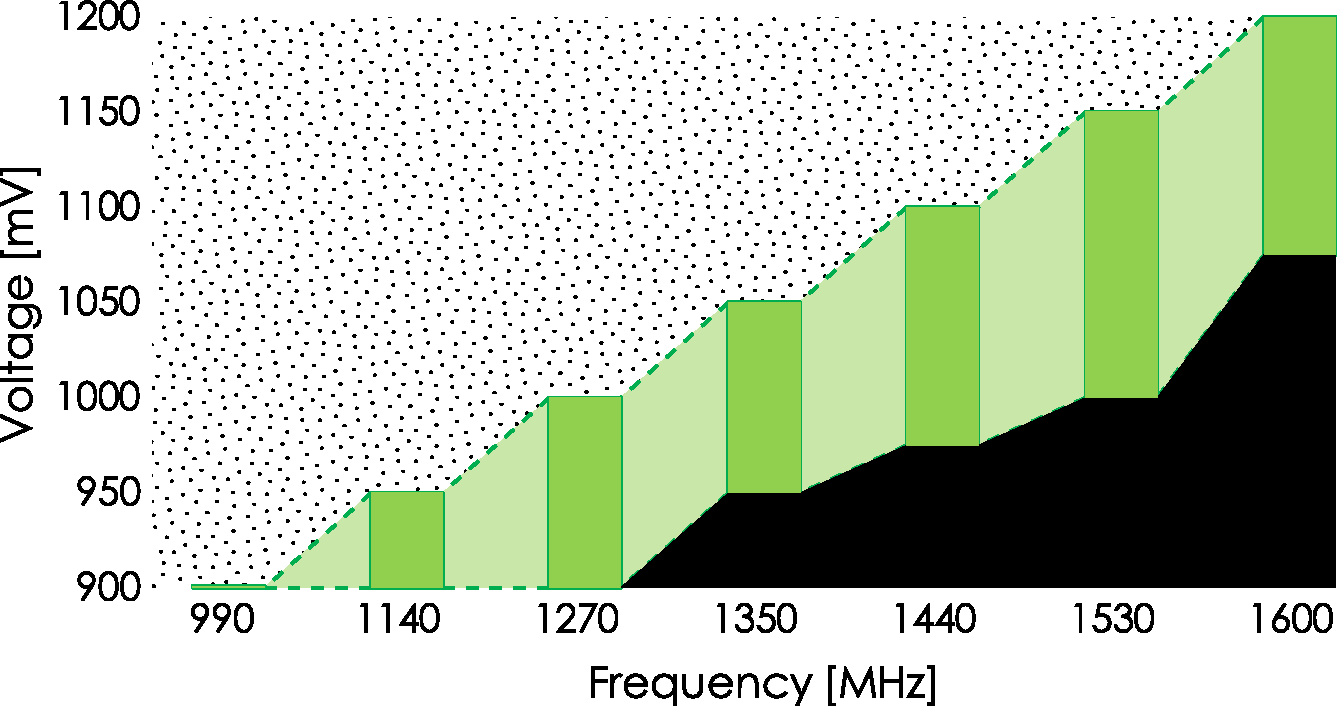
\includegraphics[width=\textwidth]{Figures/Optimization/UESex.pdf}
            \label{fig:uesex}
        \end{minipage}
    \end{center}
    \label{fig:input}
    \caption{Input example for the optimization mechanism (left) and correspondent usable execution space chart (rigth). Black-shaded regions represent unusable operation points (GPU crash), while green shaded regions represent tested DVFS operating points.}
\end{figure}





% \begin{figure}[!htb]
%     \centering
%     \begin{subfigmatrix}{2}
%     \subfigure[Data input.]{
%       \label{tab:input}
%       \resizebox{0.4\textwidth}{!}{%
%         \begin{tabular}{l}
%             \texttt{[Frequencies] 990  1140  1270  1350  1440  1530  1600}\\
%             \texttt{[Vmax]        900  950   1000  1050  1100  1150  1200}\\
%             \texttt{[Vmin]        900  900   900   950   975   1000  1075}
%         \end{tabular}
%         }
%     }
%       \subfigure[Example Usable Execution Space.]{
%         \centering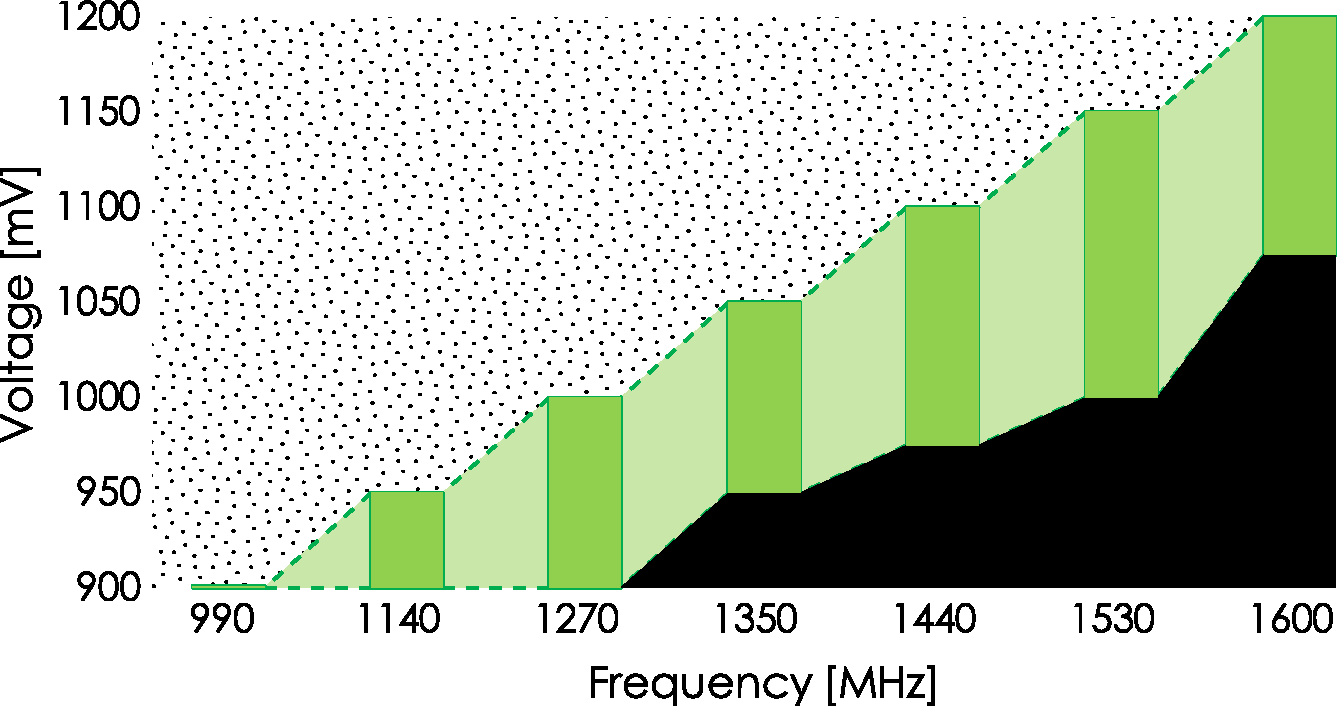
\includegraphics[width=0.45\textwidth]{Figures/Optimization/UESex.pdf}
%         \label{fig:uesex}
%       }
%     \end{subfigmatrix}
%     \caption{Input example for the optimization mechanism. - QUAL ESCOLHER???}
% \end{figure}



\subsubsection{Establishment of baseline measurement}

In this stage, a single step of the user application is executed with the highest frequency-voltage pair that was identified on the previous step, while the execution time and energy consumption are measured to compute the baseline \acrshort{edp} value. All the following measurements are normalized to this first result, in order to compare the results at different V-F configurations.

\subsubsection{Optimization Algorithm Execution}

In general, each stage of the Optimization Algorithm Execution phase (\textit{Space Exploration} and \textit{Fine-Tuning}) follows the flowchart presented in Figure~\ref{fig:flowchart}. This has three distinct steps, denoted as \textit{Application execution and metrics}, \textit{V-F control} and \textit{Online monitorization}. The first and last steps are the same for the two stages of the Optimization Algorithm Execution. However, the second \textit{V-F control} step, varies between the \textit{Space Exploration} and \textit{Fine-Tuning} stages, as depicted above.

\begin{figure}[h]
  \centering
  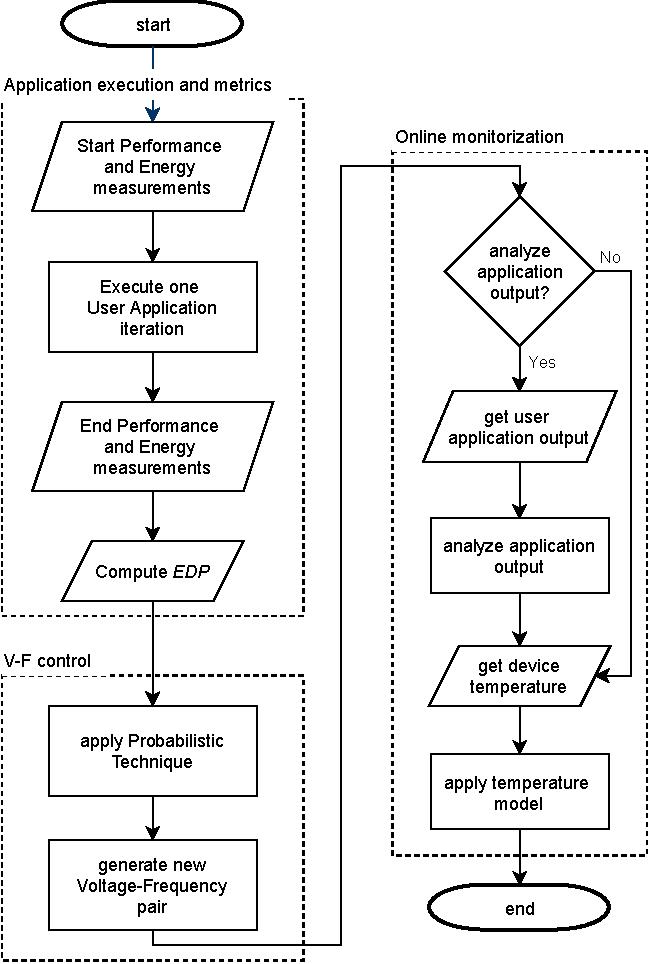
\includegraphics[height=0.95\textwidth]{Figures/Optimization/flowchart.pdf}
  \caption{Flowchart of each iteration of the Optimization Algorithm Execution.}
  \label{fig:flowchart}
\end{figure}

The following subsections describe the operation of each step of the optimization algorithm execution stage.

\bigskip
\noindent\underline{Application execution and metrics}
\bigskip

On the \textit{Application execution and metrics} step, an iteration of the user application is executed, and the performance and energy consumption is evaluated to compute the optimization metric \acrshort{edp}. 

\bigskip
\noindent\underline{V-F control}
\bigskip


This step aims to analyze the considered optimization metric, \acrshort{edp} value, and, according to a probabilistic technique, accept or reject the tested V-F configuration to generate a new V-F pair.

As previously stated, the devised V-F Optimization Mechanism works by iteratively exploring the usable execution space V-F configurations, while measuring the resulting \acrshort{edp} value for each of them. Hence, the challenge here is to find the most suitable configuration (corresponding to the V-F pair that minimizes the target metric) without testing every possible configuration, as performed on Chapter~\ref{chapter:gpu_char}. A panoply of algorithms could be employed to decide which configurations to test, while searching for the global minimum of the $EDP(f, V)$ function. 
The selection of such probabilistic technique considered the use of the mathematical optimization technique of Hill Climbing~\cite{vaughan_simultaneous_2005} or the metaheuristic algorithm of Simulated Annealing~\cite{kirkpatrick_optimization_1983} (depending on the Optimization Algorithm Execution stage), supported on the first by improving its ability to escape local minimums, and so improving the chances of finding an approximate global optimum in a fixed amount of iterations. 

In more detail, if the achieved \acrshort{edp} value is smaller than the current baseline after the \textit{Application execution and metrics} stage, the current V-F configuration is stored alongside the corresponding \acrshort{edp} value as the current \textit{V-F pair baseline} and it is inserted on a list of best configurations. Then, based on the current \textit{V-F pair baseline}, the new V-F configuration is randomly generated using the algorithms depicted ahead.


\bigskip
V-F control during Space Exploration stage
\bigskip

As the name implies, this step objective is to explore the usable execution space, finding a V-F configuration that achieves a good approximation of $min(EDP(f, V))$ in a reduced number of iterations.
To tackle this problem, the \textit{Simulated Annealing} algorithm was applied as the adopted Probabilistic Technique (see Figure~\ref{fig:flowchart}) of this stage. Since it is impossible to guarantee that $EDP(f, V)$ does not contain any local minimums (without any prior knowledge), it is preferable to use an algorithm that reduces the chance of those impacting the final chosen V-F configuration. In practice, this is reflected by the algorithm allowing for some tested V-F pairs that did not achieve the best \acrshort{edp} value, to be accepted and stored as \textit{V-F pair baseline} and so, escaping from a possible local minimum. Based on the current \textit{V-F pair baseline}, the new V-F configuration is randomly generated according to Algorithm~\ref{alg:space-frequency} followed by Algorithm~\ref{alg:space-voltage}.

\begin{algorithm}
    \caption{Space Exploration - Generate new frequency.}
    \label{alg:space-frequency}
 \hspace*{\algorithmicindent} \textbf{Input:} $baseline\_frequency$: current baseline frequency \\
 \hspace*{\algorithmicindent} \textbf{Input:} $default\_frequencies$: list of available default frequencies \\
 \hspace*{\algorithmicindent} \textbf{Output:} $new\_frequency$: new random generated frequency
\begin{algorithmic}
\STATE $baseline\_frequency\_index \leftarrow$ get $baseline\_frequency$ index on $default\_frequencies$ list
\STATE $frequency\_step \leftarrow $choose random number from $\{-1, 0, 1\}$
\STATE $new\_frequency\_index \leftarrow baseline\_frequency\_index + frequency\_step$
\IF{$new\_frequency\_index < 0$}
\STATE $new\_frequency\_index \leftarrow 0$
\ELSIF{$new\_frequency\_index >$ length($default\_frequencies$) $-1$}
\STATE $new\_frequency\_index \leftarrow$ length($default\_frequencies$) $-1$
\ENDIF
\STATE $new\_frequency \leftarrow default\_frequencies[new\_frequency\_index]$
\end{algorithmic}
\end{algorithm}

\begin{algorithm}
\caption{Space Exploration - Generate new voltage.}
    \label{alg:space-voltage} 
    \hspace*{\algorithmicindent} \textbf{Input:} $baseline\_voltage$: current baseline voltage \\
 \hspace*{\algorithmicindent} \textbf{Input:} $new\_frequency$: new random generated frequency \\
 \hspace*{\algorithmicindent} \textbf{Input:} $UES(f)$: usable exploration space, provides the maximum and minimum voltage for a given frequency \\
 \hspace*{\algorithmicindent} \textbf{Output:} $new\_voltage$: new random generated voltage
\begin{algorithmic}
\STATE $voltage\_step \leftarrow $choose random number from $\{-50, -25,0, 25, 50\}$
\STATE $new\_voltage \leftarrow baseline\_voltage + voltage\_step$
\IF{$new\_voltage < UES(new\_frequency)[minimum]$}
\STATE $new\_voltage \leftarrow$ minimum voltage of usable execution space for $new\_frequency$
\ELSIF{$new\_voltage < UES(new\_frequency)[maximum]$}
\STATE $new\_voltage \leftarrow$ maximum voltage of usable execution space for $new\_frequency$
\ENDIF
\end{algorithmic}
\end{algorithm}

If no better configuration is found after $ N $ execution steps (or the predefined \textit{Space Exploration Steps} have all been tested) the \textit{Space Exploration} phase is ended, and the list of best configurations is analyzed, with the V-F configuration that achieved the best \acrshort{edp} acting as a baseline for the \textit{Fine-Tuning} phase.


\bigskip
V-F control during Fine-Tuning stage
\bigskip

After the execution of the \textit{Space Exploration} stage, a quasi-optimal configuration is found. Considering that the current \textit{V-F pair baseline} is near the global minimum of $EDP(f, V)$, this second stage is responsible for fine-tuning the V-F pair to achieve the actual global minimum. For such purpose, it performs the \textit{Hill Climbing} algorithm around the baseline configuration, only accepting V-F pairs that achieve a better \acrshort{edp} value. The optimal configuration may be found  between two default frequencies and at a voltage level that required to discretize the voltage range more finely. For that purpose, Algorithms~\ref{alg:fine-frequency} and \ref{alg:fine-voltage} are used, discretizing both variables in 10 MHz and 10 mV steps.

\begin{algorithm}[h]
    \caption{Fine-tuning - Generate new frequency.}
    \label{alg:fine-frequency}
 \hspace*{\algorithmicindent} \textbf{Input:} $baseline\_frequency$: current baseline frequency \\
 \hspace*{\algorithmicindent} \textbf{Input:} $default\_frequency\_range$: minimum and maximum available frequencies \\
 \hspace*{\algorithmicindent} \textbf{Output:} $new\_frequency$: new random generated frequency
\begin{algorithmic}
\STATE $frequency\_step \leftarrow $choose random number from $\{-10, 0, 10\}$
\STATE $new\_frequency\ \leftarrow baseline\_frequency + frequency\_step$
\IF{$new\_frequency < default\_frequency\_range[minimum]$}
\STATE $new\_frequency \leftarrow default\_frequency\_range[minimum]$
\ELSIF{$new\_frequency > default\_frequency\_range[maximum]$}
\STATE $new\_frequency \leftarrow default\_frequency_range[maximum]$
\ENDIF
\end{algorithmic}
\end{algorithm}

\begin{algorithm}[h]
\caption{Fine-tuning - Generate new voltage.}
    \label{alg:fine-voltage} 
    \hspace*{\algorithmicindent} \textbf{Input:} $baseline\_voltage$: current baseline voltage \\
 \hspace*{\algorithmicindent} \textbf{Input:} $new\_frequency$: new random generated frequency \\
 \hspace*{\algorithmicindent} \textbf{Input:} $UES(f)$: usable exploration space, provides the maximum and minimum voltage for a given frequency \\
 \hspace*{\algorithmicindent} \textbf{Output:} $new\_voltage$: new random generated voltage
\begin{algorithmic}
\STATE $voltage\_step \leftarrow $choose random number from $\{-10,0, 10\}$
\STATE $new\_voltage \leftarrow baseline\_voltage + voltage\_step$
\STATE $pair\_default\_frequencies \leftarrow $ compute pair of frequencies around $new\_frequency$
\STATE $minimum\_voltage(f) \leftarrow$ compute a linear interpolation between\\ 
\hspace*{\algorithmicindent}$UES(pair\_default\_frequencies[inferior])[minimum]$ and\\
\hspace*{\algorithmicindent}$UES(pair\_default\_frequencies[inferior])[minimum]$
\STATE $maximum\_voltage(f) \leftarrow$ compute a linear interpolation between\\
\hspace*{\algorithmicindent}$UES(pair\_default\_frequencies[inferior])[maximum]$ and\\
\hspace*{\algorithmicindent}$UES(pair\_default\_frequencies[inferior])[maximum]$
\IF{$new\_voltage < minimum\_voltage(new\_frequency)$}
\STATE $new\_voltage \leftarrow minimum\_voltage(new\_frequency)$
\ELSIF{$new\_voltage < maximum\_voltage(new\_frequency)$}
\STATE $new\_voltage \leftarrow maximum\_voltage(new\_frequency)$
\ENDIF
\end{algorithmic}
\end{algorithm}

\bigskip
\noindent\underline{Online monitorization}
\bigskip

The \textit{Online monitorization} step introduces two other inputs to the optimization mechanism: the device temperature and (optionally) the application output. As it was referred to in Chapter 3, these two new metrics impact the amount of undervoltage that is allowed, by changing the voltage defined by the \textit{V-F control} phase. 

In th event that a representative variable can be obtained at the application output that identifies its  validity (for example, a floating-point number which is tested to see if it deviates from the correct value or becomes Not a Number - NaN), it is possible to include such analysis metric to be executed in each iteration of the user application, or at every $x$ number of iterations.
In this situation, where it is possible to validate the application output, the new V-F configuration is provided to that procedure (\textit{Analyze Application Output}), which analyzes the user application iteration output and concludes about its validity. If the output is evaluated as invalid, this procedure increases the voltage by $10$mV (decreasing the amount of undervoltage). Finally, the chosen frequency is given to the \textit{Temperature Model}, depicted in Section~\ref{sec:temp_model}, which reduces the amount of undervoltage when the device temperature surpasses the 70ºC.  At the end of these two procedures, the new V-F pair is generated and applied on the \acrshort{gpu} in order to proceed with the algorithm execution.

It should be noted that the analysis of the application output acts as a fail-safe, and it is not mandatory in the execution of the optimization mechanism since the correct use of the methodology introduced in Chapter 3 already guarantees the correct \acrshort{gpu} voltage operation limits.




\section{Optimization Mechanism Implementation}
\label{sec:implementation}

The devised V-F optimization mechanism was developed in Python and acts as a wrapper using a set of  functions that allow the user to implement and integrate the mechanism around its application. The decision for this programming language was purely out of convenience for the language used by the deep learning tested and optimized in Chapter 5. Ideally, the same procedures may and should be implemented on the target application's programming language, in order to improve and facilitate the communication of the measurements between the different blocks that implement the optimization mechanism.

Figure~\ref{fig:layer} presents a layer diagram of the developed optimization mechanism, illustrating the main \acrshort{api}s that were used by the tool to communicate with the \acrshort{gpu} device. 
The blocks colored in blue represent the developed parts of the optimization mechanism developed in the context of this dissertation.
These act in conjunction to control the voltage-frequency pair that is applied on the \acrshort{dvfs} Core domain, according to the user application output and device target energy consumption and performance profile.

The user invokes the appropriate developed functions (more details provided on Section~\ref{sec:usage}) that communicate with the \textit{gpowerSAMPLER} (energy measuring) tool, \textit{rocm-smi} and \textit{ROCk} (voltage-frequency control interface) \acrshort{api}s to retrieve and control the related parameters to the \acrshort{gpu} device. 

\begin{figure}[htb]
  \centering
  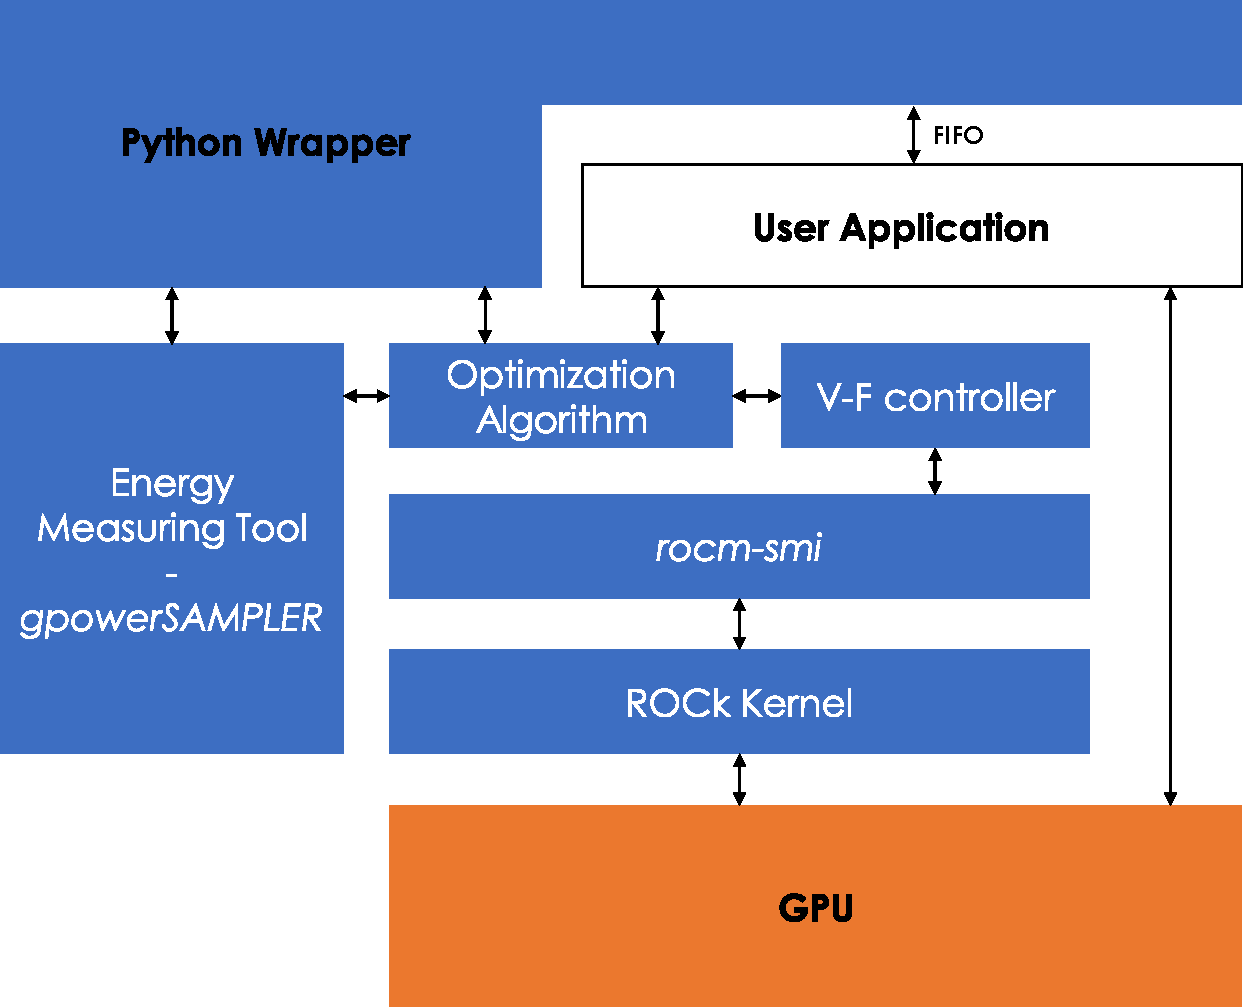
\includegraphics[width=0.6\textwidth]{Figures/Optimization/layerDiagram.pdf}
  \caption{Layer diagram of the developed V-F Optimization Mechanism. The blocks colored in blue represent the developed parts of the optimization mechanism developed in the context of this dissertation.}
  \label{fig:layer}
\end{figure}


\section{Library description}
\label{sec:usage}

This section describes how users should include the V-F optimization mechanism on their \acrshort{gpgpu} applications. As indicated, the wrapper that provides all the functions to enable this mechanism was developed in Python. However, the description of the functions provided ahead should allow for porting the same for others programming languages.

\textbf{def initOptimizationMechanism(pathToCharacterizationResults):}

Analyzes the user-provided Usable Execution Space file and queries the device \acrshort{dvfs} control interface (rocm-smi on the current implementation) to guarantee that the indicated frequency and voltage ranges are allowed by the target device.

\textbf{def initMesurements():}

Initiates the execution time and energy consumption measurement (gpowerSAMPLER on the current implementation).

\textbf{def computeMesurements(baseline=None):}

Indicates to end of the execution time and energy consumption measurement (gpowerSAMPLER on the current implementation) and returns both results. If the argument baseline, containing the baseline performance and energy measurement values, is provided, the output is normalized to each baseline value.


\textbf{def analiseOutput(output):}

A method that should be implemented by the developer that analyzes the user application output to determine its validity. The function returns a boolean indicating the ser application output validity.
    
\textbf{def optimizationMechanismSpaceExploration(measurements, optimizationMetric="EDP", outputValid=None):}

Analyzes application measurements and apply the new V-F configuration. The function receives the performance and energy measurements, the optimization metric and the results of the application output validity and implements the Simulated Annealing algorithm to accept or reject the tested V-F pair in accordance with the current \textit{V-F pair baseline}. If the configuration is accepted, the current \textit{V-F pair baseline} becomes the tested V-F pair. The method returns if the tested pair was accepted or not. It also implements the Online Monitorization phase.


\textbf{def optimizationMechanismFineTunning(measurements, optimizationMetric="EDP", outputValid=None):}

Similar to the previous function, however it implements the Hill-Climbing algorithm as Probabilistic Technique.


Listing~\ref{lst:wrapper} provides an example of the order and place where each function call should be performed and where the user should insert its application code.


\begin{lstlisting}[language=Python, caption=Usage example of the V-F Optimization Mechanism Library. Blue statements represents the added programming elements for the mechanism, label=lst:wrapper, basicstyle=\footnotesize\ttfamily,abovecaptionskip=0pt, captionpos=b,escapechar=@]
    @\textcolor{blue}{\textbf{initOptimizationMechanism(pathToCharacterizationResults)}}@
    ... initiate user application ...
    @\textcolor{blue}{\textbf{initMesurements()}}@
    ... execute baseline execution ...
    baselineMeasurements = @\textcolor{blue}{\textbf{computeMesurements()}}@
    @\textcolor{blue}{\textbf{rejected = 0}}@
    @\textcolor{blue}{\textbf{executedIterations = 0}}@
    for epoch in range(space_exploration_epochs):
        @\textcolor{blue}{\textbf{initMesurements()}}@
        ... code of application step ...
        measurements = @\textcolor{blue}{\textbf{computeMesurements(baselineMeasurements)}}@
        ... other necessary user application iteration operations that do not account
        for the user algorithm execution ...
        outputValid = @\textcolor{blue}{\textbf{analiseOutput(output)}}@
        
        # analyses the measurements, application output, temperature
        # generates and applies new V-F configuration
        @\textcolor{blue}{\textbf{accepted = optimizationMechanismSpaceExploration(measurements, outputValid)}}@
        @\textcolor{blue}{\textbf{executedIterations += 1}}@
        @\textcolor{blue}{\textbf{if accepted == False:}}@
            @\textcolor{blue}{\textbf{rejected += 1}}@
        @\textcolor{blue}{\textbf{if rejected == 5:}}@
            @\textcolor{blue}{\textbf{break}}@
    
    for epoch in range(total_number_of_epochs - executedIterations):
        @\textcolor{blue}{\textbf{initMesurements()}}@
        ... code of application step ...
        @\textcolor{blue}{\textbf{measurements = computeMesurements(baselineMeasurements)}}@
         ... other necessary user application iteration operations that do not account
        for the user algorithm execution ...
        outputValid = @\textcolor{blue}{\textbf{analiseOutput(output)}}@
        
        # analyses the measurements, application output, temperature
        # generates and applies new V-F configuration
        @\textcolor{blue}{\textbf{optimizationMechanismFineTunning(measurements, outputValid)}}@
\end{lstlisting}





\section{Summary}

The development of the V-F Optimization Mechanism that was described in this chapter fulfills the objective of having a concrete application to enable a non-conventional \acrshort{dvfs} system. The devised mechanism uses the previous chapter's experimental results to provide the user with convenient models that support the uncover V-F pairs to extract better energy-efficiency of their devices, without having any detailed knowledge of the \acrshort{gpu} architecture.

The following chapter demonstrates and evaluates the application of both the characterization and optimization mechanisms to improve the energy-efficiency of the Vega 10 \acrshort{gpu} when running deep learning applications.

 % file "Thesis_Opt_Mech.tex"
\cleardoublepage

%%%%%%%%%%%%%%%%%%%%%%%%%%%%%%%%%%%%%%%%%%%%%%%%%%%%%%%%%%%%%%%%%%%%%%%%
%                                                                      %
%     File: Thesis_Results.tex                                         %
%     Tex Master: Thesis.tex                                           %
%                                                                      %
%     Author: Andre C. Marta                                           %
%     Last modified :  2 Jul 2015                                      %
%                                                                      %
%%%%%%%%%%%%%%%%%%%%%%%%%%%%%%%%%%%%%%%%%%%%%%%%%%%%%%%%%%%%%%%%%%%%%%%%

\chapter{Application to Deep Learning}
\label{chapter:results}

Insert your chapter material here...


%%%%%%%%%%%%%%%%%%%%%%%%%%%%%%%%%%%%%%%%%%%%%%%%%%%%%%%%%%%%%%%%%%%%%%%%
\section{Deep Learning Overview}
\label{section:problem}

\subsection{Deep Neural Networks}
\subsubsection{Convolution Layers}
\subsubsection{Fully-Connected Layers}
\subsubsection{Reduction Layers}
\subsubsection{Recurrent Layers}

\subsection{Training and Inference}

\subsection{High-Level Libraries}

%%%%%%%%%%%%%%%%%%%%%%%%%%%%%%%%%%%%%%%%%%%%%%%%%%%%%%%%%%%%%%%%%%%%%%%%
\section{Experimental Methodology and Setup}
\label{section:methodology}

%%%%%%%%%%%%%%%%%%%%%%%%%%%%%%%%%%%%%%%%%%%%%%%%%%%%%%%%%%%%%%%%%%%%%%%%
\section{Non-conventional V-F on CNNs}
\label{section:baseline}

\subsection{CNN Layer Characterization with independent V-F scaling}

\subsubsection{Convolution Layers}
\subsubsection{Fully-Connected Layers}
\subsubsection{Reduction Layers}

\subsection{Error Analysis}
%%%%%%%%%%%%%%%%%%%%%%%%%%%%%%%%%%%%%%%%%%%%%%%%%%%%%%%%%%%%%%%%%%%%%%%%
\section{Complete CNNs training with non-conventional V-F}
\label{section:enhanced}

\subsection{Feasibility Assessment}
Vou mostrar que treinar com estas settings nao estraga accuracy

\subsection{Performance and energy optimization}

\section{Summary}
% % ----------------------------------------------------------------------
% \subsection{Figures}
% \label{subsection:figures}

% Insert your section material and possibly a few figures...

% Make sure all figures presented are referenced in the text!


% % ----------------------------------------------------------------------
% \subsubsection{Images}
% \label{subsection:images}

% \begin{figure}[!htb]
%   \centering
%   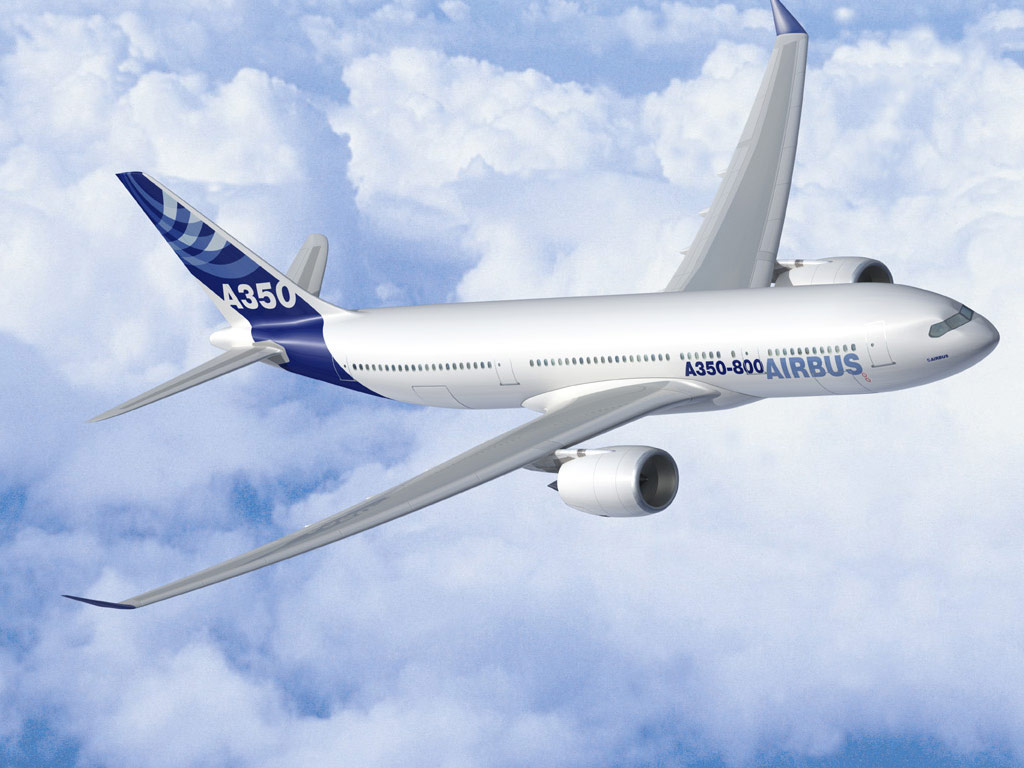
\includegraphics[width=0.25\textwidth]{Figures/Airbus_A350.jpg}
%   \caption[Caption for figure in TOC.]{Caption for figure.}
%   \label{fig:airbus1}
% \end{figure}

% \begin{figure}[!htb]
%   \begin{subfigmatrix}{2}
%     \subfigure[Airbus A320]{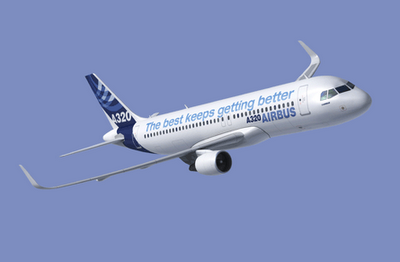
\includegraphics[width=0.49\linewidth]{Figures/Airbus_A320_sharklets.png}}
%     \subfigure[Bombardier CRJ200]{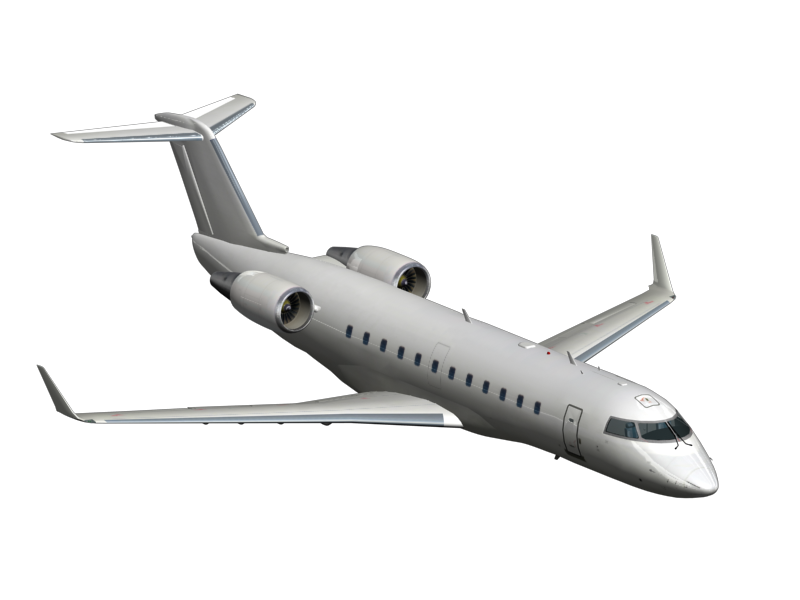
\includegraphics[width=0.49\linewidth]{Figures/Bombardier_CRJ200.png}}
%   \end{subfigmatrix}
%   \caption{Some aircrafts.}
%   \label{fig:aircrafts}
% \end{figure}

% Make reference to Figures \ref{fig:airbus1} and \ref{fig:aircrafts}.

% By default, the supported file types are {\it .png,.pdf,.jpg,.mps,.jpeg,.PNG,.PDF,.JPG,.JPEG}.

% See \url{http://mactex-wiki.tug.org/wiki/index.php/Graphics_inclusion} for adding support to other extensions.


% % ----------------------------------------------------------------------
% \subsubsection{Drawings}
% \label{subsection:drawings}

% Insert your subsection material and for instance a few drawings...

% The schematic illustrated in Fig.~\ref{fig:algorithm} can represent some sort of algorithm.

% \begin{figure}[!htb]
%   \centering
%   \scriptsize
% %  \footnotesize 
% %  \small
%   \setlength{\unitlength}{0.9cm}
%   \begin{picture}(8.5,6)
%     \linethickness{0.3mm}

%     \put(3,6){\vector(0,-1){1}}
%     \put(3.5,5.4){$\bf \alpha$}
%     \put(3,4.5){\oval(6,1){}}
%     %\put(0,4){\framebox(6,1){}}
%     \put(0.3,4.4){Grid Generation: \quad ${\bf x} = {\bf x}\left({\bf \alpha}\right)$}

%     \put(3,4){\vector(0,-1){1}}
%     \put(3.5,3.4){$\bf x$}
%     \put(3,2.5){\oval(6,1){}}
%     %\put(0,2){\framebox(6,1){}}
%     \put(0.3,2.4){Flow Solver: \quad ${\cal R}\left({\bf x},{\bf q}\left({\bf x}\right)\right) = 0$}

%     \put(6.0,2.5){\vector(1,0){1}}
%     \put(6.4,3){$Y_1$}

%     \put(3,2){\vector(0,-1){1}}
%     \put(3.5,1.4){$\bf q$}
%     \put(3,0.5){\oval(6,1){}}
%     %\put(0,0){\framebox(6,1){}}
%     \put(0.3,0.4){Structural Solver: \quad ${\cal M}\left({\bf x},{\bf q}\left({\bf x}\right)\right) = 0$}

%     \put(6.0,0.5){\vector(1,0){1}}
%     \put(6.4,1){$Y_2$}

%     %\put(7.8,2.5){\oval(1.6,5){}}
%     \put(7.0,0){\framebox(1.6,5){}}
%     \put(7.1,2.5){Optimizer}
%     \put(7.8,5){\line(0,1){1}}
%     \put(7.8,6){\line(-1,0){4.8}}
%   \end{picture}
%   \caption{Schematic of some algorithm.}
%   \label{fig:algorithm}
% \end{figure}


% % ----------------------------------------------------------------------
% \subsection{Equations}
% \label{subsection:equations}

% Equations can be inserted in different ways.

% The simplest way is in a separate line like this

% \begin{equation}
%   \frac{{\rm d} q_{ijk}}{{\rm d} t} + {\cal R}_{ijk}({\bf q}) = 0 \,.
% \label{eq:ode}
% \end{equation}

% If the equation is to be embedded in the text. One can do it like this ${\partial {\cal R}}/{\partial {\bf q}}=0$.

% It may also be split in different lines like this

% \begin{eqnarray}
%   {\rm Minimize}   && Y({\bf \alpha},{\bf q}({\bf \alpha}))            \nonumber           \\
%   {\rm w.r.t.}     && {\bf \alpha} \,,                                 \label{eq:minimize} \\
%   {\rm subject~to} && {\cal R}({\bf \alpha},{\bf q}({\bf \alpha})) = 0 \nonumber           \\
%                   &&       C ({\bf \alpha},{\bf q}({\bf \alpha})) = 0 \,. \nonumber
% \end{eqnarray}

% It is also possible to use subequations. Equations~\ref{eq:continuity}, \ref{eq:momentum} and \ref{eq:energy} form the Naver--Stokes equations~\ref{eq:NavierStokes}.

% \begin{subequations}
%     \begin{equation}
%     \frac{\partial \rho}{\partial t} + \frac{\partial}{\partial x_j}\left( \rho u_j \right) = 0 \,,
%     \label{eq:continuity}
%     \end{equation}
%     \begin{equation}
%     \frac{\partial}{\partial t}\left( \rho u_i \right) + \frac{\partial}{\partial x_j} \left( \rho u_i u_j + p \delta_{ij} - \tau_{ji} \right) = 0, \quad i=1,2,3 \,,
%     \label{eq:momentum}
%     \end{equation}
%     \begin{equation}
%         \frac{\partial}{\partial t}\left( \rho E \right) + \frac{\partial}{\partial x_j} \left( \rho E u_j + p u_j - u_i \tau_{ij} + q_j \right) = 0 \,.
%     \label{eq:energy}
%     \end{equation}
% \label{eq:NavierStokes}%
% \end{subequations}


% % ----------------------------------------------------------------------
% \subsection{Tables}
% \label{section:tables}

% Insert your subsection material and for instance a few tables...

% Make sure all tables presented are referenced in the text!

% Follow some guidelines when making tables:

% \begin{itemize}
%   \item Avoid vertical lines
%   \item Avoid “boxing up” cells, usually 3 horizontal lines are enough: above, below, and after heading
%   \item Avoid double horizontal lines
%   \item Add enough space between rows
% \end{itemize}

% \begin{table}[!htb]
%   \renewcommand{\arraystretch}{1.2} % more space between rows
%   \centering
%   \begin{tabular}{lccc}
%     \toprule
%     Model           & $C_L$ & $C_D$ & $C_{M y}$ \\
%     \midrule
%     Euler           & 0.083 & 0.021 & -0.110    \\
%     Navier--Stokes  & 0.078 & 0.023 & -0.101    \\
%     \bottomrule
%   \end{tabular}
%   \caption[Table caption shown in TOC.]{Table caption.}
%   \label{tab:aeroCoeff}
% \end{table}

% Make reference to Table \ref{tab:aeroCoeff}.

% Tables \ref{tab:memory} and \ref{tab:multipleColumns} are examples of tables with merging columns:

% \begin{table}[!htb]
%   \renewcommand{\arraystretch}{1.2} % more space between rows
%   \centering
%   \begin{tabular}[]{lrr}
%     \toprule
%                 & \multicolumn{2}{c}{\underline{Virtual memory [MB]}} \\
%                 & Euler       & Navier--Stokes \\
%     \midrule
%       Wing only &  1,000      &    2,000       \\
%       Aircraft  &  5,000      &   10,000       \\
%       (ratio)   & $5.0\times$ & $5.0\times$    \\
%     \bottomrule
%   \end{tabular}
%   \caption{Memory usage comparison (in MB).}
%   \label{tab:memory}
% \end{table}

% \begin{table}[!htb]
%   \centering
%   \renewcommand{\arraystretch}{1.2} % more space between rows
%   \begin{tabular}{@{}rrrrcrrr@{}} % remove space to the vertical edges @{}...@{}
%     \toprule
%       & \multicolumn{3}{c}{$w = 2$} & \phantom{abc} & \multicolumn{3}{c}{$w = 4$} \\
%     \cmidrule{2-4}
%     \cmidrule{6-8}
%       & $t=0$ & $t=1$ & $t=2$ && $t=0$ & $t=1$ & $t=2$ \\
%     \midrule
%       $dir=1$
%       \\
%       $c$ &  0.07 &  0.16 &  0.29 &&  0.36 &  0.71 &   3.18 \\
%       $c$ & -0.86 & 50.04 &  5.93 && -9.07 & 29.09 &  46.21 \\
%       $c$ & 14.27 &-50.96 &-14.27 && 12.22 &-63.54 &-381.09 \\
%       $dir=0$
%       \\
%       $c$ &  0.03 &  1.24 &  0.21 &&  0.35 & -0.27 &  2.14 \\
%       $c$ &-17.90 &-37.11 &  8.85 &&-30.73 & -9.59 & -3.00 \\
%       $c$ &105.55 & 23.11 &-94.73 &&100.24 & 41.27 &-25.73 \\
%     \bottomrule
%   \end{tabular}
%   \caption{Another table caption.}
%   \label{tab:multipleColumns}
% \end{table}

% An example with merging rows can be seen in Tab.\ref{tab:multipleRows}.

% \begin{table}[!htb]
%   \renewcommand{\arraystretch}{1.2} % more space between rows
%   \centering
%   \begin{tabular}{ccccc}
%     \toprule
%       \multirow{2}{*}{ABC} & \multicolumn{4}{c}{header} \\
%       \cmidrule{2-5} & 1.1 & 2.2 & 3.3 & 4.4 \\
%     \midrule
%       \multirow{2}{*}{IJK} & \multicolumn{2}{c}{\multirow{2}{*}{group}} & 0.5 & 0.6 \\
%       \cmidrule{4-5}       & \multicolumn{2}{c}{}                       & 0.7 & 1.2 \\
%     \bottomrule
%   \end{tabular}
%   \caption{Yet another table caption.}
%   \label{tab:multipleRows}
% \end{table}

% If the table has too many columns, it can be scaled to fit the text widht, as in Tab.\ref{tab:scale}.
% \begin{table}[!htb]
%   \renewcommand{\arraystretch}{1.2} % more space between rows
%   \centering
%   \resizebox*{\textwidth}{!}{%
%     \begin{tabular}[]{lcccccccccc}
%       \toprule
%         Variable &  a  &  b  &  c  &  d  &  e  &  f  &  g  &  h  &  i  &  j  \\
%       \midrule
%         Test 1   &  10,000 &  20,000 &  30,000 &  40,000 &  50,000 &  60,000 &  70,000 &  80,000 &  90,000 & 100,000 \\
%         Test 2   &  20,000 &  40,000 &  60,000 &  80,000 & 100,000 & 120,000 & 140,000 & 160,000 & 180,000 & 200,000 \\
%       \bottomrule
%     \end{tabular}
%   }%
%   \caption{Very wide table.}
%   \label{tab:scale}%
% \end{table}


% % ----------------------------------------------------------------------
% \subsection{Mixing}
% \label{section:mixing}

% If necessary, a figure and a table can be put side-by-side as in Fig.\ref{fig:side_by_side}

% \begin{figure}[!htb]
%   \begin{minipage}[b]{0.60\linewidth}
%     \centering
%     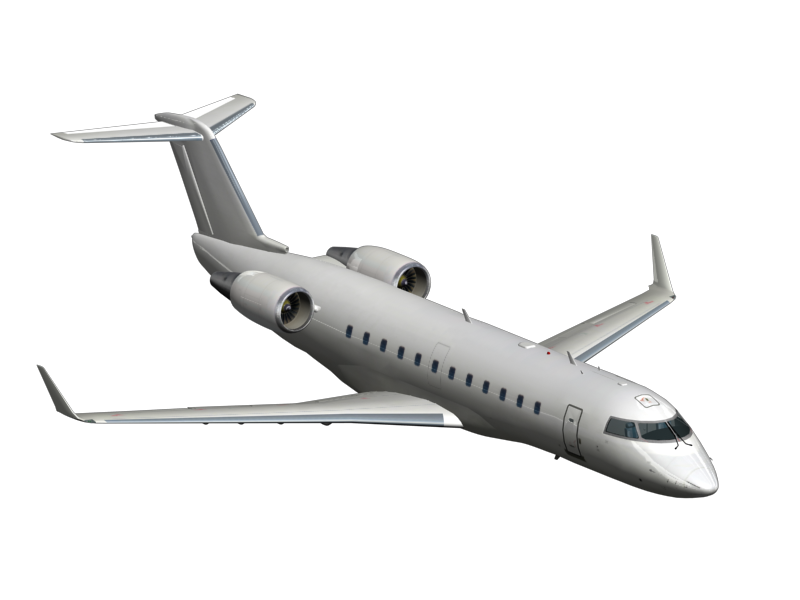
\includegraphics[width=\linewidth]{Figures/Bombardier_CRJ200}
%   \end{minipage}%
%   \begin{minipage}[b]{0.30\linewidth}
%     \centering
%     \begin{tabular}[b]{lll}
%       \toprule
%         \multicolumn{3}{c}{Legend} \\
%       \midrule
%         A & B & C \\
%         0 & 0 & 0 \\
%         0 & 1 & 0 \\
%         1 & 0 & 0 \\
%         1 & 1 & 1 \\
%       \bottomrule
%     \end{tabular}
%     \vspace{5em}
%   \end{minipage}
% \caption{Figure and table side-by-side.}
% \label{fig:side_by_side}
% \end{figure}

 % file "Thesis_Results.tex"
\cleardoublepage

%\input{Thesis_new_file} % add new .tex files for new chapters
% \cleardoublepage

%\input{Thesis_new_file} % add new .tex files for new chapters
% \cleardoublepage



%%%%%%%%%%%%%%%%%%%%%%%%%%%%%%%%%%%%%%%%%%%%%%%%%%%%%%%%%%%%%%%%%%%%%%%%
%                                                                      %
%     File: Thesis_Conclusions.tex                                     %
%     Tex Master: Thesis.tex                                           %
%                                                                      %
%     Author: Andre C. Marta                                           %
%     Last modified :  2 Jul 2015                                      %
%                                                                      %
%%%%%%%%%%%%%%%%%%%%%%%%%%%%%%%%%%%%%%%%%%%%%%%%%%%%%%%%%%%%%%%%%%%%%%%%

\chapter{Conclusions}
\label{chapter:conclusions}

Insert your chapter material here...



% ----------------------------------------------------------------------
\section{Future Work}
\label{section:future}

A few ideas for future work...

 % file "Thesis_Conclusions.tex"
\cleardoublepage

% ----------------------------------------------------------------------
%  Bibliography
% ----------------------------------------------------------------------

% Add entry in the table of contents as chapter
\phantomsection
\addcontentsline{toc}{chapter}{\bibname}

% Include all references in .bib file, even non-cited ones...
%\nocite{*} % this should be used carefully because it is not correct!

% Produces the bibliography section when processed by BibTeX
%
% Bibliography style
% > entries ordered alphabetically
%\bibliographystyle{plain}
% > unsorted with entries appearing in the order in which the citations appear.
%\bibliographystyle{unsrt}
% > entries ordered alphabetically, with first names and names of journals and months abbreviated
%\bibliographystyle{abbrv}
% > entries ordered alphabetically, with reference markers based on authors' initials and publication year
%\bibliographystyle{alpha}
%
% Replacement bibliography styles provided by 'natbib' package
% (plainnat.bst, abbrvnat.bst, unsrtnat.bst )
% > entries ordered alphabetically
%\bibliographystyle{plainnat}
% > unsorted with entries appearing in the order in which the citations appear.
%\bibliographystyle{unsrtnat}
% > entries ordered alphabetically, with first names and names of journals and months abbreviated
%\bibliographystyle{abbrvnat} % <<<<< SELECT IF USING REFERENCES BY AUTHOR/YEAR
% > entries ordered alphabetically, with reference markers based on authors' initials and publication year
%\bibliographystyle{alpha}
%
% Custom bibliography style adapted from 'natbib' package
%   (based on http://tex.stackexchange.com/questions/5053/is-it-possible-to-get-unsrt-abbrv-bibliography)
%   (unsrtnat.bst + abbrvnat.bst -> abbrvunsrtnat.bst)
%   (original files copied from:
%   http://tug.ctan.org/macros/latex/contrib/natbib/abbrvnat.bst
%   http://tug.ctan.org/macros/latex/contrib/natbib/unsrtnat.bst
% > unsorted with entries appearing in the order in which the citations appear, with first names and names of journals and months abbreviated.
\bibliographystyle{abbrvunsrtnat} % <<<<< SELECT IF USING REFERENCES BY NUMBER (CITATION ORDER)

% External bibliography database file in the BibTeX format
% \bibliography{Thesis_bib_DB} % file "Thesis_bib_DB.bib"
\bibliography{references} % file "Thesis_bib_DB.bib"

\cleardoublepage

% ----------------------------------------------------------------------
%  Appendix (optional)
%
%  CAUTION: 1) the main document (up to the conclusions) shall not exceed 80 pages
%           2) the document shall not exceed a total of 100 pages (per IST regulations)
% ----------------------------------------------------------------------
\appendix

% add page number prefix according to apendix chapter (optional)
%\renewcommand{\thepage}{\thechapter.\arabic{page}}

% re-set arabic numbering (A.1,A.2,...) (optional, use only if chapter prefix is added)
%\setcounter{page}{1}

%%%%%%%%%%%%%%%%%%%%%%%%%%%%%%%%%%%%%%%%%%%%%%%%%%%%%%%%%%%%%%%%%%%%%%%%
%                                                                      %
%     File: Thesis_Appendix_A.tex                                      %
%     Tex Master: Thesis.tex                                           %
%                                                                      %
%     Author: Andre C. Marta                                           %
%     Last modified :  2 Jul 2015                                      %
%                                                                      %
%%%%%%%%%%%%%%%%%%%%%%%%%%%%%%%%%%%%%%%%%%%%%%%%%%%%%%%%%%%%%%%%%%%%%%%%

\chapter{How to independently control and set the desired V-F pair}
\label{chapter:appendixRocm-smi}

As introduced in this dissertation, the independent control of frequency and voltage is not widely available, and only recently, AMD allows it through their ROCm software stack, more specifically through rocm-smi - ROCm system management interface. However, even the most recent version of this tool (presented on ROCm 3.8) does not provide an easy and utterly understandable way of setting the desired frequency and voltage pair. This Annex intends to describe how to command the rocm-smi tool to control and set the desired V-F pair in the two tested GPUs, AMD Vega 10 Frontier Edition and AMD Radeon 5700 XT.

As described in Chapter 2, rocm-smi is a Linux command line application. When launch, it prompts the interface exhibited in Figure~\ref{fig:rocm-smi} where it is possible to check the device temperature, average device power, core domain clock - \texttt{sclk}, \acrshort{dvfs} domain clock - \texttt{mclk}, percentage of fan speed, \texttt{perf} - indicating current DVFS setting as automatic or manual, current device power cap and finally, DRAM and Core utilization.

\begin{figure}[htb]
    \centering
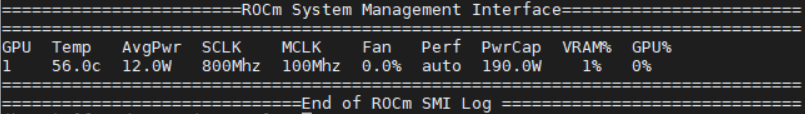
\includegraphics[width=0.75\textwidth]{Figures/AnnexA/rocm-smi.png}
        \caption{Rocm-smi interface.}
    \label{fig:rocm-smi}
\end{figure}


The V-F settings' control depends on the current device underuse due to different implementations of their \acrshort{dvfs} system. However, \texttt{perf} configuration and device power cap have to be changed regardless of the implementation of the \acrshort{dvfs} system. 

The following enumeration describes the steps to be made regardless of the implementation of the \acrshort{dvfs} system, stressing the reasons for the same. The following sections detail the working and tunning of the V-F pair for each of the tested \acrshort{gpu}s.

\begin{enumerate}
\item \textbf{Change device performance level:} Disable automatic \acrshort{dvfs} system.\\
\texttt{rocm-smi --setperflevel manual}
\item \textbf{Get device maximum power cap:} Get maximum allowed power consumption (PowerCap) allowed by the device. \\
\texttt{rocm-smi --showmaxpower} 
\item \textbf{Change device power cap:} Change the current device maximum power consumption to the value obtained on the previvous command.\\
\texttt{rocm-smi --setpoweroverdrive X --autorespond yes}
\end{enumerate}

It is necessary to change the default PowerCap value to fully unlock manual tunning of the \acrshort{dvfs} system. If not changed, the device will not allow sustained configuration of the highest frequency and voltage levels.

\section{AMD Vega 10 Frontier Edition}

The Vega 10 \acrshort{gpu} presents the concept of discrete performance levels, containing eight possible configurations for the core \acrshort{dvfs} domain. 
When editing the frequency and voltage values of each performance level, three rules must be followed. If that is not the case, even though the system accepts the configuration, the \texttt{perf} configuration (performance level) switches to automatic. The rules are 

\begin{enumerate}
\item the desired frequency and voltage values must be within the valid ranges for the target device; 
\item the desired frequency and voltage values cannot have the same value as the default for the given performance level; 
\item the selected frequency and voltage values of the performance level $i$ need to be at least 1 unit (1 MHz or 1 mV) above the performance level $i-1$ and one unit below the performance level $i+1$.
\end{enumerate}

To guarantee that the desired V-F pair is selected, it is necessary to write on performance level 0 to 6 V-F pairs below all configurations that will be used and apply on the performance level 7 the desired V-F pair. In this way, even some automatic control systems that may remain active are forced to select the wanted configuration. Table~\ref{tab:gpulevels-tunning} presents the pre-defined voltage values for the performance levels.

\begin{table}[!htb]
\centering
\begin{tabular}{ccc}
\textbf{Level} & \textbf{Frequency {[}MHz{]}} & \textbf{Voltage {[}mV{]}}  \\ \hline
0              & 853                          & 801                        \\
1              & 860                          & 810                      \\
2              & 870                          & 820                       \\
3              & 880                          & 830                      \\ 
4              & 890                          & 840                      \\
5              & 900                          & 850                     \\
6              & 910                          & 860                       \\
7              & \texttt{Desired Frequency}   & \texttt{Desired Voltage}                     \\ \hline
\end{tabular}
\caption{Vega 10 GPU core performance levels general configuration.}
\label{tab:gpulevels-tunning}
\end{table}

The following enumeration indicates the rocm-smi commands that should be executed to select the desired voltage-frequency configuration.

\begin{enumerate}
\setcounter{enumi}{3}
\item \textbf{Change performance levels 0 to 6 to pre defined values:} \\
\texttt{rocm-smi --setslevel 0 853 801 --autorespond yes}\\
\texttt{rocm-smi --setslevel 1 860 810 --autorespond yes}\\
\texttt{rocm-smi --setslevel 2 870 820 --autorespond yes}\\
\texttt{rocm-smi --setslevel 3 880 830 --autorespond yes}\\
\texttt{rocm-smi --setslevel 4 890 840 --autorespond yes}\\
\texttt{rocm-smi --setslevel 5 900 850 --autorespond yes}\\
\texttt{rocm-smi --setslevel 6 910 860 --autorespond yes}
\item \textbf{Change performance levels 7 to desired values:} \\
\texttt{rocm-smi --setslevel 7 \$frequency \$voltage --autorespond yes}
\item \textbf{Select core performance level 7:} \\
\texttt{rocm-smi --setsclk 7 --autorespond yes}
\item \textbf{Confirm the current voltage level:} To note that this command shows the voltage value that corresponds to $max(V_{Core}, V_{DRAM})$, so, if a voltage value is selected on the core domain is smaller than the current applied on the \acrshort{dram} domain, the tool will report the voltage value of the \acrshort{dram} domain.\\
\texttt{rocm-smi --showvoltage}
\end{enumerate}




\section{AMD Radeon 5700 XT}

The Radeon 5700 XT \acrshort{dvfs} system does not present the concept of performance levels. Instead, three V-F pairs indicated, and a quadratic regression is made to create the function $V(f)$ (chart presented in Chapter 2 Figure~\ref{fig:voltage_curve}). Similarly to the Vega 10 \acrshort{gpu}, the three V-F pairs also need to respect the three indicated rules.

\begin{figure}[htb]
    \centering
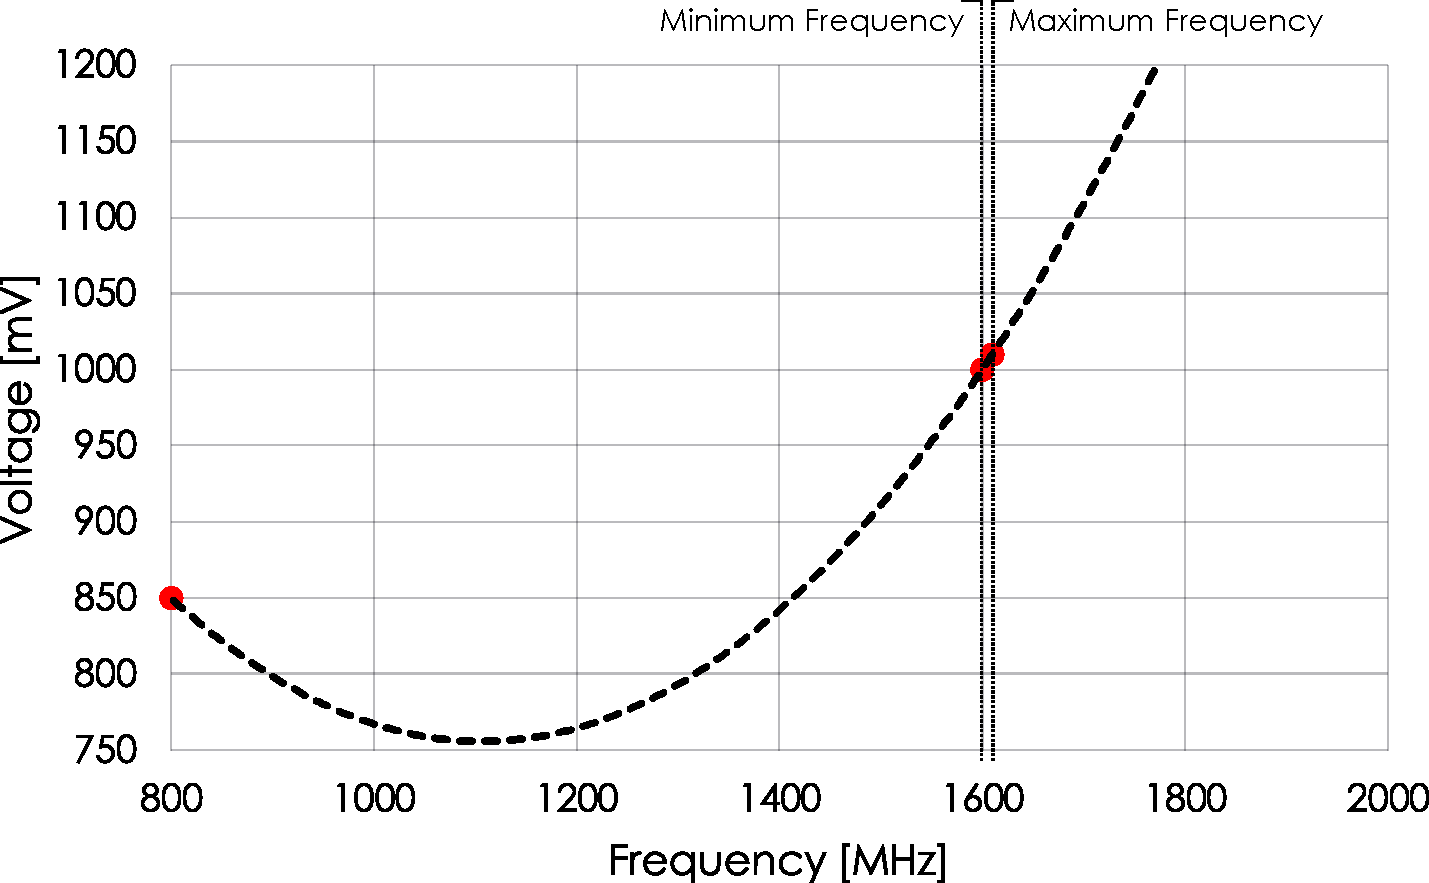
\includegraphics[width=0.75\textwidth]{Figures/AnnexA/vegadvfscontrol.pdf}
        \caption{Change in voltage curve to select a given V-F pair.}
    \label{fig:voltagecurvepair}
\end{figure}

Overall, to be able to select and apply a specific V-F pair, the rocm-smi interface presents one other command that indicates to the \acrshort{dvfs} system, which is the minimum and maximum frequency that should be used. Taking advantage of that interface, the devised method to select a given frequency is presented in Figure~\ref{fig:voltagecurvepair}, where the first V-F pair is not changed, and the remaining two are set following Table~\ref{tab:xt-pairs}. The value of $+10$ is the pre-defined allowed variation of the parameters and was decided taking into account the range of frequency and voltage values.



\begin{table}[!htb]
\centering
\begin{tabular}{ccc}
\textbf{V-F pair number} & \textbf{Frequency {[}MHz{]}} & \textbf{Voltage {[}mV{]}}  \\ \hline
0              & 800                          & 850                        \\
1              & \texttt{Desired Frequency}   & \texttt{Desired Voltage}                        \\
2              & \texttt{Desired Frequency} + 10   & \texttt{Desired Voltage} + 10                        \\\hline
\end{tabular}
\caption{Radeon 5700 XT GPU core V-F pairs general configuration.}
\label{tab:xt-pairs}
\end{table}


The following enumeration indicates the rocm-smi commands that should be executed to select the desired voltage-frequency configuration.

\begin{enumerate}
\setcounter{enumi}{3}
\item \textbf{Change the V-F pair values:} \\
\texttt{rocm-smi --setvc 0 800 850  --autorespond yes}\\
\texttt{rocm-smi --setvc 1 \$frequency \$voltage     --autorespond yes}\\
\texttt{rocm-smi --setvc 2 \$\{frequency + 10\} \$\{voltage + 10\}  --autorespond yes}
\item \textbf{Change allowed frequency range limits:} \\
\texttt{rocm-smi --setsrange 0 \$frequency --autorespond yes}\\
\texttt{rocm-smi --setsrange 1 \$\{frequency + 10\} --autorespond yes}
\item \textbf{Confirm the current voltage level:} To note that this command shows the voltage value that corresponds to $max(V_{Core}, V_{DRAM})$, so, if a voltage value is selected on the core domain is smaller than the current applied on the \acrshort{dram} domain, the tool will report the voltage value of the \acrshort{dram} domain.\\
\texttt{rocm-smi --showvoltage}
\end{enumerate}

 % file "Thesis_Appendix_A.tex"
\cleardoublepage

% re-set arabic numbering (B.1,B.2,...) (optional, use only if chapter prefix is added)
%\setcounter{page}{1}

% %%%%%%%%%%%%%%%%%%%%%%%%%%%%%%%%%%%%%%%%%%%%%%%%%%%%%%%%%%%%%%%%%%%%%%%%
%                                                                      %
%     File: Thesis_Appendix_B.tex                                      %
%     Tex Master: Thesis.tex                                           %
%                                                                      %
%     Author: Andre C. Marta                                           %
%     Last modified :  2 Jul 2015                                      %
%                                                                      %
%%%%%%%%%%%%%%%%%%%%%%%%%%%%%%%%%%%%%%%%%%%%%%%%%%%%%%%%%%%%%%%%%%%%%%%%

\chapter{Technical Datasheets}
\label{chapter:appendixDatasheets}

It is possible to add PDF files to the document, such as technical sheets of some equipment used in the work.

% ----------------------------------------------------------------------
\section{Some Datasheet}
\label{section:datasheet}

% See more options to include PDF files in
% http://mirror.unl.edu/ctan/macros/latex/contrib/pdfpages/pdfpages.pdf
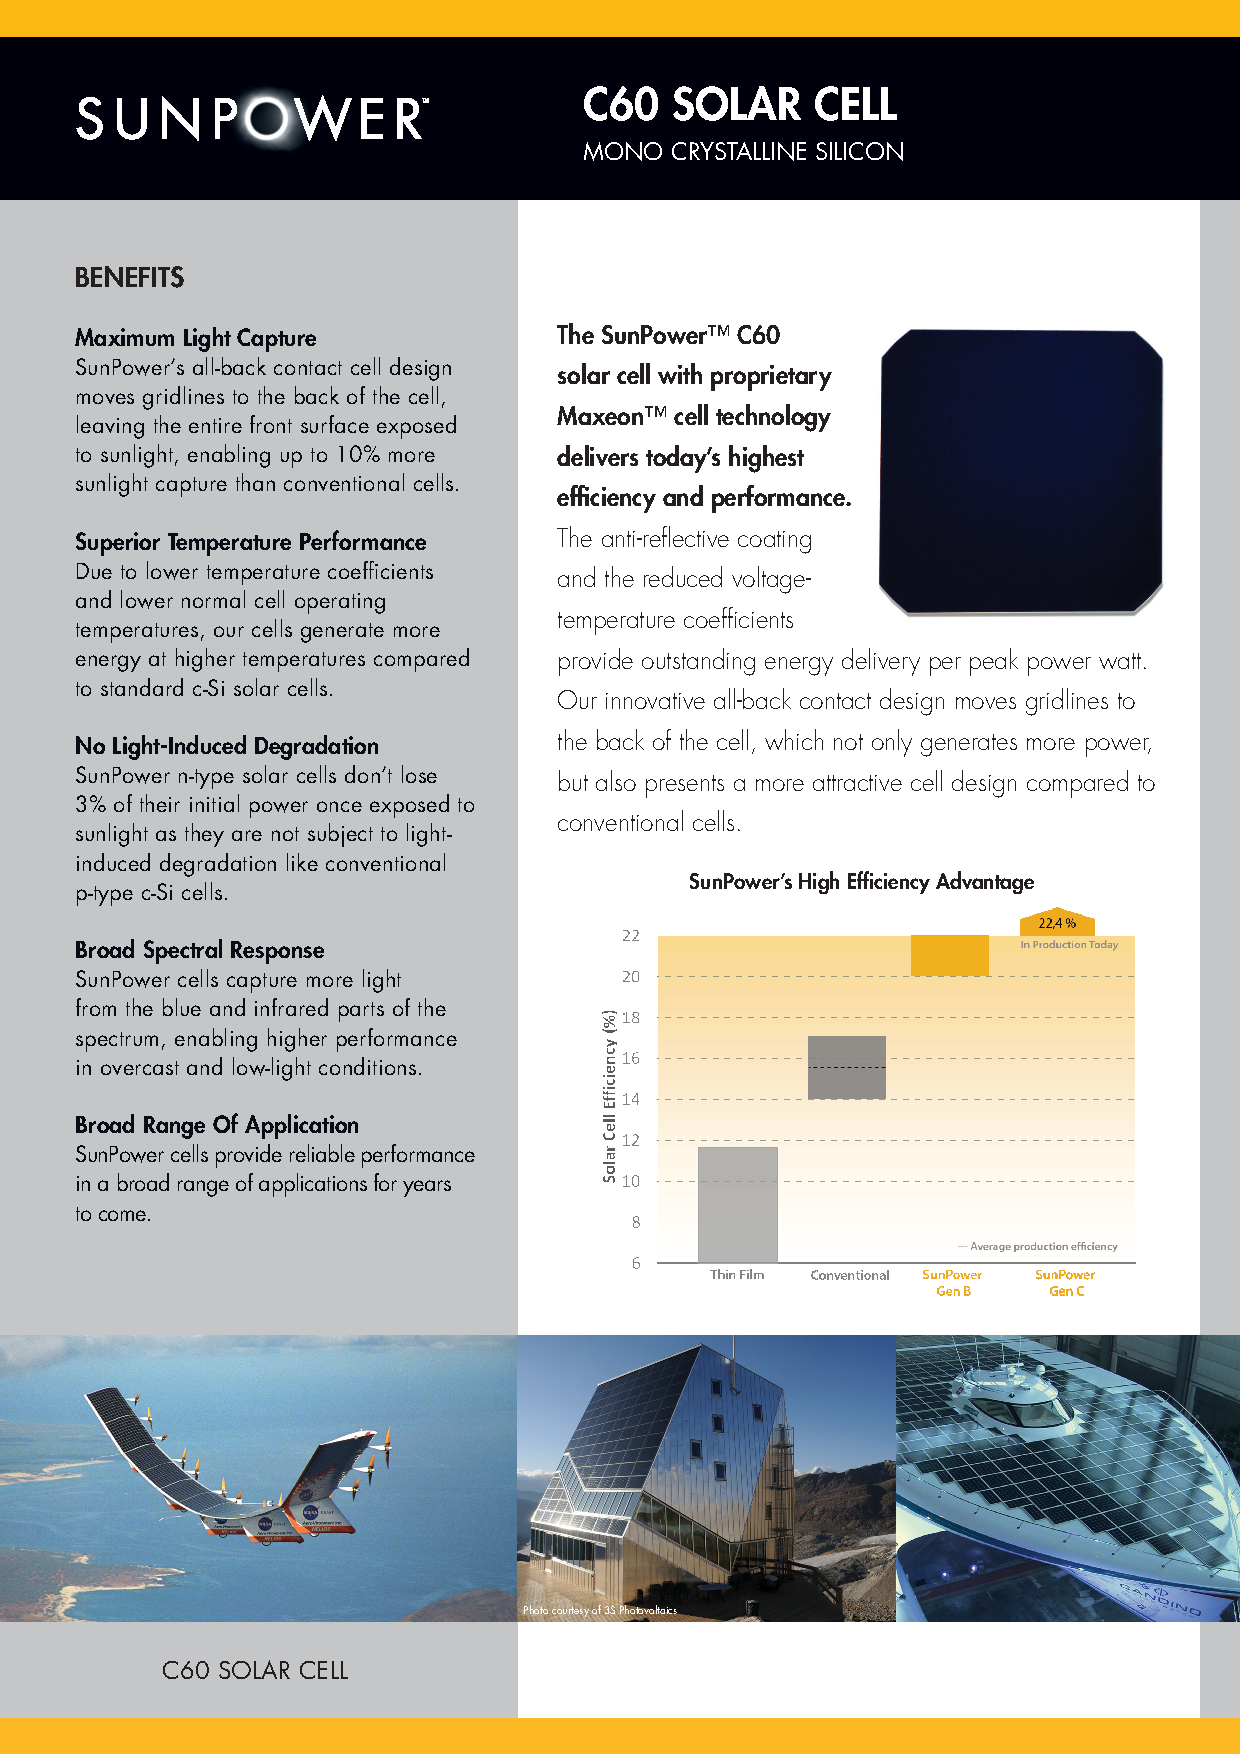
\includepdf[pages={1-2},nup=1x2,landscape=true]{Figures/SolarCell_Sunpower_C60.pdf}

 % file "Thesis_Appendix_B.tex"
% \cleardoublepage

% ----------------------------------------------------------------------
\end{document}
% ----------------------------------------------------------------------

